\documentclass[12pt,a4paper]{article}
\newcommand{\version}{4.0}

\usepackage{pdfpages}
\usepackage{url,graphicx,tabularx,array,titleref,booktabs}
\usepackage[hmargin=.47in,vmargin=0.6in,nohead]{geometry}
\usepackage{color,verbatim,framed}
\usepackage{moreverb}
\usepackage{xr}
%\usepackage{upgreek}
\usepackage{fancyvrb}
%\usepackage{fancyhdr}
\usepackage{amsmath}
\usepackage{appendix}
\usepackage{color}
\usepackage{tabularx}
\usepackage{graphicx}
%\usepackage{fullpage}
\usepackage{enumerate}
\usepackage{bold-extra}
%\usepackage{fix-cm}
\definecolor{txt}{rgb}{0,0,1}
\definecolor{cmd}{rgb}{0,1,0}
\newcommand{\txt}[1]{{\color{txt}{\tt #1}}}
\newcommand{\cmd}[1]{{\color{cmd}{\tt #1}}}
\definecolor{warwickdark}{cmyk}{1.0,0.6,0.0,0.06}
\definecolor{warwickmid}{cmyk}{0.69,0.34,0.0,0.0}
\definecolor{warwicklight}{cmyk}{1.0,0.0,0.0,0.0}
\definecolor{warwickred}{cmyk}{0.0,1.0,0.65,0.15}
\newcommand{\HRule}{\rule[0.3cm]{\linewidth}{0.5mm}}
\newcommand{\emphtext}{\color{warwickdark} \fontfamily{phv}\selectfont\large\bf}
\newcommand{\inlinecode}[1]{{\color{warwickred} \bf\texttt{#1}}}
\newcommand{\sect}[1]{Section~\ref{sec:#1}}
\newcommand{\sectit}[1]{``{\bf\titleref{sec:#1}}'' (\sect{#1})}
\newcommand{\code}[1]{{\texttt{#1}}}
%\newcommand{\qtt}[1]{``{\code{#1}}''}
\newcommand{\inlineemph}[1]{{\color{warwicklight} \bf{#1}}}
\newcommand{\inlineemtt}
  {\color{warwicklight}\fontfamily{phv}\selectfont\ttfamily\bfseries}
\newcommand{\cemph}[1]{{\inlineemph{#1}}}
\newcommand{\EPOCH}{{\color{warwickdark}\fontfamily{phv}\selectfont{EPOCH}}}
% Caption before Label to fix strange problem with not putting in subsection
% numbers. DO NOT CHANGE.
\newcommand{\captionedimage}[3]
  {{\begin{figure}[hbt!]\centering\includegraphics{#1}\caption{#3}\label{#2}
    \end{figure}}}
\newcommand{\scaledcapimage}[4]
  {{\begin{figure}[hbt!]\centering\includegraphics[scale=#4]{#1}\caption{#3}
    \label{#2} \end{figure}}}

\newcommand{\tony}[1]{{\color{warwickred} \bf{TONY'S COMMENT:} \bf{#1}}\\}

\definecolor{shadecolor}{cmyk}{0.1,0.05,0.0,0.0}
\setlength{\FrameRule}{0.6mm}

\newenvironment{lboxverbatim}[1]{
\setlength{\FrameSep}{0pt}
%\topsep=0ex\relax
\def\FrameCommand{\fboxsep=0pt \colorbox{shadecolor}}
\MakeFramed{\FrameRestore}
\vspace{-13.5pt}
\fvset{label=#1}
\boxverb
}{
\endboxverb
\vspace{-13.5pt}
\endMakeFramed
}
\newenvironment{boxverbatim}{\lboxverbatim{none}}{\endlboxverbatim}

\newenvironment{lboxverbatim2}[1]{
\setlength{\FrameSep}{0pt}
\topsep=0ex\relax
\def\FrameCommand{\fboxsep=0pt \colorbox{shadecolor}}
\MakeFramed{\FrameRestore}
\vspace{-13.5pt}
\fvset{label=#1}
\boxverb
}{
\endboxverb
\vspace{-13.5pt}
\endMakeFramed
}

\newenvironment{nbboxverbatim}[1]{
\noindent\minipage{\textwidth}
\setlength{\FrameSep}{0pt}
%\topsep=0ex\relax
\def\FrameCommand{\fboxsep=0pt \colorbox{shadecolor}}
\MakeFramed{\FrameRestore}
\fvset{label=#1}
\boxverb
}{
\endboxverb
\vspace{-13.5pt}
\endMakeFramed
\endminipage
\vspace{5pt}
}

\DefineVerbatimEnvironment{boxverb}{Verbatim}
  {frame=single,framerule=0.5mm,rulecolor=\color{warwickmid},
   formatcom=\color{black}}

\DefineVerbatimEnvironment{codedef}{Verbatim}
  {formatcom=\color{warwickred},fontsize=\Large,commandchars=\\\{\}}
%\newcommand{\txt}[1]{{\color{blue}{\tt #1}}}
%\newcommand{\cmd}[1]{{\color{green}{\tt #1}}}
\newcommand{\qtt}[1]{``{\tt #1}"}
\newcommand{\qm}[1]{{\em ``#1"}}

\setlength{\emergencystretch}{3em}

\externaldocument{epoch_dev}

\begin{document}%
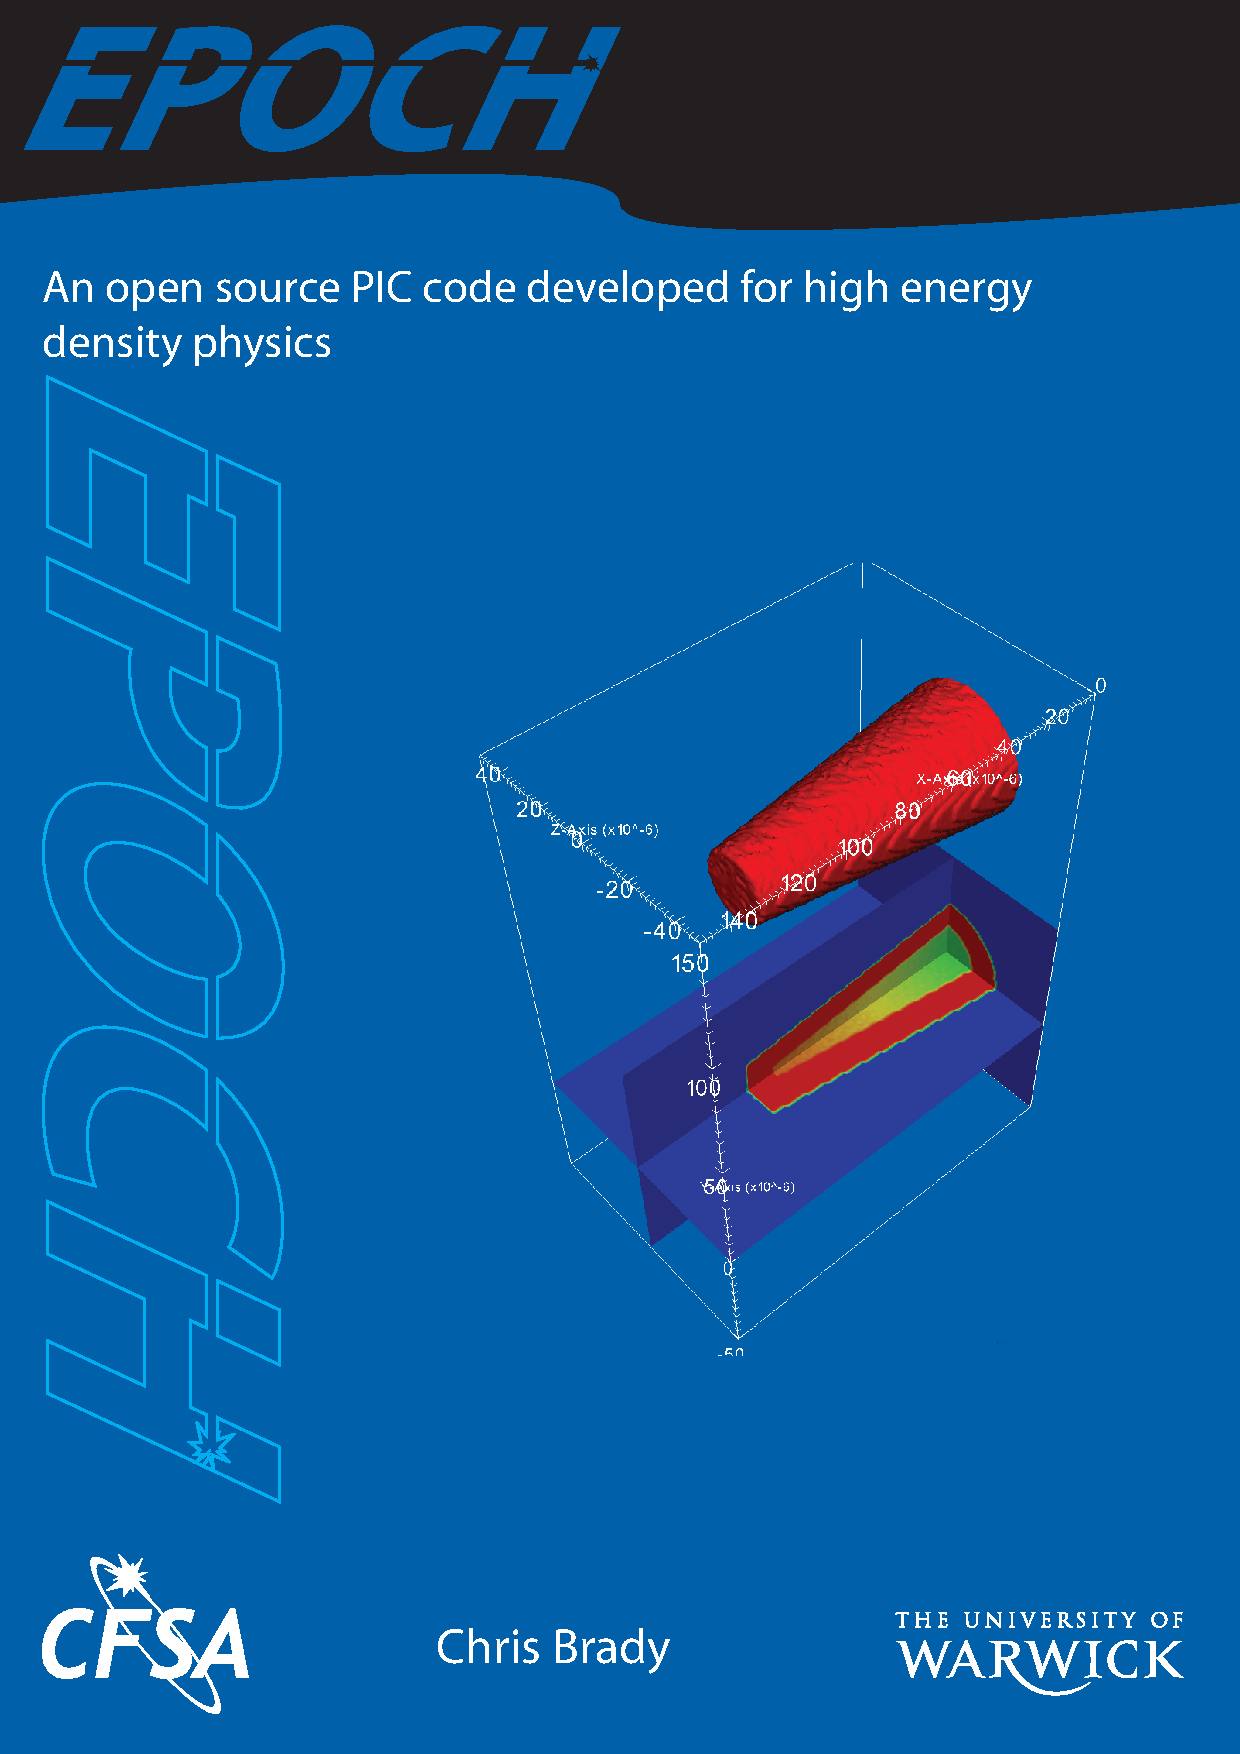
\includepdf{images/title_page_user}
{
  \fontfamily{phv}\selectfont\begin{titlepage}

\begin{center}

%This section borrows heavily from WikiBooks LaTeX

\includegraphics[width=14cm]{./images/EPOCHLogo}\\[1cm]

\textsc{\LARGE{University of Warwick}}\\[1.5cm]

% Title
\HRule\\[0.2cm]
{\huge\bfseries{Users Manual for the EPOCH PIC codes}}\\[0.4cm]
\HRule\\[1.5cm]

% Author and supervisor
\begin{minipage}{0.4\textwidth}
\begin{flushleft}\large%
\emph{Last revision by:}\\
Keith \textsc{Bennett}
\end{flushleft}
\end{minipage}
\begin{minipage}{0.4\textwidth}
\begin{flushright}\large%
\emph{EPOCH written by:} \\
Chris \textsc{Brady}\\
Keith \textsc{Bennett}\\
\end{flushright}
\end{minipage}

\vfill%
% Bottom of the page
{\large\today, {\EPOCH} Version \version}

\end{center}

\end{titlepage}

}
\fontfamily{garamond}\selectfont%
\tableofcontents%
\newpage%
\DefineShortVerb{\#}
\fvset{formatcom=\color{warwickred}}

\section{FAQs}

\subsection{Is this manual up to date?}

Whenever a new milestone version of {\EPOCH} is finalised, the version
number is changed and this manual is updated accordingly. The version number
of the manual should match the first two digits for that of the {\EPOCH}
source code.
This version number is printed to screen when you run the code. The line looks
something like the following:
\begin{boxverbatim}
 Welcome to EPOCH2D version 4.12.0   (commit v4.12.0-0-gfd74a464-clean)
\end{boxverbatim}
Here, only the number ``4.12'' is important.

Since version 3.1 of the manual, new additions and changes are mentioned
in the appendix.

\subsection{What is {\EPOCH}?}

{\EPOCH} is a plasma physics simulation code which uses the Particle in Cell
(PIC) method. In this method, collections of physical particles are represented
using a smaller number of pseudoparticles, and the fields generated by the
motion of these pseudoparticles are calculated using a finite difference time
domain technique on an underlying grid of fixed spatial resolution. The forces
on the pseudoparticles due to the calculated fields are then used to update the
pseudoparticle velocities, and these velocities are then used to update the
pseudoparticle positions. This leads to a scheme which can reproduce the full
range of classical micro-scale behaviour of a collection of charged
particles.

\subsubsection{Features of {\EPOCH}}
\begin{itemize}
  \item MPI parallelised, explicit, second-order, relativistic PIC code.
  \item Dynamic load balancing option for making optimal use of all processors
    when run in parallel.
  \item MPI-IO based output, allowing restart on an arbitrary number of
    processors.
  \item Data analysis and visualisation options include ITT IDL, LLNL VisIt,
    Mathworks MatLab and Matplotlib in Python.
  \item Control of setup and runs of {\EPOCH} through a customisable input deck.
\end{itemize}

\subsection{The origins of the code}
The {\EPOCH} family of PIC codes is based on the older PSC code written by
Hartmut Ruhl and retains almost the same core algorithm for the field updates
and particle push routines. {\EPOCH} was written to add more modern features
and to structure the code in such a way that future expansion of the code is
made as easy as possible.

\subsection{What normalisations are used in {\EPOCH}?}
Since the idea from the start was that {\EPOCH} would be used by a large number
of different users and that it should be as easy as possible to ``plug in''
different modules from different people into a given copy of the code, it was
decided to write {\EPOCH} in SI units. There are a few places in the code where
some quantities are given in other units for convenience (for example charges
are specified in multiples of the electron charge), but the entire core of the
code is written in SI units.

\subsection{What are those \code{\_num} things doing everywhere?}
Historically using the compiler auto-promotion of \code{REAL} to
\code{DOUBLE PRECISION} was unreliable, so {\EPOCH} uses ``kind'' tags to
specify the precision of the code. The \code{\_num} suffixes and the associated
definition of \code{REAL}s as \code{REAL(num)} are these ``kind'' tags in
operation. The \code{\_num} tags force numerical constants to match the
precision of the code, preventing errors due to precision conversion. The
important thing is that all numerical constants should be tagged with an
\code{\_num} tag and all \code{REAL}s should be defined as \code{REAL(num)}.

\subsection{What is an input deck?}
An input deck is text file which can be used to set simulation parameters
for {\EPOCH} without needing to edit or recompile the source code.
It consists of a list of blocks which start as \inlineemph{begin:blockname}
and end with \inlineemph{end:blockname}. Within the body of each block is
a list of key/value pairs, one per line, with key and value separated by
an equals sign. Most aspects of a simulation can be controlled using an
input deck, such as the number of grid points in the simulation domain,
the initial distribution of particles and initial electromagnetic field
configuration. It is designed to be relatively easy to read and edit. For
most projects it should be possible to set up a simulation without
editing the source code at all.
For more details, read \sectit{input}.

\subsection{I just want to use the code as a black box, or I'm just
  starting. How do I do that?}
Begin by reading \sectit{examples}. There's quite a lot to learn in order to
get started, so you should plan to read through all of this section. You will
also need to refer to \sectit{input}. Next, look at the code and have
a play with some test problems. After that re-read this section. This should be
enough for testing simple problems.


\subsection{What is the auto-loader?}
Throughout this document we will often refer to the ``auto-loader'' when
setting up the initial particle distribution. In the input deck it is
possible to specify a functional form for the density and temperature
of a particle species. {\EPOCH} will then place the particles to match
the density function and set the velocities of the particles so that they
match the Maxwellian thermal distribution for the temperature.
The code which performs this particle set up is called the ``auto-loader''.

At present, there is no way to specify a non-Maxwellian particle distribution
from within the input deck. In such cases, it is necessary to edit and
recompile the {\EPOCH} source code. The recommended method for setting
the initial particle properties is to use the ``\code{manual\_load}'' function
as described in \sect{manualload}.

\subsection{What is a maths parser?}
As previously mentioned, the behaviour of {\EPOCH} is controlled using an
input deck which contains a list of key/value pairs. The value part of the
pair is not restricted to simple constants but can be a complex mathematical
expression. It is evaluated at run time using a section of code called the
``maths parser''. There is no need for the end user to know anything about this
code. It is just there to enable the use of mathematical expressions in the
input deck.
Further information about this facility can be found in
\sect{maths_parser}.

\subsection{I am an advanced user, but I want to set up the code so that less
  experienced users can use it. How do I do that?}
See \sectit{customising}.

\subsection{I want to develop an addition to {\EPOCH}. How do I do that?}
A slightly outdate developers manual exists which should be sufficient to
cover most aspects of the code functionality. However, the code is written
in a fairly modular and consistent manner, so reading through that
is the best source of information. If you get stuck then you can post
questions on the CCPForge forums.

\subsection{I want to have a full understanding of how {\EPOCH} works. How do I
  do that?}
If you really want to understand {\EPOCH}
in full, the only way is to read all of
this manual and then read through the code. Most of it is commented.

\subsection{How do I acknowledge use of the code?}
There is a paper which details many aspects of the {\EPOCH} implementation
and also includes useful information on current PIC codes. This paper is
OpenAccess so freely available to all. If using EPOCH in
your research output please use this as the reference for EPOCH and ideally
also acknowledge the UK grant which funded this work.
The \hologo{BibTeX} entry for this paper is as follows.

\begin{verbatim}
@article{Arber:2015hc,
  author = {Arber, T D and Bennett, K and Brady, C S and Lawrence-Douglas,
            A and Ramsay, M G and Sircombe, N J and Gillies, P and Evans,
            R G and Schmitz, H and Bell, A R and Ridgers, C P},
  title = {{Contemporary particle-in-cell approach to laser-plasma modelling}},
  journal = {Plasma Physics and Controlled Fusion},
  year = {2015},
  volume = {57},
  number = {11},
  pages = {1--26},
  month = nov
}
\end{verbatim}

Acknowledgement: ``This work was in part funded by the UK EPSRC grants
EP/G054950/1, EP/G056803/1, EP/G055165/1 and EP/ M022463/1.''

\newpage
\section{{\EPOCH} for end users}
\label{sec:endusers}
This manual aims to give a complete description of how to set up and run
{\EPOCH} as an end user. Further details on the design and implemetation of
the code may be found in \citet{Arber} and \citet{Ridgers}.

We begin by giving a brief overview of the {\EPOCH} code-base, how to
compile and run the code. Note that throughout this user manual, instructions
are given assuming that you are typing commands at a UNIX terminal.

\subsection{Structure of the {\EPOCH} codes}
\label{sec:directory_structure}
When obtained, the {\EPOCH} codes all have a similar structure. If the tarred
and gzipped archive (commonly referred to as a tarball) is downloaded and
unpacked into the user's \verb|$HOME| directory, then the extracted contents
will consist of a directory named ``\verb|$HOME/epoch-4.12.0|''
(with ``4.12.0'' substituted by the current version number) and the
subdirectories and files listed below.

Alternatively, if the code is checked out from the GitLab git
repository with the command\\
\indent\inlinecode{%
git clone --recursive https://cfsa-pmw.warwick.ac.uk/EPOCH/epoch.git}\\
\noindent%
then the directory will be ``\verb|$HOME/epoch|''.

Once the code has been obtained, the top-level directory will contain the
following 4 directories and several files
\begin{itemize}
\item epoch1d - Source code and other files required for the 1D version of
  {\EPOCH}.
\item epoch2d - Source code and other files required for the 2D version of
  {\EPOCH}.
\item epoch3d - Source code and other files required for the 3D version of
  {\EPOCH}.
\item SDF - Source code for the SDF file format which is used to generate
  output for {\EPOCH} runs. This directory also includes various tools
  and readers for working with SDF files.
\item CHANGELOG - A brief overview of the change history for each
  released version of {\EPOCH}.
\item CODING\_STYLE - This document contains the conventions which must be
  used for any code being submitted for inclusion in the {\EPOCH} project.
\item LICENSE - A copy of the GPLv3 license which is used by the {\EPOCH}
  project.
\item README.md - A brief overview of obtaining and using the {\EPOCH} code.
\item make\_tarball.sh - This is a shell script which is used for creating
  the tarred and gzipped archives of {\EPOCH} which are posted to the Warwick
  GitLab server each time a new release is made.
\item test\_all.sh - A regression test script used when testing the code.
\end{itemize}

The three {\EPOCH} subdirectories all have a similar structure. Inside each
of the epoch\{1,2,3\}d directories, there are 3 sub-directories:

\begin{itemize}
\item src - The {\EPOCH} source code.
\item example\_decks - A sample data directory containing example input deck
  files.
\item Data - This is an empty directory to use for running simulations.
\end{itemize}

there are also 3 files:

\begin{itemize}
\item Makefile - A standard makefile.
\item Start.pro - An IDL script which starts the IDL visualisation
  routines. Execute it using ``idl Start''.
\item unpack\_source\_from\_restart - Restart dumps can be written to contain
  a copy of the input decks and source code used to generate them. This script
  can be used to unpack that information from a given restart dump. It is run
  from the command line and must be passed the name of the restart dump file.
\end{itemize}


\subsection{Libraries and requirements}
The {\EPOCH} codes are written using MPI for parallelism, but have no other
libraries or dependencies. Currently, the codes are written to only require
MPI1.2 compatible libraries, although this may change to require full MPI2
compliance in the future. Current versions of both MPICH and OpenMPI implement
the MPI2 standard and are known to work with this code. The SCALI MPI
implementation is only compliant with the MPI1.2 specification and may loose
support soon.
There are no plans to write a version of {\EPOCH} which does not require
the MPI libraries.

The code is supplied with a standard GNU make Makefile, which is also
compatible with most other forms of the {\bf make} utility. In theory it is
possible to compile the code without a {\bf make} utility, but it is much
easier to compile the code using the supplied makefile.

\subsection{Compiling and running {\EPOCH}}

To compile {\EPOCH} in the supplied state, you must first change to the
correct working directory. As explained in \sect{directory_structure}, the
root directory for {\EPOCH} contains several subdirectories, including
separate directories for each of the 1D, 2D and 3D versions of the code.
To compile the 2D version of the code, you first switch to the ``epoch2d''
directory using the command\\
\indent\inlinecode{cd \$HOME/epoch/epoch2d}\\
and then type\\
\indent\inlinecode{make}\\
and the code will compile. There are certain options within the code which are
controlled by compiler preprocessors and are described in the next
section. When the code is compiled, it creates a new directory called ``bin''
containing the compiled binary which will be called \inlinecode{epoch1d},
\inlinecode{epoch2d} or \inlinecode{epoch3d}. To run the code, just execute the
binary file by typing:\\
\indent\inlinecode{./bin/epoch2d}\\
or whatever the correct binary is for the dimensionality of the code that you
have. You should be given a screen which begins with the {\EPOCH} logo, and then
reads:
\begin{boxverbatim}
 Welcome to EPOCH2D version 4.12.0   (commit v4.12.0-0-gfd74a464-clean)

 *************************************************************
 The code was compiled with no compile time options
 *************************************************************
 Code is running on 1 processing elements

 Specify output directory
\end{boxverbatim}

At this point, the user simply types in the name of the (already existing)
output directory and the code will read the input deck files inside the
specified directory and start running. To run the code in parallel, just use
the normal mpirun or mpiexec scripts supplied by your MPI implementation. If
you want the code to run unattended, then you will need to pipe in the
output directory name to be used. The method for doing this varies between MPI
implementations. For many MPI implementations (such as recent versions of
OpenMPI) this can be achieved with the following:\\
\indent\inlinecode{echo Data | mpirun -np 2 ./bin/epoch2d}\\
Some cluster setups accept the following instead:\\
\indent\inlinecode{mpirun -np 2 ./bin/epoch2d < deck.file}\\
where ``deck.file'' is a file containing the name of the output directory.
Some cluster queueing systems do not
allow the use of input pipes to mpirun. In this case, there is usually a
``-stdin'' command line option to specify an input file. See your cluster
documentation for more details.

As of version 4.2.12, {\EPOCH} now checks for the existence of a file named
``USE\_DATA\_DIRECTORY'' in the current working directory before it prompts
the user for a Data directory. If such a file exists, it reads it to obtain the
name of the data directory to use and does not prompt the user. If no such file
exists, it prompts for a data directory name as before.
This is useful for cluster setups in which it is difficult or
impossible to pipe in the directory name using a job script.

The ``Makefile'' supplied with {\EPOCH} is setup to use the Intel compiler
by default. However, it also contains configurations for gfortran, pgi, g95,
archer and ibm (the compiler suite used on IBM's BlueGene machines).
In order to compile using one of the listed configurations, add the
``\verb|COMPILER=|'' option to the ``\verb|make|'' command. For example\\
\indent\inlinecode{make COMPILER=gfortran}\\
will compile the code using the gfortran compiler and appropriate compiler
flags.
As of version 4.11, it is now possible for the build system to automatically
detect the correct compiler to use. Typing
\indent\inlinecode{make COMPILER=auto}\\
will cause the build system to guess which compiler is in use. Note that this
might not always work, so it is better to use the correct value for
``\verb|COMPILER|'' if it is already known.
You can also compile the code with debugging flags by adding
``\verb|MODE=debug|'' and can compile using more than one processor by
using ``\verb|-j<n>|'', where ``\verb|<n>|''
is the number of processors to use. Note that this is just to speed up the
compilation process; the resulting binary can be run on any number of
processors.

\subsection{Compiler flags and preprocessor defines}
\label{sec:makefile}
As already stated, some features of the code are controlled by compiler
preprocessor directives. The flags for these preprocessor directives are
specified in ``Makefile'' and are placed on lines which look like the
following:
\begin{boxverbatim}
DEFINES += $(D)PER_SPECIES_WEIGHT
\end{boxverbatim}
On most machines ``\texttt{\$(D)}'' just means ``\texttt{-D}'' but the variable
is required to accommodate more exotic setups.

Most of the flags provided in the ``Makefile'' are commented out by prepending
them with a ``\verb|#|'' symbol (the ``make'' system's comment character).
To turn on the effect controlled by a given preprocessor directive, just
uncomment the appropriate ``DEFINES'' line by deleting this ``\verb|#|''
symbol. The options currently controlled by the preprocessor are:\\
\begin{itemize}
\item PER\_SPECIES\_WEIGHT - By default, each pseudoparticle in the code can
  represent a different number of real particles. Memory can be saved by
  disabling this feature and have all of the pseudoparticles in a species
  use the same particle weight. Many of the codes more advanced features
  require per-particle weighting so it is enabled by default.
  Use this flag to disable per-particle weighting if you need to save on
  memory, but it this option is recommended only for advanced users.
\item NO\_TRACER\_PARTICLES - This flag will disable the option to specify one
  or more species as
  tracer particles. Tracer particles are specified like normal particles, and
  move about as would a normal particle with the same charge and mass, but
  tracer particles do not generate any current and are therefore passive
  elements in the simulation. Tracers should be included in collisions to
  ensure they move identically to non-tracers. The implementation of tracer
  particles requires an additional ``IF'' clause
  in the particle push, so it has a slight performance impact. If you do not
  require the feature then setting this flag will give a slight performance
  improvement.
\item NO\_PARTICLE\_PROBES - For laser plasma interaction studies it can
  sometimes
  be useful to be able to record information about particles which cross a
  plane in the simulation. Since this requires the code to check whether each
  particles has crossed the plane in the particles pusher and also to store
  copies of particles until the next output dump, it is a heavyweight
  diagnostic. If you don't require the diagnostic you can set this flag to
  disable it.
\item PARTICLE\_SHAPE\_TOPHAT - By default, the code uses a first order
  b-spline (triangle) shape function to represent particles giving
  third order particle weighting.
  Using this flag changes the particle representation to that of a top-hat
  function (0th order b-spline yielding a second order weighting).
\item PARTICLE\_SHAPE\_BSPLINE3 - This flag changes the particle representation
  to that of a 3rd order b-spline shape function (5th order weighting).
\item PARTICLE\_ID - When this option is enabled, all particles are assigned
  a unique identification number when writing particle data to file. This
  number can then be used to track the progress of a particle during the
  simulation.
\item PARTICLE\_ID4 - This does the same as the previous option except it uses
  a 4-byte integer instead of an 8-byte one. Whilst this saves storage space,
  care must be taken that the number does not overflow.
\item PHOTONS - This enables support for photon particle types in the code.
  These are a pre-requisite for modelling synchrotron emission, radiation
  reaction and pair production (see \sect{qed_block}).
\item TRIDENT\_PHOTONS - This enables support for virtual photons which are
  used by the Trident process for pair production.
\item PREFETCH - This enables an Intel-specific code optimisation.
\item PARSER\_DEBUG - The code outputs more detailed information whilst
  parsing the input deck. This is a debug mode for code development.
\item PARTICLE\_DEBUG - Each particle is additionally tagged with information
  about which processor it is currently on, and which processor it started
  on. This is a debug mode for code development.
\item MPI\_DEBUG - This option installs an error handler for MPI calls which
  should aid tracking down some MPI related errors.
\item SIMPLIFY\_DEBUG - This option enables debugging code related to the
  deck parser simplification routine.
\item NO\_IO - This option disables all file I/O which can be useful when
  doing benchmarking.
\item COLLISIONS\_TEST - This enables some routines for debugging the collision
  routines. It completely alters the behaviour of the code. This flag should
  never be enabled by the end user.
\item PER\_PARTICLE\_CHARGE\_MASS - By default, the particle charge and
  mass are specified on a per-species basis. With this flag enabled, charge
  and mass become a per-particle property. This is a legacy flag which will
  be removed soon.
\item PARSER\_CHECKING - Setting this flag adds code which checks for valid
  values on evaluated deck expressions.
  This slows down the code but may be required if floating point exceptions
  are enabled.
\item WORK\_DONE\_INTEGRATED - This enables support for tracking the work done
  on each particle by the electric field. Note that this increases the size
  of each particle by 48 bytes. The information gathered can be output to
  file using the ``work\_\{x,y,z\}'' and ``work\_\{x,y,z\}\_total'' dumpmasks.
  See \sect{output_directives}.
\end{itemize}

If a user requests an option which the code has not been compiled to support
then the code will give an error or warning message as follows:
\begin{boxverbatim}
 *** ERROR ***
 Unable to set "use_qed=T" in the "qed" block.
 Please recompile with the -DPHOTONS preprocessor flag.
\end{boxverbatim}
It is also possible to pass other flags to the compiler. In ``Makefile'' there
is a line which reads\\
\indent\inlinecode{FFLAGS = -O3 -fast}\\
The two commands to the right are compiler flags and are passed unaltered to
the FORTRAN compiler. Change this line to add any additional flags required by
your compiler.

By default, {\EPOCH} will write a copy of the source code and input decks
into each restart dump. This can be very useful since a restart dump contains
an exact copy of the code which was used to generate it, ensuring that you
can always regenerate the data or continue running from a restart.
The output can be prevented by using ``dump\_source\_code = F'' and
``dump\_input\_deck = F'' in the output block.
However, the functionality is difficult to build on some platforms so
the Makefile contains a line for bypassing this section of the build
process. Just below all the DEFINE flags there is the following line:
\begin{boxverbatim}
#ENCODED_SOURCE = epoch_source_info_dummy.o
\end{boxverbatim}
Just uncomment this line and source code in restart dumps will be permanently
disabled.


\subsection{Running {\EPOCH} and basic control of EPOCH1D}
When the code is run, the output is
{\samepage
\begin{lboxverbatim}{Command line output}

        d########P  d########b        .######b          d#######  d##P      d##P
       d########P  d###########    d###########     .##########  d##P      d##P
      ----        ----     ----  -----     ----   -----         ----      -- P
     d########P  d####,,,####P ####.      .#### d###P          d############P
    d########P  d#########P   ####       .###P ####.          d############P
   d##P        d##P           ####     d####   ####.         d##P      d##P
  d########P  d##P            ###########P     ##########P  d##P      d##P
 d########P  d##P              d######P          #######P  d##P      d##P

 Welcome to EPOCH2D version 4.12.0   (commit v4.12.0-0-gfd74a464-clean)

 *************************************************************
 The code was compiled with no compile time options
 *************************************************************
 Code is running on 1 processing elements

 Specify output directory
\end{lboxverbatim}
}

At which point the end user should simply type in the name of the directory
where the code output is to be placed. This directory must also include the
file \qtt{input.deck} which controls the code setup, specifies how to set the
initial conditions and controls the I/O. Writing an input deck for {\EPOCH} is
fairly time consuming and so the code is supplied with some example input decks
which include all the necessary sections for the code to run.

\section{The {\EPOCH} input deck}
\label{sec:input}
Most of the control of {\EPOCH} is through a text file called \code{input.deck}.
The input deck file must be in the output directory which is passed to the
code at runtime and contains all the basic
information which is needed to set up the code, including the size and
subdivision of the domain, the boundary conditions, the species of particles to
simulate and the output settings for the code. For most users this will be
capable of specifying all the initial conditions and output options they need.
More complicated initial conditions will be handled in later sections.

The input deck is a structured
file which is split into separate blocks, with each block containing several
``parameter'' = ``value'' pairs. The pairs can be present in any order, and not
all possible pairs must be present in any given input deck. If a required pair
is missing the code will exit with an error message. The blocks themselves can
also appear in any order. The input deck is case
sensitive, so true is always ``T'', false is always ``F'' and the names of
the parameters are always lower case.
Parameter values are evaluated using a maths parser which is described in
\sect{maths_parser}.\\

If the deck contains a ``\verb|\|'' character then the rest of the line
is ignored and the next line becomes a continuation of the current one. Also,
the comment character is ``\verb|#|''; if the ``\verb|#|'' character is used
anywhere on a line then the remainder of that line is ignored.\\

\noindent There are three {\it input deck directive} commands, which are:
\begin{itemize}
\item begin:{\it block} - Begin the block named {\it block}.
\item end:{\it block} - Ends the block named {\it block}.
\item import:{\it filename} - Includes another file (called {\it filename})
  into the input deck at the point where the directive is encountered. The
  input deck parser reads the included file exactly as if the contents of the
  included file were pasted directly at the position of the import directive.
\end{itemize}
Each block must be surrounded by valid {\it begin:} and {\it end:} directives
or the input deck will fail. There are currently fourteen valid blocks hard
coded into the input deck reader, but it is possible for end users to extend
the input deck. The fourteen built in blocks are:
\begin{itemize}
\item control - Contains information about the general code setup.
\item boundaries - Contains information about the boundary conditions for this
  run.
\item species - Contains information about the species of particles which are
  used in the code. Also details of how these are initialised.
\item laser - Contains information about laser boundary sources.
\item fields - Contains information about the EM fields specified at the
  start of the simulation.
\item window - Contains information about the moving window if the code is
  used in that fashion.
\item output - Contains information about when and how to dump output files.
\item output\_global - Contains parameters which should be applied to all
  output blocks.
\item dist\_fn - Contains information about distribution functions that should
  be calculated for output.
\item probe - Contains information about particle probes used for output.
\item collisions - Contains information about particle collisions.
\item qed - Contains information about QED pair production.
\item subset - Contains configuration for filters which can be used to modify
  the data to be output.
\item constant - Contains information about user defined constants and
  expressions. These are designed to simplify the initial condition setup.
\end{itemize}

\subsection{\cemph{control} block}
\label{sec:control_block}
The \cemph{control} block sets up the basic code properties for the
domain, the end time of the code, the load balancer and the types of initial
conditions to use.

The control block of a valid input deck for EPOCH2D reads as follows:
\begin{lboxverbatim}{control block}
begin:control
   # global number of gridpoints
   nx = 512 # in x
   ny = 512 # in y
   # global number of particles
   npart = 10 * nx * ny

   # final time of simulation
   t_end = 1.0e-12
   # nsteps = -1

   # size of domain
   x_min = -0.1e-6
   x_max = 400.0e-6
   y_min = -400.0e-6
   y_max = 400.0e-6

   # dt_multiplier = 0.95
   # dlb_threshold = 0.8

   # restart_snapshot = 98

   # field_order = 2
   # maxwell_solver = yee

   # stdout_frequency = 10
end:control
\end{lboxverbatim}

As illustrated in the above code block, the ``{\texttt{\#}}'' symbol is treated
as a comment character and the code ignores everything on a line following this
character.\\

The allowed entries are as follows:\\

{\emphtext nx, ny, nz} - Number of grid points in the x,y,z direction. This
parameter is mandatory.\\

{\emphtext npart} - The global number of pseudoparticles in the
simulation. This parameter does not need to be given if a specific number
of particles is supplied for each particle species by using the ``npart''
directive in each \cemph{species} block (see \sect{species_block}). If both are
given then the value in the \cemph{control} block will be ignored.\\

{\emphtext nsteps} - The number of iterations of the core solver before the
code terminates. Negative numbers instruct the code to only terminate at
\inlineemph{t\_end}. If \inlineemph{nsteps} is not specified then
\inlineemph{t\_end} must be given.\\

{\emphtext t\_end} - The final simulation time in simulation seconds before the
code terminates. If \inlineemph{t\_end} is not specified then
\inlineemph{nsteps} must be given. If they are both specified then
the first time restriction to be satisfied takes precedence. Sometimes it is
more useful to specify the time in picoseconds or femtoseconds. To accomplish
this, just append the appropriate multiplication factor. For example,
``t\_end = 3 * femto'' specifies 3 femtoseconds. A list of multiplication
factors is supplied in \sect{constants}.\\

{\emphtext \{x,y,z\}\_min} - Minimum grid position of the domain in
metres. These are required parameters. Can be negative. ``\{x,y,z\}\_start''
is accepted as a synonym. In a similar manner to that described above,
distances can be specified in microns using a multiplication constant.
eg. ``x\_min = 4 * micron'' specifies a distance of 4$\mu$m.\\

{\emphtext \{x,y,z\}\_max} - Maximum grid position of the domain in
metres. These are required parameters. Must be greater than
\inlineemph{\{x,y,z\}\_min}.  ``\{x,y,z\}\_end'' is accepted as a synonym.\\

{\emphtext dt\_multiplier} - Factor by which the timestep is multiplied before
it is applied in the code, i.e. a multiplying factor applied to the CFL
condition on the timestep. Must be less than one. If no value is given then
the default of 0.95 is used. If \inlineemph{maxwell\_solver} is different from
``yee'' (the default) this parameter becomes increasingly relevant.\\

{\emphtext dlb\_threshold} - The minimum ratio of the
load on the least loaded processor to that on the most loaded processor allowed
before the code load balances. Set to 1 means
always balance, set to 0 means never balance. If this parameter is not
specified then the code will only be load balanced at initialisation time.\\

{\emphtext restart\_snapshot} - The number of a previously written restart
dump to restart the code from. If not specified then the initial conditions
from the input deck are used.

Note that as of version 4.2.5, this parameter can now also accept a filename
in place of a number.
If you want to restart from ``0012.sdf'' then it can either be
specified using ``restart\_snapshot = 12'', or alternatively it can be
specified using ``restart\_snapshot = 0012.sdf''. This syntax is required
if output file prefixes have been used (see \sect{output_block}).\\

{\emphtext field\_order} - Order of the finite difference scheme used for
solving Maxwell's equations. Can be 2, 4 or 6. If not specified, the default
is to use a second order scheme.\\

{\emphtext maxwell\_solver} - Choose a Maxwell solver scheme with an extended
stencil. This option is only active if \inlineemph{field\_order} is set to 2.
Possible options are ``yee'', ``lehe\_\{x,y,z\}'', ``pukhov'', ``cowan''
and ``custom''.
Note that
not all options are available in 1d and 2d. The default is ``yee'' which is the
default second order scheme.\\

{\emphtext stdout\_frequency} - If specified then the code will print a one
line status message to stdout after every given number or timesteps. The
default is to print nothing to screen (ie. ``\code{stdout\_frequency = 0}'').\\

{\emphtext use\_random\_seed} - The initial particle distribution is
generated using a random number generator. By default, {\EPOCH} uses a fixed
value for the random generator seed so that results are repeatable. If this
flag is set to ``T'' then the seed will be generated using the system clock.\\

{\emphtext nproc\{x,y,z\}} - Number of processes in the \inlineemph{x,y,z}
directions. By default, {\EPOCH} will try to pick the best method of splitting
the domain amongst the available processors but occasionally the user may
wish to override this choice.\\

{\emphtext smooth\_currents} - This is a logical flag. If set to ``T'' then
a smoothing function is applied to the current generated during the particle
push. This can help to reduce noise and self-heating in a simulation. The
smoothing function used is the same as that outlined in \citet{Buneman}.
The default value is ``F''.\\

{\emphtext field\_ionisation} - Logical flag which turns on field ionisation.
  See \sect{ionisation}.\\

{\emphtext use\_bsi} - Logical flag which turns on barrier suppression
  ionisation correction to the tunnelling ionisation model for high intensity
  lasers. See \sect{ionisation}. This flag should always be enabled when
  using field ionisation and is only supplied for testing purposes.
  The default is ``T''.\\

{\emphtext use\_multiphoton} - Logical flag which turns on modelling
  ionisation by multiple photon absorption. This should be set to ``F'' if
  there is no laser attached to a boundary as it relies on laser frequency.
  See \sect{ionisation}. This flag should always be enabled when
  using field ionisation and is only supplied for testing purposes.
  The default is ``T''.\\

{\emphtext particle\_tstart} - Specifies the time at which to start pushing
particles. This allows the field to evolve using the Maxwell solver for a
specified time before beginning to move the particles.\\

{\emphtext use\_exact\_restart} - Logical flag which makes a simulation
  restart using exactly the same configuration as the original simulation. If
  set to ``T'' then the domain split amongst processors will be identical
  along with the seeds for the random number generators. Note that the flag
  will be ignored if the number of processors does not match that used in the
  original run. The default value is ``F''.\\

{\emphtext allow\_cpu\_reduce} - Logical flag which allows the number of CPUs
  used to be reduced from the number specified. In some situations it may not
  be possible to divide the simulation amongst all the processors requested.
  If this flag is set to ``T'' then {\EPOCH} will continue to run and leave
  some of the requested CPUs idle. If set to ``F'' then code will exit if all
  CPUs cannot be utilised. The default value is ``T''.\\

{\emphtext check\_stop\_file\_frequency} - Integer parameter controlling
  automatic halting of the code. The frequency is specified as number of
  simulation cycles. Refer to description later in this section.
  The default value is 10.\\

{\emphtext stop\_at\_walltime} - Floating point parameter controlling
  automatic halting of the code. Refer to description later in this section.
  The default value is -1.0.\\

{\emphtext stop\_at\_walltime\_file} - String parameter controlling
  automatic halting of the code. Refer to description later in this section.
  The default value is an empty string.\\

{\emphtext simplify\_deck} - If this logical flag is set to ``T'' then the deck
  parser will attempt to simplify the maths expressions encountered after the
  first pass. This can significantly improve the speed of evaluation for some
  input deck blocks. The default value is ``F''.\\

{\emphtext print\_constants} - If this logical flag is set to ``T'', deck
  constants are printed to the ``deck.status'' and ``const.status'' files
  as they are parsed. The default value is ``F''.\\

{\emphtext use\_migration} - Logical flag which determines whether or not to
  use particle migration. The default is ``F''. See \sect{migration}.\\

{\emphtext migration\_interval} - The number of timesteps between each
  migration event.  The default is 1 (migrate at every timestep).
  See \sect{migration}.\\

{\emphtext allow\_missing\_restart} - Logical flag to allow code to run when
  a restart dump is absent.
  When ``restart\_snapshot'' is specified then the simulation first
  checks that the specified restart dump is valid. If the restart dump
  exists and is valid then it is used to provide initial conditions
  for the simulation.
  However, if the restart dump does not exist or is not usable for
  some reason then by default the simulation will abort.
  If ``allow\_missing\_restart'' is set to ``T'' then the simulation will
  not abort but will continue to run and use the initial conditions
  contained in the input deck to initialise the simulation.
  The default value is ``F''.\\

{\emphtext print\_eta\_string} - If this logical flag is set to ``T'' then the
  current estimated time to completion will be appended to the status
  updates. The default value is ``T''.\\

{\emphtext n\_zeros} - Integer flag which specifies the number of digits to
  use for the output file numbers.
  (eg. ``0012.sdf''). By default, the code tries to calculate the number of
  digits required by dividing t\_end by dt\_snapshot. Note that the minimum
  number of digits is 4.\\

{\emphtext use\_accurate\_n\_zeros} - If this logical flag is set to
  ``T'' then the code performs a more rigorous test to determine the number of
  digits required to accommodate all outputs that are to be generated by a run.
  Since this can be time consuming and is overkill for most cases, it is
  disabled by default.
  The default value is ``F''.\\

{\emphtext use\_particle\_count\_update} - If this logical flag is set to
  ``T'' then the code keeps global particle counts for each species on each
  processor. This information isn't needed by the core
  algorithm, but can be useful for developing some types of additional physics
  packages. It does require one additional MPI\_ALL\_REDUCE per species per
  timestep, so it is not activated by default.
  The default value is ``F''.\\

{\emphtext reset\_walltime} - When restarting from a dump file, the current
  walltime displayed will include the elapsed walltime recorded in the
  restart dump. The user can request that this time is ignored by setting
  the \inlineemph{reset\_walltime} flag to ``T''.
  The default value is ``F''.\\


\subsubsection{Maxwell Solvers}
\label{sec:maxwell_solvers}
With the default settings ``\inlineemph{field\_order}=2'',
``\inlineemph{maxwell\_solver}=yee'' EPOCH will use the standard second order
Yee scheme for solving Maxwell's equations.
This scheme has a grid dispersion relation with phase velocities smaller than
$c$, especially for large spatial frequencies.
It is possible to introduce extended stencils into the update step of the
Maxwell-Faraday equation which will help improving the dispersion relation.
All of the following extended stencils are only available when
``\inlineemph{field\_order}=2''.
Please note that you will also need to choose an appropriate
\inlineemph{dt\_multiplier}, according to the selected scheme.
A \inlineemph{dt\_multiplier} equal to unity would result in using the largest
time-step allowed by the CFL condition for any of the implemented schemes.
This time-step is said to be marginally stable.
While, in general, the marginally stable time-step has the best dispersion
properties, simulations may suffer from numerical problems such as
exponentially growing noise.
Choosing smaller values for the \inlineemph{dt\_multiplier} tend to improve on
this, while adversely affecting the dispersion relation.
The implemented solvers behave differently in this regard.
Different options are available as follows:\\

{\emphtext maxwell\_solver = lehe\_\{x,y,z\}} - This setting will enable an
extended
stencil proposed by \citet{Lehe2013}.
This stencil focusses on improving the dispersion relation along a specific
direction. The ``lehe\_x'' stencil optimises for waves travelling along the
$x$-axis. Similarly ``lehe\_\{y,z\}'' are tuned for the $y$ and $z$ axis.
please take this into account when defining your laser input.
It is available in EPOCH1D, EPOCH2D and EPOCH3D.
While it is not technically required to use a \inlineemph{dt\_multiplier}
smaller than unity, the value proposed by \citet{Lehe2013} is
``\inlineemph{dt\_multiplier}=0.96''. \\

{\emphtext maxwell\_solver = pukhov} - This setting will enable en extended
stencil proposed by \citet{Pukhov1999} under the name of NDFX.
It is available in EPOCH2D and EPOCH3D. In EPOCH1D, setting
``\inlineemph{maxwell\_solver} = pukhov'' will make the code fall back silently
to Yee's scheme. Pukhov's NDFX scheme aims at improving the
numerical dispersion relation by allowing to choose
``\inlineemph{dt\_multiplier} = 1.0'', while smaller values are also valid.
The resulting dispersion relation is best along the axis with the smallest grid
spacing.\\

{\emphtext maxwell\_solver = cowan} - This setting will enable an extended
stencil proposed by \citet{Cowan2013}. It is available only in EPOCH3D. In
EPOCH1D and EPOCH2D, setting ``\inlineemph{maxwell\_solver} = cowan'' will make
the code fall back silently to Yee's scheme.
\citet{Cowan2013} propose to numerically calculate a time step that has the
correct group velocity for the input laser. Typically these time
steps are only slightly below the CFL condition, e.\,g.
``\inlineemph{dt\_multiplier} = 0.999''.
When Cowan's scheme is reduced to 2D it is the same as Pokhov's scheme with
$\inlineemph{dt\_multiplier}<1.0$.
The resulting dispersion relation is best along the axis with the smallest grid
spacing.\\

{\emphtext maxwell\_solver = custom} - This setting will enable full user
control over the extended stencil coefficients. This allows for the
specification of optimised coefficients as outlined in \citet{Blinne2017}.
This option must be accompanied by a ``stencil'' block.
See~\sect{stencil_block}\\


\subsection{\inlineemph{stencil} block}
\label{sec:stencil_block}
\scaledcapimage{./images/stencil}{stencil}{Coefficient locations
  for the $B_z$ field computational stencil in 2D.}{0.6}

The extended stencil Maxwell solvers described above all operate by
including points in neighbouring cells with a carefully chosen weighting.
These weightings are determined by adjusting the coefficients shown in
Figure~\ref{stencil}. Full control over these coefficients can be
achieved by specifying ``custom'' for the ``maxwell\_solver'' parameter
in the control block and then supplying a ``stencil'' block to provide
the desired coefficient values.

This option allows the user to specify an extended stencil scheme that
has been specifically optimised for the simulation grid spacing and timestep.
See \citet{Blinne2017} for further details.\\

Note that there is no option for changing the value of $\alpha_{x,y,z}$ since
these are calculated using the following  equations:
\begin{align*}
  \alpha_x &= 1 - 2\beta_{xy} - 2\beta{xz} - 3\delta_x\,, \\
  \alpha_y &= 1 - 2\beta_{yx} - 2\beta{yz} - 3\delta_y\,, \\
  \alpha_z &= 1 - 2\beta_{zx} - 2\beta{zy} - 3\delta_z\,.
\end{align*}

{\emphtext delta\{x,y,z\}, gamma\{x,y,z\}, beta\{xy,xz,yx,yz,zx,zy\}} -
  The coefficients to use for the extended stencil points as shown in
  Figure~\ref{stencil}. See \citet{Blinne2017} for further details. These
  coefficients are specified as floating point numbers. The default values
  are to set all coefficients to zero which results in
  $\inlineemph{\alpha_{x,y,z}}$ having values of unity. This corresponds to
  the standard Yee scheme.\\

{\emphtext dt} - The timestep restriction to use for the field solver\\


\subsubsection{Dynamic Load Balancing}
The first is the {\emphtext dlb\_threshold} flag.
``dlb'' stands for Dynamic Load Balancing and, when turned on, it allows the
code to rearrange the internal domain boundaries to try and balance the
workload on each processor. This rearrangement is an expensive operation, so
it is only performed when the maximum load imbalance reaches a given critical
point. This critical point is given by the parameter ``dlb\_threshold'' which
is the ratio of the workload on the least loaded processor to the most loaded
processor. When the calculated load imbalance is less than ``dlb\_threshold''
the code performs a re-balancing sweep, so if ``dlb\_threshold = 1.0'' is set
then the code will keep trying to re-balance the workload at almost every
timestep. At present the workload on each processor is simply calculated from
the number of particles on each processor, but this will probably change in
future. If the ``dlb\_threshold'' parameter is not specified then the code
will only be load balanced at initialisation time.

\subsubsection{Automatic halting of a simulation}
It is sometimes useful to be able to halt an {\EPOCH} simulation midway through
execution and generate a restart dump. Two methods have been implemented to
enable this.

The first method is to check for the existence of a ``STOP'' file. Throughout
execution, {\EPOCH} will check for the existence of a file named either
``STOP'' or ``STOP\_NODUMP'' in the simulation output directory. The check is
performed at regular intervals and if such a file is found then the code
exits immediately. If ``STOP'' is found then a restart dump is written before
exiting. If ``STOP\_NODUMP'' is found then no I/O is performed.

The interval between checks is controlled by the integer parameter
``check\_stop\_frequency'' which can be specified in the ``control''
block of the input deck. If it is less than or equal to zero then
the check is never performed.

The next method for automatically halting the code is to stop execution after
a given elapsed walltime.
If a positive value for ``stop\_at\_walltime'' is specified in the
control block of an input deck then the code will halt once this
time is exceeded and write a restart dump. The parameter takes a real
argument which is the time in seconds since the start of the simulation.

An alternative method of specifying this time is to write it into a separate
text file. ``stop\_at\_walltime\_file'' is the filename from which to read the
value for ``stop\_at\_walltime''. Since the walltime will often be
found by querying the queueing system in a job script, it may be
more convenient to pipe this value into a text file rather than
modifying the input deck.


\subsection{\inlineemph{boundaries} block}
\label{sec:boundaries_block}
The {\emphtext boundaries} block sets the boundary conditions of each boundary
of the domain. Some types of boundaries allow EM wave sources (lasers) to be
attached to a boundary. Lasers are attached at the initial conditions
stage.

An example boundary block for EPOCH2D is as follows:
\begin{lboxverbatim}{boundaries block}
begin:boundaries
   bc_x_min = simple_laser
   bc_x_max_field = simple_outflow
   bc_x_max_particle = simple_outflow
   bc_y_min = periodic
   bc_y_max = periodic
end:boundaries
\end{lboxverbatim}

The {\emphtext boundaries} accepts the following parameters:\\

{\emphtext bc\_\{x,y,z\}\_min} - The condition for the lower boundary for both
fields and particles. ``xbc\_left'', ``ybc\_down'' and ``zbc\_back'' are
accepted as a synonyms.\\

{\emphtext bc\_\{x,y,z\}\_min\_\{field,particle\}} - The condition for the lower
boundary for \{fields,particles\}. ``xbc\_left\_\{field,particle\}'',
``ybc\_down\_\{field,particle\}'' and ``zbc\_back\_\{field,particle\}'' are
accepted as a synonyms.\\

{\emphtext bc\_\{x,y,z\}\_max} - The condition for the upper boundary for both
fields and particles. ``xbc\_right'', ``ybc\_up'' and ``zbc\_front'' are
accepted as a synonyms.\\

{\emphtext bc\_\{x,y,z\}\_max\_\{field,particle\}} - The condition for the upper
boundary for \{fields,particles\}. ``xbc\_right\_\{field,particle\}'',
``ybc\_up\_\{field,particle\}'' and ``zbc\_front\_\{field,particle\}'' are
accepted as a synonyms.\\

{\emphtext cpml\_thickness} - The thickness of the CPML boundary in terms
  of the number of grid cells (see \sect{cpml}). The default value is 6.\\

{\emphtext cpml\_kappa\_max} - A tunable CPML parameter (see \sect{cpml}).\\

{\emphtext cpml\_a\_max} - A tunable CPML parameter (see \sect{cpml}).\\

{\emphtext cpml\_sigma\_max} - A tunable CPML parameter (see \sect{cpml}).\\

There are ten boundary types in {\EPOCH} and each boundary of the domain can
have one and only one of these boundaries attached to it. These boundary types
are:\\

{\emphtext periodic} - A simple periodic boundary condition. Fields and/or
particles reaching one edge of the domain are wrapped round to the opposite
boundary. If either boundary condition is set to periodic
then the boundary condition on the matching boundary at the other side of
the box is also assumed periodic.\\

{\emphtext simple\_laser} - A characteristic based boundary condition to which
one or more EM wave sources can be attached. EM waves impinging on a
\inlineemph{simple\_laser} boundary are transmitted with as little reflection
as possible. Particles are fully transmitted. The field boundary condition
works by allowing outflowing characteristics to propagate through the boundary
while using the attached lasers to specify the inflowing characteristics. The
particles are simply removed from the simulation when they reach the
boundary.\\

{\emphtext simple\_outflow} - A simplified version of \inlineemph{simple\_laser}
which has the same properties of transmitting incident waves and
particles, but which cannot have EM wave sources attached to it. These
boundaries are about 5\% more computationally efficient than
\inlineemph{simple\_laser boundaries} with no attached sources. This boundary
condition again allows outflowing characteristics to flow unchanged, but this
time the inflowing characteristics are set to zero. The particles are again
simply removed from the simulation when they reach the boundary.\\

{\emphtext reflect} - This applies reflecting boundary conditions to
  particles. When specified for fields, all field components are clamped
  to zero.\\

{\emphtext conduct} - This applies perfectly conducting boundary conditions
  to the field. When specified for particles, the particles are reflected.\\

{\emphtext open} - When applied to fields, EM waves outflowing characteristics
propagate through the boundary. Particles are transmitted through the boundary
and removed from the system.\\

{\emphtext cpml\_laser} - See \sect{cpml}.\\

{\emphtext cpml\_outflow} - See \sect{cpml}.\\

{\emphtext thermal} - See \sect{thermal}.\\

{\emphtext NOTE: If simple\_laser, simple\_outflow, cpml\_laser,
cpml\_outflow or open are specified on one or more boundaries then the code
will no longer necessarily conserve mass.}\\

Note also that it is possible for the user to specify contradictory,
unphysical boundary conditions. It is the users responsibility that these
flags are set correctly.


\subsubsection{CPML boundary conditions}
\label{sec:cpml}
There are now Convolutional Perfectly Matched Layer boundary conditions
in {\EPOCH}. The implementation closely follows that outlined in the book
``Computational Electrodynamics: The Finite-Difference Time-Domain Method'' by
\citet{Taflove}.  See also \citet{Roden}.

CPML boundaries are specified in the input deck by specifying either
``cpml\_outflow'' or ``cpml\_laser'' in the boundaries block. ``cpml\_outflow''
specifies an absorbing boundary condition whereas ``cpml\_laser'' is used
to attach a laser to an otherwise absorbing boundary condition.

There are also four configurable parameters:\\

{\emphtext cpml\_thickness} - The thickness of the CPML boundary in terms of the
  number of grid cells. The default value is 6.\\

{\emphtext cpml\_kappa\_max}, {\emphtext cpml\_a\_max},
{\emphtext cpml\_sigma\_max} - These are tunable parameters which affect the
  behaviour of the absorbing media. The notation follows that used in the two
  references quoted above. Note that the ``cpml\_sigma\_max'' parameter is
  normalised by $\sigma_{\rm opt}$ which is taken to be 3.2/dx (see
  \citet{Taflove} for details). These are real valued
  parameters which take the following default values: cpml\_kappa\_max=20,
  cpml\_a\_max=0.15, cpml\_sigma\_max=0.7\\

An example usage is as follows:

{\samepage
\begin{boxverbatim}
begin:boundaries
   cpml_thickness = 16
   cpml_kappa_max = 20
   cpml_a_max = 0.2
   cpml_sigma_max = 0.7
   bc_x_min = cpml_laser
   bc_x_max = cpml_outflow
   bc_y_min = cpml_outflow
   bc_y_max = cpml_outflow
end:boundaries
\end{boxverbatim}
}

\subsubsection{Thermal boundaries}
\label{sec:thermal}

Thermal boundary conditions have been added to the ``boundaries'' block.
These simulate the existence of a ``thermal bath'' of particles in the
domain adjacent to the boundary. When a particle leaves the simulation it is
replace with an incoming particle sampled from a Maxwellian of a temperature
corresponding to that of the initial conditions. It is requested using the
keyword ``thermal''.
For example:

\begin{boxverbatim}
begin:boundaries
   bc_x_min = laser
   bc_x_max = thermal
end:boundaries
\end{boxverbatim}


\subsection{\inlineemph{species} block}
\label{sec:species_block}
The next section of the input deck describes the particle species used in the
code. An example species block for any {\EPOCH} code is given below.
\begin{lboxverbatim}{species block}
begin:species
   name = Electron
   charge = -1.0
   mass = 1.0
   frac = 0.5
   # npart = 2000*100
   # tracer = F
   density = 1.e4
   temp = 1e6

   temp_x = 0.0
   temp_y = temp_x(Electron)
   density_min = 0.1 * den_max
   density = if(abs(x) lt thick, den_max, 0.0)
   density = if((x gt -thick) and (abs(y) gt 2e-6), 0.0, density(Carbon))
end:species

begin:species
   name = Carbon
   charge = 4.0
   mass = 1836.0*12
   frac = 0.5

   density = 0.25*density(Electron)
   temp_x = temp_x(Electron)
   temp_y = temp_x(Electron)

   dumpmask = full
end:species
\end{lboxverbatim}

Each species block accepts the following parameters:\\

{\emphtext name} - This specifies the name of the particle species defined
in the current block. This name can include any alphanumeric characters in
the basic ASCII set. The name is used to identify the species in any
consequent input block and is also used for labelling species data in any
output dumps. It is a mandatory parameter.\\

{\emphtext NOTE: IT IS IMPOSSIBLE TO SET TWO SPECIES WITH THE SAME NAME!} \\

{\emphtext charge} - This sets the charge of the species in
multiples of the electron charge. Negative numbers are used for negatively
charged particles. This is a mandatory parameter.\\

{\emphtext mass} - This sets the mass of the species in multiples
of the electron mass. Cannot be negative. This is a mandatory parameter.\\

{\emphtext npart} - This specifies the number of pseudoparticles
which should be loaded into the simulation domain for this species block.
Using this parameter is the most convenient way of loading particles for
simulations which contain multiple species with different number densities.
If \inlineemph{npart} is specified in a species block then any value
given for \inlineemph{npart} in the \inlineemph{control} block is ignored.
\inlineemph{npart} should not be specified at the same time
as \inlineemph{frac} within a \inlineemph{species} block.\\

{\emphtext frac} - This specifies what fraction of \inlineemph{npart} (the
global number of particles specified in the control block) should be assigned
to the species.\\

{\emphtext NOTE: frac should not be specified at the same time as npart for a
given species.}\\

{\emphtext npart\_per\_cell} - Integer parameter which specifies
the number of particles per cell to use for the initial particle loading.
At a later stage this may be extended to allow ``npart\_per\_cell'' to be
a spatially varying function.

If per-species weighting is used then the value of ``npart\_per\_cell'' will
be the average number of particles per cell.  If ``npart'' or ``frac'' have
also been specified for a species, then they will be ignored.

To avoid confusion, there is no globally used ``npart\_per\_species''.  If you
want to have a single value to change in the input deck then this can be
achieved using a constant block.\\

{\emphtext dumpmask} - Determines which output dumps will include this
particle species. The dumpmask has the same semantics as those used
by variables in the ``output'' block, described in \sect{output_block}.
The actual dumpmask from the output block is applied first and then
this one is applied afterwards. For example, if the species block contains
``dumpmask = full'' and the output block contains ``vx = always''
then the particle velocity will be only be dumped at full dumps for
this particle species. The default dumpmask is ``always''.\\

{\emphtext dump} - This logical flag is provided for backwards compatibility.
If set to ``F'' it has the same meaning as ``dumpmask = never''. If set to
``T'' it has the same meaning as ``dumpmask = always''.\\

{\emphtext tracer} - Logical flag switching the particle species
into tracer particles. Tracer particles are enabled with the correct
precompiler option, and when set for a given species make that species move
correctly for its charge and mass, but contribute no current. This means that
these particles are passive tracers in the plasma. In all other respects they
are designed to behave identically to non-tracers, so they do take part in
collisions by default. This can be prevented using the collision matrices in
\sectit{collisions_block}. ``tracer = F'' is the default value.\\

{\emphtext identify} - Used to identify the type of particle. Currently this
is used primarily by the QED routines. See \sect{qed_block} for details.\\

{\emphtext immobile} - Logical flag. If this parameter is set to ``T'' then
the species will be ignored during the particle push. The default value
is ``F''.\\

The species blocks are also used for specifying initial conditions for
the particle species. The initial conditions in {\EPOCH} can be specified in
various ways, but the easiest way is to specify the initial conditions in the
input deck file. This allows any initial condition which can be specified
everywhere in space by a number density and a drifting Maxwellian distribution
function.
These are built up using the normal maths
expressions, by setting the density and temperature for each species which is
then used by the autoloader to actually position the particles.

The elements of the species block used for setting
initial conditions are:\\

{\emphtext density} - Particle number density in $m^{-3}$.
As soon as a density= line has been read, the values are
calculated for the whole domain and are available for reuse on the right hand
side of an expression. This is seen in the above example in the first two lines
for the Electron species, where the density is first set and then corrected.
If you wish to specify the density in parts per cubic metre then you can
divide by the ``cc'' constant (see \sect{constants}).
This parameter is mandatory.\\

{\emphtext density\_min} - Minimum particle number density in $m^{-3}$.
When the number density in a cell falls below density\_min the
autoloader does not load any pseudoparticles into that cell to minimise the
number of low weight, unimportant particles. If set to 0 then all cells are
loaded with particles. This is the default.\\

{\emphtext density\_max} - Maximum particle number density in $m^{-3}$.
When the number density in a cell rises above density\_max the
autoloader clips the density to density\_max allowing easy
implementation of exponential rises to plateaus. If it is a negative value
then no clipping is performed. This is the default.\\

{\emphtext mass\_density} - Particle mass density in $kg\,m^{-3}$. The same
as ``density'' but multiplied by the particle mass. If you wish to use units
of $g\,cm^{-3}$ then append the appropriate multiplication factor.
For example: ``\verb|mass_density = 2 * 1e3 / cc|''.\\

{\emphtext temp\_\{x,y,z\}} - The temperature in each direction for a thermal
distribution in Kelvin.\\

{\emphtext temp} - Sets an isotropic temperature distribution in Kelvin.
If both temp and a specific
temp\_x, temp\_y, temp\_z parameter is specified then the last to appear in the
deck has precedence. If neither are given then the species will have a default
temperature of zero Kelvin.\\

{\emphtext temp\_\{x,y,z\}\_ev, temp\_ev} - These are the same as the
temperature parameters described above except the units are given in
electronvolts rather than Kelvin.\\

{\emphtext drift\_\{x,y,z\}} - Specifies a momentum space offset in
$kg\ ms^{-1}$ to the distribution function for this species. By default,
the drift is zero.\\

{\emphtext offset} - File offset. See below for details.\\

% There are also 'split' and 'npart_max' entries. I don't know what they are
% for so they are currently undocumented.

It is also possible to set initial conditions for a particle species
using an external file.  Instead of specifying the
initial conditions mathematically in the input deck, you specify in quotation
marks the filename of a simple binary file containing the information required.
For more information on what is meant by a ``simple binary file'', see
\sectit{binaryfile}.
\begin{lboxverbatim}{external initial conditions}
begin:species
   name = Electron
   density = 'Data/ic.dat'
   offset = 80000
   temp_x = 'Data/ic.dat'
end:species
\end{lboxverbatim}

The sizes of the variables to be filled do not need to be provided: the
code will continue reading until the given variable is filled. 
Note that ghost or guard cells should not be included in the file as
they cannot be set this way. 

An additional element is also introduced, the offset element. This
is the offset in bytes from the start of the file to where the data should
be read from. As a given line in the block executes, the file is opened, the
file handle is moved to the point specified by the offset parameter, the data
is read and the file is then closed. Therefore, unless the offset value is
changed between data reading lines the same data will be read into all the
variables. The data is read in as soon as a line is executed, and so it is
perfectly possible to load data from a file and then modify the data using
a mathematical expression.\\

The example block above is for 10,000 values at double precision, i.e. 8-bytes 
each. The density data is the first 80,000 bytes of ``ic.dat''. Bytes 80,000
to 160,000 are the temp\_x data.

The file should be a simple binary file consisting of floating point numbers of
the same precision as \inlinecode{\_num} in the core {\EPOCH} code. For
multidimensional arrays, the data is assumed to be written according to
FORTRAN array ordering rules (ie. column-major order).\\

{\emphtext NOTE: The files that are expected by this block are SIMPLE BINARY
files, NOT FORTRAN unformatted files. It is possible to read FORTRAN
unformatted files using the offset element, but care must be taken!}\\

The following entries are used for configuring the Delta-f method
(see \sect{deltaf}).\\

{\emphtext density\_back, drift\_\{x,y,z\}\_back, temp\_\{x,y,z\}\_back,
\par temp\_\{x,y,z\}\_back\_ev, temp\_back, temp\_back\_ev}
 - These all have the same
meanings as the parameters listed above that don't include the ``\_back'' text,
except that they specify the values to use for the background distribution
function.\\

\subsubsection{Particle migration between species}
\label{sec:migration}

It is sometimes useful to separate particle species into separate energy
bands and to migrate particles between species when they become more or
less energetic. A method to achieve this functionality has been implemented.
It is specified using two parameters to the ``control'' block:\\

{\emphtext use\_migration} - Logical flag which determines whether or not to
  use particle migration. The default is ``F''.\\

{\emphtext migration\_interval} - The number of timesteps between each
  migration event.  The default is 1 (migrate at every timestep).\\

The following parameters are added to the ``species'' block:\\

{\emphtext migrate} - Logical flag which determines whether or not to consider
  this species for migration. The default is ``F''.\\

{\emphtext promote\_to} - The name of the species to promote particles to.\\

{\emphtext demote\_to} - The name of the species to demote particles to.\\

{\emphtext promote\_multiplier} - The particle is promoted when its energy is
  greater than ``promote\_multiplier'' times the local average.  The default
  value is 1.\\

{\emphtext demote\_multiplier}  - The particle is demoted when its energy is
  less than ``demote\_multiplier'' times the local average.  The default value
  is 1.\\

{\emphtext promote\_density} - The particle is only considered for promotion
  when the local density is less than ``promote\_density''.  The default value
  is the largest floating point number.\\

{\emphtext demote\_density}  - The particle is only considered for demotion
  when the local density is greater than ``demote\_density''.  The default
  value is 0.\\


\subsubsection{Ionisation}
\label{sec:ionisation}

{\EPOCH} now includes field ionisation which can be activated by defining
ionisation energies and an electron for the ionising species. This is done
via the species block using the following parameters:\\

{\emphtext ionisation\_energies} - This is an array of ionisation energies
  (in Joules) starting from the outermost shell. It expects to be given all
  energies down to the fully ionised ion; if the user wishes to exclude some
  inner shell ionisation for some reason they need to give this a very large
  number. Note that the ionisation model assumes that the outermost electron
  ionises first always, and that the orbitals are filled assuming ground
  state. When this parameter is specified it turns on ionisation modelling.
  If you wish to specify the values in Electron-Volts, add the ``ev''
  multiplication factor (see \sect{constants}).\\

{\emphtext ionisation\_electron\_species} - Name of the electron species. This
  can be specified as an array in the event that the user wishes some levels
  to have a different electron species which can be handy for monitoring
  ionisation at specific levels. ``electron'' and ``electron\_species'' are
  accepted as synonyms. Either one species for \emph{all} levels, or one species
  for \emph{each} species should be specified. \\

For example, ionising carbon species might appear in the input deck as:

\begin{boxverbatim}
begin:species
   charge = 0.0
   mass = 1837.2
   name = carbon
   ionisation_energies = (11.26*ev,24.38*ev,47.89*ev,64.49*ev,392.1*ev,490.0*ev)
   ionisation_electron_species = \
       (electron,electron,electron,fourth,electron,electron)
   rho = den_gas
end:species

begin:species
   charge = -1.0
   mass = 1.0
   name = electron
   rho = 0.0
end:species

begin:species
   charge = -1.0
   mass = 1.0
   name = fourth
   rho = 0.0
end:species
\end{boxverbatim}

%If ``ionisation\_electron\_species'' is not specified then the electron species
Ionised states are created automatically and are named according to the ionising species name
with a number appended. For example
\begin{boxverbatim}
begin:species
   name = Helium
   ionisation_energies = (24.6*ev,54.4*ev)
   dump = F
end:species
\end{boxverbatim}
With this species block, the species named ``Helium1'' and ``Helium2''
are automatically created. These species will also inherit the ``dump''
parameter from their parent species, so in this example they will both have
``dump = F'' set. This behaviour can be overridden by explicitly
adding a species block of the same name with a differing dumpmask.
eg.
\begin{boxverbatim}
begin:species
   name = Helium1
   dump = T
end:species
\end{boxverbatim}


Field ionisation consists of three distinct regimes; multiphoton in which
ionisation is best described as absorption of multiple photons, tunnelling
in which deformation of the atomic Coulomb potential is the dominant factor,
and barrier suppression ionisation in which the electric field is strong
enough for an electron to escape classically. It is possible to turn off
multiphoton or barrier suppression ionisation through the input deck
using the following control block parameters:\\

{\emphtext use\_multiphoton} - Logical flag which turns on modelling
  ionisation by multiple photon absorption. This should be set to ``F'' if
  there is no laser attached to a boundary as it relies on laser frequency.
  The default is ``T''.\\

{\emphtext use\_bsi} - Logical flag which turns on barrier suppression
  ionisation correction to the tunnelling ionisation model for high intensity
  lasers. The default is ``T''.\\

\subsubsection{Species Boundaries}
\label{sec:per_species_bcs}
\noindent{\emphtext Everything in this subsection needs {\EPOCH} version 4.10
or above}


{\emphtext bc\_x\_min} - Boundary condition to be applied to this species only
on the lower x boundary. Can be any normal boundary condition apart
from periodic. If not specified then the global boundary condition is applied.\\

{\emphtext bc\_x\_max} - Boundary condition to be applied to this species only
on the upper x boundary. Can be any normal boundary condition apart
from periodic. If not specified then the global boundary condition is applied.\\

{\emphtext bc\_y\_min} - Boundary condition to be applied to this species only
on the lower y boundary. Can be any normal boundary condition apart
from periodic. If not specified then the global boundary condition is applied.\\

{\emphtext bc\_y\_max} - Boundary condition to be applied to this species only
on the upper y boundary. Can be any normal boundary condition apart
from periodic. If not specified then the global boundary condition is applied.\\

{\emphtext bc\_z\_min} - Boundary condition to be applied to this species only
on the lower z boundary. Can be any normal boundary condition apart
from periodic. If not specified then the global boundary condition is applied.\\

{\emphtext bc\_z\_max} - Boundary condition to be applied to this species only
on the upper z boundary. Can be any normal boundary condition apart
from periodic. If not specified then the global boundary condition is applied.\\

{\emphtext meet\_injectors} - Logical flag determining whether the background
plasma
should be extended to meet the point where particle injectors operate from.
This means that plasma is loaded one particle shape function length outside the
boundary. This means that it is possible to use an injector to ``continue'' an
existing drifting plasma. \inlineemph{NOT COMPATIBLE WITH PERIODIC
BOUNDARY CONDITIONS!}


\subsection{\inlineemph{laser} block}
\label{sec:laser_block}
Laser blocks attach an EM wave source to a boundary which is set as
\inlineemph{simple\_laser}.
\begin{lboxverbatim}{laser block}
begin:laser
   boundary = x_min
   id = 1
   intensity_w_cm2 = 1.0e15
   lambda = 1.06 * micron
   pol_angle = 0.0
   phase = 0.0
   t_profile = gauss(time,40.0e-15,40.0e-15)
   t_start = 0.0
   t_end = 80.0e-15
end:laser
\end{lboxverbatim}

As already mentioned in the discussion of laser boundaries in the boundaries
block, lasers are attached to compatible boundaries here in the initial
conditions deck.\\

{\emphtext boundary} - The boundary on which to attach the laser.
  In 1D, the directions can be either x\_min or x\_max.  ``left'' and ``right''
  are accepted as a synonyms. In 2D, y\_min and y\_max may also be specified.
  These have synonyms of ``down'' and ``up''. Finally, 3D adds z\_min and z\_max
  with synonyms of ``back'' and ``front''.\\

{\emphtext amp} - The amplitude of the $E$ field of the laser in $V/m$.\\

{\emphtext intensity} - The intensity of the laser in $W/m^2$.
  There is no need to specify both intensity and amp and the last specified
  in the block is the value used. It is mandatory to specify at least one.
  The amplitude of the laser is calculated from intensity using the formula
  \verb|amp = sqrt(2*intensity/c/epsilon0)|.
  ``irradiance'' is accepted as a synonym.\\

{\emphtext intensity\_w\_cm2} - This is identical to the
  \inlineemph{intensity} parameter described above, except that the units
  are specified in $W/cm^2$.\\

{\emphtext id} - An id code for the laser. Used if you specify the laser time
  profile in the {\EPOCH} source rather than in the input deck. Does not have to
  be unique, but all lasers with the same id will have the same time profile.
  This parameter is optional and is not used under normal conditions.\\

{\emphtext omega} - Angular frequency (rad/s not Hz) for the laser.\\

{\emphtext frequency} - Ordinary frequency (Hz not rad/s) for the laser.\\

{\emphtext lambda} - Wavelength in a vacuum for the laser specified in $m$.
  If you want to specify in $\mu m$ then you can multiply by the constant
  ``micron''. One of \inlineemph{lambda} or \inlineemph{omega} (or
  \inlineemph{frequency}) is a required parameter.\\

{\emphtext pol\_angle} - Polarisation angle for the electric field of the
  laser in radians. This parameter is optional and has a value of zero by
  default. The angle is measured with respect to the right-hand triad of
  propagation direction, electric and magnetic fields. Although the 1D code
  has no $y$ or $z$ spatial axis, the fields still have $y$ and $z$ components.
  If the laser is on \inlineemph{x\_min} then the default $E$ field is in the
  $y$-direction and the $B$ field is the $z$-direction. The polarisation angle
  is measured clockwise about the $x$-axis with zero along the $E_y$
  direction. If the laser is on \inlineemph{x\_max} then the angle is
  anti-clockwise.\\
  Similarly, for propagation directions:\\
\inlineemph{y\_min} - angle about $y$-axis, zero along $z$-axis\\
\inlineemph{z\_min} - angle about $z$-axis, zero along $x$-axis\\
\inlineemph{y\_max} - angle anti-clockwise about $y$-axis, zero along $z$-axis\\
\inlineemph{z\_max} - angle anti-clockwise about $z$-axis, zero along $x$-axis\\

{\emphtext pol} - This is identical to \inlineemph{pol\_angle} with the angle
  specified in degrees rather than radians. If both are specified then the
  last one is used.\\

{\emphtext phase} - The phase profile of the laser wavefront given in radians.
  Phase may be a function of both space and time. The laser is driven using
  ${\rm{sin}}(\omega t + \phi)$ and \inlineemph{phase} is the $\phi$ parameter.
  There is zero phase shift applied by default.\\

{\emphtext profile} - The spatial profile of the laser. This should be a
  spatial function not including any values in the direction normal to the
  boundary on which the laser is attached, and the expression will be
  evaluated at the boundary. It may also be time-dependant.
  The laser field is multiplied by the profile to give
  its final amplitude so the intention is to use a value between zero and one.
  By default it is a unit constant and therefore has no affect on the laser
  amplitude. This parameter is redundant in 1D and is
  only included for consistency with 2D and 3D versions of the code.\\

{\emphtext t\_profile} - Used to specify the time profile for the laser
  amplitude. Like \inlineemph{profile} the laser field is multiplied by
  this parameter but it is only a function of time and not space.
  In a similar manner to \inlineemph{profile}, it is best to use a value
  between zero and one.  Setting values greater than one is possible but will
  cause the maximum laser intensity to grow beyond \inlineemph{amp}.
  In previous
  versions of {\EPOCH}, the \inlineemph{profile} parameter was only a function
  of space and this parameter was used to impose time-dependance. Since
  \inlineemph{profile} can now vary in time, \inlineemph{t\_profile} is no
  longer needed but it has been kept to facilitate backwards compatibility. It
  can also make input decks clearer if the time dependance is given separately.
  The default value of \inlineemph{t\_profile} is just the real constant
  value of 1.0.\\
%  each timestep, but you cannot specify spatial information. If this is not
%  specified then the code will attempt to get a temporal profile using the
%  \inlinecode{custom\_laser\_time\_profile} subroutine inside the code.

{\emphtext t\_start} - Start time for the laser in seconds. Can be set to the
  string ``start'' to start at the beginning of the simulation. This is the
  default value. When using this parameter, the laser start is hard. To get a
  soft start use the \inlineemph{t\_profile} parameter to ramp the laser up to
  full strength.\\

{\emphtext t\_end} - End time for the laser in seconds, can be set to the
  string ``end'' to end at the end of the simulation. This is the default value.
  When using this parameter, the laser end is clipped straight to zero at
  t$>$\inlineemph{t\_end}. To get a soft end use the \inlineemph{t\_profile}
  parameter to ramp the laser down to zero.\\

If you add multiple laser blocks to the initial conditions file then the
multiple lasers will be additively combined on the boundary.

In theory, any laser time profile required is possible, but the core FDTD
solver for the EM fields in {\EPOCH} produces spurious results if sudden
changes in the field intensity occur. This is shown in Figures~\ref{badpulse}
and \ref{smoothpulse}. The pulse shown in Figure~\ref{badpulse} used a constant
\inlineemph{t\_profile} and used \inlineemph{t\_end} to stop the laser after
8fs. Since the stopping time was not an exact multiple of the period, the
result was to introduce spurious oscillations behind the pulse. If the laser
had a finite phase shift so that the amplitude did not start at zero, a
similar effect would be observed on the front of the pulse.

\captionedimage{./images/pulse2}{badpulse}{A laser pulse with a sharp
  cutoff shows numerical artefacts behind the pulse.}
\captionedimage{./images/pulse1}{smoothpulse}{A laser pulse with a smooth
  temporal profile shows no artefacts.}

Figure~\ref{smoothpulse} instead used a Gaussian window function with a
characteristic width of 8fs as well as using \inlineemph{t\_end} to introduce
a hard cutoff. It can clearly be seen that there are no spurious oscillations
and the wave packet propagates correctly, showing only some dispersive
features.

There is no hard and fast rule as to how rapid the rise or fall for a laser can
be, and the best advice is to simply test the problem and see whether any
problems occur. If they do then there are various solutions. Essentially, the
timestep must be reduced to the point where the sharp change in amplitude can
be accommodated. The best solution for this is to increase the spatial
resolution (with a comparable increase in the number of pseudoparticles), thus
causing the timestep to drop via the CFL condition.

This is computationally expensive, and so a cheaper option is simply to
decrease the input.deck option \inlineemph{dt\_multiplier}. This artificially
decreases the timestep below the timestep calculated from the internal
stability criteria and allows the resolution of sharp temporal gradients. This
is an inferior solution since the FDTD scheme has increased error as the
timestep is reduced from that for EM waves. {\EPOCH}
includes a high order field solver to attempt to reduce this.

\subsection{\inlineemph{fields} block}
\label{sec:fields_block}
The next type of block in the {\EPOCH} input deck is the fields block. This
allows you to specify the electric and magnetic fields at any point in the
domain. An example block is shown below:
\begin{lboxverbatim}{fields block}
begin:fields
   ex = sin(pi*x/length_x)
   ey = cos(pi*x/length_x)
   ez = 0
   bx = 1.0
   by = -1.0
   bz = 0
end:fields
\end{lboxverbatim}

Once again, this is a very simple block needing only limited
explanation. All field variables are accessible by name and can be read back
using the appropriate commands from the maths parser (see \sect{maths_parser}).
The possible parameters are as follows:\\

{\emphtext ex,\;ey,\;ez} - The electric field vectors pointing in all three
directions. The default value is zero.\\

{\emphtext bx,\;by,\;bz} - The magnetic field vectors pointing in all three
directions. The default value is zero.\\

{\emphtext offset} - File offset. The field values may also be specified using
a binary file in a similar way to that used for species variables. See
\sect{species_block} for more details.\\

Any valid maths parser expression can be used to set up the fields, and no
check is made to ensure that the $\nabla.B = 0$ is satisfied.


\subsection{\inlineemph{particles\_from\_file} block}
\label{sec:particles_from_file}
The \cemph{particles\_from\_file block} is similar in function to the
\cemph{fields} block. It allows the loading of custom particle data from raw
binary data files. An example usage of the block is shown below
\begin{lboxverbatim}{particles\_from\_file block}
begin:particles_from_file
   species = "electron"

   # Load mandatory data for 3D simulation
   x_data = "xdata.dat"
   y_data = "ydata.dat"
   z_data = "ydata.dat"
   w_data = "ydata.dat"

   # Load particle ids in 4 byte int format,
   # ignoring first 8 bytes of file
   # offset = 8
   # id4_data = "iddata.dat"
end:particles_from_file
\end{lboxverbatim}

Specifying a \cemph{particles\_from\_file} block for a species causes {\EPOCH}
to load the per-particle data from the specified files. Data files are assumed
to be in order such that the first variable in each file will be attributed to
one particle, the second variable in each file to a second electron, and so on.
A target species to load to, as well as particle position and weight data
(unless \inlinecode{-DPER\_SPECIES\_WEIGHT} has been set) must be supplied.
With the exception of particle ID, any optional parameters which are left
unspecified will be initialised to zero.\\

If the code has been compiled with \inlinecode{-DPARTICLE\_ID} or
\inlinecode{-DPARTICLE\_ID4} then particle IDs may be loaded from a raw binary
file of integers of either size 4 or size 8 regardless of the compile time flag
choice.  If no particle ID data is supplied, IDs will be generated sequentially
from 1.\\

All other data should be in the form of floating point numbers of the same
precision as \inlinecode{\_num} in the core {\EPOCH} code.\\

A \cemph{particles\_from\_file} block accepts the following parameters:\\

{\emphtext species} - Name of the species to which the particles
will be loaded.  This is a mandatory parameter and the corresponding species
block must be defined.\\

{\emphtext \{x,y,z\}\_data} - File containing particle position data in $m$.
This data must be supplied, up to the dimensionality of the simulation.\\

{\emphtext w\_data} - File containing pseudoparticle weight, this is the number
of real particles the pseudoparticle represents. This data must be supplied.\\

{\emphtext \{px,py,pz\}\_data} - File containing particle momentum data
in $kg\,ms^{-1}$. The default value is zero.\\

{\emphtext id\{4,8\}\_data} - File containing particle IDs in either 4 or 8
byte unsigned integer representation.\\

{\emphtext offset} - File offset. Number of bytes at the head of the file to be
ignored, may be specified multiple times. see \sect{species_block} for more
details of behaviour.\\


\subsection{\inlineemph{window} block}
\label{sec:window_block}
{\EPOCH} can include an optional block which causes the simulation domain to
operate as a moving window. At present, it is only possible to have the window
moving at a constant speed parallel to the x direction, although the window
does not have to start moving at t = 0. When the window moves, the code removes
particles from the left hand edge of the domain and introduces new particles
at the right hand edge. The new particles are placed by re-evaluating the
species density, temperature and drift using the new time and spatial
coordinates. The block looks like:
\begin{boxverbatim}
begin:window
   move_window = T
   window_v_x = 3.0e8
   window_start_time = 7.0e-13
   bc_x_min_after_move = simple_outflow
   bc_x_max_after_move = simple_outflow
end:window
\end{boxverbatim}

{\emphtext move\_window} - Logical flag determining whether or not to move the
  window. If the window block is absent then this is the same as setting
  move\_window to ``F''.\\

{\emphtext window\_v\_x} - The speed in m/s of the window.\\

{\emphtext window\_start\_time} - The time in seconds at which the window should
  start moving.\\

{\emphtext bc\_x\_min\_after\_move} - The boundary condition which should apply
  to the left boundary after the window has started moving. This is to allow
  the swapping of a laser boundary to a simple outflow boundary. Boundary codes
  are the same as when just specifying normal boundaries. If a boundary value
  isn't specified then it is assumed that the boundary isn't changed when the
  window starts moving. ``xbc\_left\_after\_move'' is accepted as a synonym.\\

{\emphtext bc\_x\_max\_after\_move} - The boundary condition which should apply
  to the right boundary after the window has started moving.
  ``xbc\_right\_after\_move'' is accepted as a synonym.

Because of how the moving window must work, there are some compatibility issues
with certain features. In particular:
\begin{itemize}
\item Lasers attached to an X boundary which remain in place after the window
moves, or attached to Y or Z boundaries:
\subitem The laser will behave as though it is attached to the window itself:
for Y or Z boundaries with spatial variations this may not give the expected
result.
\subitem For X boundaries, the moving emitter will result in a form of
numerical Doppler shifting. In addition to this the boundary used to drive
the field will shift discontinuously, yielding noisy and erratic changes
in the electromagnetic field.
\item Injectors attached to an X boundary will not work. Those on a Y
or Z boundary may appear to work, but the rates will be incorrect.
\item CPML boundary conditions:
\subitem In X these cannot work as they rely on time-history which is
simply missing.
\subitem On Y or Z boundaries they will approximately work, but the history
will be truncated and so they will generally require more tuning.
We can't help with this in general.
\item Load of particles from file is not supported since it can't be made to
work in general.
\end{itemize}

\subsection{\inlineemph{output} block}
\label{sec:output_block}
Output in {\EPOCH} is handled using the custom designed SDF file format
(\inlineemph{Self Describing Format}). A detailed specification of this
format is available elsewhere, although this is only of interest to
developers wishing to write new libraries.
{\EPOCH} comes with readers for ITT IDL, LLNL VisIt, Mathworks MatLab and
Python.
The IDL reader is also compatible with the open source GDL tool.

There are two styles of output block supported by {\EPOCH}. The first
style, which will be referred to as the ``traditional'' style, is the
method that has been supported by {\EPOCH} since its inception. With this
method, a single output block governs all the output dumps which are to be
performed. There are a few levels of output which give some small amount of
flexibility over what gets dumped but these do not allow for a very
fine-grained control.

In version 4.0 of {\EPOCH}, a new style was introduced in which multiple
named output blocks may be specified allowing for much greater flexibility.
The existence of a ``name'' parameter is what determines that an output block
is the new style rather than the traditional style.

Most of the parameters are shared by both styles. The following sections
document the traditional style of output block and any differences between
the two styles are described in \sect{multiple_output}.

What the code should output and when it should output it is
specified in the ``output'' block of the input deck.
An example output block is shown below:
\begin{lboxverbatim}{output block}
begin:output
   # If use_offset_grid is true then the code dumps a grid which
   # displays positions relative to the left hand edge of the window
   use_offset_grid = F
   # number of timesteps between output dumps
   dt_snapshot = 1.0e-14
   # Number of dt_snapshot between full dumps
   full_dump_every = 10
   restart_dump_every = -1
   force_final_to_be_restartable = T

   # Properties at particle positions
   particles = never
   px = never
   py = never
   pz = never
   vx = never
   vy = never
   vz = never
   charge = never
   mass = never
   particle_weight = never

   # Properties on grid
   grid = always
   ex = always
   ey = always
   ez = always
   bx = always
   by = always
   bz = always
   jx = always
   jy = always
   ekbar = always + species
   mass_density = never + species
   charge_density = always
   number_density = always + species
   temperature = always + species

   distribution_functions = always
   particle_probes = never
end:output
\end{lboxverbatim}

There are three types of output dump in {\EPOCH} which are used for different
purposes. These types are:

\begin{itemize}
\item normal - The most frequent type of output dump in {\EPOCH} is a
  normal dump.
\item full - A full dump is usually written every 10 or so normal dumps. A
  full dump contains all the data that a normal dump contains and should also
  contain any information which is needed only infrequently, whether this is
  the full particle information or a large distribution function. It is
  possible to turn off full dumps completely.
\item restart - A restart dump is a dump where the code guarantees to
  write enough data to allow the code to restart from the output. Output dumps
  are guaranteed to contain all the information in a normal dump and, if they
  coincide with the timing for a full dump, will also contain the full dump
  information.
\end{itemize}

Information will never be written into a file twice, even if two conditions for
it being written are satisfied (i.e even if px should be dumped both because it
is a full dump and a restart dump, px will only be written once).

Note that these dump levels only really make sense for the traditional style
of output block and are not really required when the new style is used.

\subsubsection{Dumpmask}
When specifying which type of output dump to write a variable to there are
eight options which can be specified for each variable and can be combined by
addition. Some combinations make no sense but are formally
valid. The first four options specify at which output types the variable
is to be dumped:\\

{\emphtext never} - If the variable is not a required restart variable then it
will never be written. If it is a required restart variable then it will be
written only at restart dumps.\\

{\emphtext full} - This variable will be written at full dumps only.\\

{\emphtext always} - This variable will be written at full, normal and restart
dumps.\\

{\emphtext restart} - This variable will be written at restart dumps only.
Note that variables required for restarting the code are always written to
restart dumps. This flag is to enable the writing of additional variables
into such dump files.\\

For grid variables derived from summing over particles (ie. ``ekbar'',
``mass\_density'', ``charge\_density'', ``number\_density'', ``temperature'')
the following two parameters also apply.\\

{\emphtext species} - The derived variable should be output on a
species by species basis. It is combined with a dumpmask code
by addition as in:\\
\indent\inlinecode{charge\_density = always + species}.\\

{\emphtext no\_sum} - The output for this derived variable should not
be summed over all species. By default, derived variables are summed over
all species. If you don't want to include this sum, you must use
the ``no\_sum'' flag. It is combined with a dumpmask code
by addition as in:\\
\indent\inlinecode{charge\_density = always + species + no\_sum}.\\

Most grid variables may be averaged over time. A more detailed description
of this is given in \sect{average}. Data averaging is specified using
the following dumpmask parameters.\\

{\emphtext average} - The output for this variable should be averaged over
time. The time span over which the variable will be averaged is controlled
using flags described in \sect{output_directives}.\\

{\emphtext snapshot} - By default, the ``average'' parameter replaces the
variable with an averaged version of the data. Adding this flag specifies
that the non-averaged variable should also be dumped to file.\\

When applied to a variable, these codes are referred to as a
\inlineemph{dumpmask}.

\subsubsection{Directives}
\label{sec:output_directives}
The first set of options control the type and frequency of output dumps. They
are used as follows\\

{\emphtext disabled} - Logical flag. If this is set to ``T'' then the block
is ignored and never generates any output. The default value is ``F''.\\

{\emphtext dt\_snapshot} - Sets the interval between normal output dumps in
simulation seconds. Setting zero or negative means that the code will not output
based on this condition. The code does NOT guarantee that outputs will be
exactly \inlineemph{dt\_snapshot} apart, what is guaranteed is that the next
output will be after the first iteration which takes the simulation to a time
$\ge$ \inlineemph{dt\_snapshot} from the last output.
As with other variables which specify a unit of time, it can be specified
in more convenient unit by using a multiplication factor (see
\sect{constants}). For example, ``dt\_snapshot = 5 * femto'' will set
it to be 5 femtoseconds.
The default value is a large number which will never trigger an output.\\

{\emphtext nstep\_snapshot} - Sets the number of timesteps between normal
output dumps. Setting zero or negative means that the code will not output
based on this condition. If \inlineemph{dt\_snapshot} is also specified
then both conditions are considered and output will be generated when either
condition is met. The default value is a large integer
which will never trigger an output.\\

{\emphtext full\_dump\_every} - The number of normal output dumps between full
output dumps. Setting to zero makes every dump a full dump. Setting to a
negative number stops the code from producing any full dumps. This is the
default.\\

{\emphtext restart\_dump\_every} - The number of normal output dumps between
restart dumps. Setting to zero makes every dump a restart dump. Setting to a
negative number stops the code from producing any restart dumps. This is the
default.\\

{\emphtext force\_first\_to\_be\_restartable} - Logical flag which determines
  whether the file written at time zero is a restart dump. The default value
  is ``F''.\\

{\emphtext force\_last\_to\_be\_restartable} - Force the code to override
other output settings and make the last output dump it writes be a restart
dump. Any internal condition which causes the code to terminate will make the
code write a restart dump, but code crashes or scheduler terminations will not
cause the code to write a restart dump.
``force\_final\_to\_be\_restartable'' is accepted as a synonym.
The default value is ``T''.\\

{\emphtext dump\_first} - Logical flag which determines whether to write an
  output file immediately after initialising the simulation. The default is
  ``T''.\\

{\emphtext dump\_last} - Logical flag which determines whether to write an
  output file just before ending the simulation. The default is ``T'' if
  an output block exists in the input deck and ``F'' otherwise.
  ``dump\_final'' is accepted as a synonym.\\

{\emphtext time\_start} - Floating point parameter which specifies the
  simulation time at which to start considering output for the block. Note
  that if ``dump\_first'' or ``dump\_last'' are set to true for this block then
  dumps will occur at the first or last timestep regardless of the value of
  the \inlineemph{time\_start}
  parameter. This also applies to the three following parameters.
  The default value is 0.\\

{\emphtext time\_stop} - Floating point parameter which specifies the
  simulation time at which to stop considering output for the block.
  The default value is the largest possible float.\\

{\emphtext nstep\_start} - Integer parameter which specifies the
  step number at which to start considering output for the block.
  The default value is 0.\\

{\emphtext nstep\_stop} - Integer parameter which specifies the
  step number at which to stop considering output for the block.
  The default value is the largest possible integer.\\

{\emphtext dump\_cycle} - If this is set to a positive integer then the
  output file number will be reset to zero after the specified cycle number
  is reached. eg. if ``dump\_cycle = 2'' then the sequence of output dumps
  will be 0000.sdf, 0001.sdf, 0002.sdf, 0000.sdf, 0001.sdf, etc.
  The default is 0, so dump cycling never occurs.\\

{\emphtext dump\_cycle\_first\_index} - If this is set to a positive integer
  then the value is used as the first index to use when cycling output dumps
  due to the ``dump\_cycle'' parameter. For example, if ``dump\_cycle = 2''
  and ``dump\_cycle\_first\_index = 1'' then the sequence of output dumps
  will be 0000.sdf, 0001.sdf, 0002.sdf, 0001.sdf, 0002.sdf, 0001.sdf, etc.
  The default is 0.\\

{\emphtext dump\_source\_code} - {\EPOCH} has the ability to write its own
source code into restart dumps. This is generated at compile time and embedded
into the binary and so is guaranteed to match that corresponding to the running
code. {\EPOCH} comes with a script called
\inlineemph{unpack\_source\_from\_restart} which can be used to unpack the
source code from a restart dump. To use this script, just type
\indent\inlinecode{unpack\_source\_from\_restart <sdf\_filename>}\\
at the command-line.
If this logical flag is set to false then
the feature will be disabled. The default value is ``T''.\\

{\emphtext dump\_input\_decks} - If this logical flag is set to true then
a copy of the input decks for the currently running simulation is written
into the restart dumps. The default value is ``T''.\\

{\emphtext dt\_average} - When averaged variables are being output to
file, this parameter specifies the simulation time period over which
averaging is to occur. ``averaging\_period'' is accepted as a synonym.\\

{\emphtext nstep\_average} - When averaged variables are being output to
file, this parameter specifies the number of time steps over which
averaging is to occur. ``min\_cycles\_per\_average'' is accepted as a synonym.
If both \inlineemph{dt\_average} and \inlineemph{nstep\_average} are specified,
the code will use the one which gives the longest simulation time-span.\\

{\emphtext use\_offset\_grid} - When using moving windows some visualisation
programs (notably VisIt) show the motion of the window by moving the
visualisation window rather than by changing the x-axis. Setting this option to
``T'' causes the code to write another grid which always gives the offset
relative to the left hand edge of the window rather than the true origin.
Performs no function when not using the moving window. The default value
is ``F''.\\

{\emphtext filesystem} - String parameter. Some filesystems can be unreliable
when performing parallel I/O. Often this is fixable by prefixing the filename
with `ufs' or `nfs'. This parameter supplies the prefix to be used. The
default value is an empty string.\\

{\emphtext file\_prefix} - Although this parameter is supported by the
traditional style of output block, its primary purpose is for use with
multiple output blocks so it is documented in \sect{multiple_output}.\\

A few additional parameters have been added for use with the new style of
output block. These are documented in \sect{multiple_output}.

\subsubsection{Particle Variables}
The next set are per particle properties. If you wish to plot these according
to their spatial positions, you must include the ``particle\_grid'' in your
output variables. All entries have a default dumpmask of ``never''.\\

{\emphtext particle\_grid} - Requests the output of particle positions. This
is a restart variable. No particle variables can be plotted in VisIt unless
this is dumped. If any particle variables are written then the
``particle\_grid'' is automatically written unless ``particle\_grid = never''
is specified.
The synonym ``particles'' may also be used.\\

{\emphtext px,\;py,\;pz} - The dumpmasks for the particle momenta. Restart
variable.\\

{\emphtext vx,\;vy,\;vz} - The dumpmasks for the particle velocities.\\

{\emphtext charge} - The dumpmask for the charge of a given particle. This
has no effect if the code is not compiled with the flag
``-DPER\_PARTICLE\_CHARGE\_MASS'' (see \sect{makefile}).\\

{\emphtext mass} - The dumpmask for the mass of a given particles. This
has no effect if the code is not compiled with the flag
``-DPER\_PARTICLE\_CHARGE\_MASS'' (see \sect{makefile}).
The synonym ``rest\_mass'' may also be used.\\

{\emphtext particle\_weight} - The dumpmask for the weighting function which
describes how many real particles each pseudoparticle represents. Restart
variable.
The synonym ``weight'' may also be used.\\

{\emphtext ejected\_particles} - If requested then all the particles which
  have left the simulation domain since the last output dump of this type are
  included in the output. The list of ejected particles is treated as if
  it were a separate species and the particle variables which get written
  are requested using the other particle variable flags (ie. ``particle\_grid'',
  etc). Once the data has been written, the ejected particle lists are
  reset and will accumulate particles until the next requested output dump.\\

{\emphtext particle\_energy} - The dumpmask for per-particle kinetic energy.\\

{\emphtext relativistic\_mass} - The dumpmask for per-particle relativistic
mass (ie. not rest mass).\\

{\emphtext gamma} - The dumpmask for per-particle relativistic gamma
(ie. $[1-(v/c)^2]^{-1/2}$).\\

{\emphtext optical\_depth} - The dumpmask for per-particle optical depth.
  Restart variable. This option is only supplied for debugging purposes and
  should not be required by most users.\\

{\emphtext trident\_optical\_depth} - The dumpmask for per-particle optical
  depth used by the Trident model.
  Restart variable. This option is only supplied for debugging purposes and
  should not be required by most users.\\

{\emphtext qed\_energy} - The dumpmask for per-particle QED-related particle
  energy.
  Restart variable. This option is only supplied for debugging purposes and
  should not be required by most users.\\

{\emphtext work\_\{x,y,z\}} - The dumpmask for the work exerted by the
  fields on each particle during the last time step. The work is divided into
  its three spatial components. The output is in numbers of $mc^2$ corresponding
  to the particle's $\gamma$-factor. Requires compiler flag
  ``WORK\_DONE\_INTEGRATED''.\\

{\emphtext work\_\{x,y,z\}\_total} - Same as above,
  but the work is integrated over the entire simulation duration. The sum of all
  three components equals the particle's $\gamma$-factor. Requires compiler
  flag ``WORK\_DONE\_INTEGRATED''.\\

{\emphtext id} - Global particle ID. See below for details.\\

Particle IDs are useful if you want to track the progress
of each particle throughout the simulation. Since they increase
the size of each particle data structure, they are disabled by
default and must be enabled using a compiler flag.
The ``PARTICLE\_ID'' flag will use an 8-byte integer to represent the
ID and ``PARTICLE\_ID4'' uses a 4-byte integer.
They are written to file using the ``id'' flag.

Note: In the current implementation, the particle IDs are
passed between processors and written to file using REAL numbers.
This means that in double precision the maximum particle ID
is $2^{53} \sim 10^{16}$. This should be ample for the foreseeable future.
However, if the code is compiled for single precision then the
maximum ID is $2^{24} = 16777216$. Probably not big enough.

% species_id is only really used internally and therefore is currently
% undocumented

\subsubsection{Grid Variables}
The next set of parameters specify properties which are defined on a
regular cartesian mesh. All entries have a default
dumpmask of ``never''.\\

{\emphtext grid} - The dumpmask for the Cartesian grid which defines the
locations of the grid variables. No grid variables can be plotted in VisIt
unless this variable is output.
If any grid variables are written then the
``grid'' is automatically written unless ``grid = never''
is specified.
The synonym ``field\_grid'' may also be used.\\

{\emphtext ex,\;ey,\;ez} - The electric field vectors pointing in all three
directions. Restart variables.\\

{\emphtext bx,\;by,\;bz} - The magnetic field vectors pointing in all three
directions. Restart variables. In 1D bx is a trivial variable because of the
Solenoidal condition. It is included simply for symmetry with higher dimension
codes.\\

{\emphtext jx,\;jy,\;jz} - The current densities pointing in all three
directions. Restart variables.\\

\subsubsection{Derived Variables}
The final set of parameters specify properties which are not variables used
in the code but are derived from them. The first six variables are derived
by summing properties of all the particles in each grid cell. The resulting
quantities are defined on the regular cartesian mesh used for grid variables.
All entries have a default dumpmask of ``never''.\\

{\emphtext ekbar} - Mean kinetic energy on grid. Can have species dumpmask.\\

{\emphtext ekflux} - Mean kinetic energy flux in each direction on the grid.
Can have species dumpmask.\\

{\emphtext mass\_density} - Mass density on grid. Can have species dumpmask.\\

{\emphtext charge\_density} - Charge density on grid. Can have species
dumpmask.\\

{\emphtext number\_density} - Number density on grid. Can have species
dumpmask.\\

{\emphtext particles\_per\_cell} - Number of particles per cell. Can have
species dumpmask.  The synonym ``ppc'' may also be used.\\

{\emphtext average\_weight} - Average of weight of the particles in each cell.
Can have species dumpmask.\\

{\emphtext temperature} - Isotropic temperature on grid. Can have species
dumpmask.\\
%exact way that temperature is calculated in the code is likely to vary in the
%near future.\\

{\emphtext poynt\_flux} - Poynting flux in each direction.\\

% The cpml_* variables are only really used internally and therefore
% are currently undocumented

\subsubsection{Other Variables}

\hspace*{\parindent}%
{\emphtext{distribution\_functions}} - Dumpmask for outputting distribution
functions specified in the input deck. Each individual distribution function
can have its own dumpmask and these will be applied after the value of
``distribution\_functions'' has been considered. For example, if the
output block contains ``distribution\_functions = full'' and the dist\_fn
block (see \sect{dist_fn_block}) contains ``dumpmask = always'' then the
distribution function will only be output at full dumps.\\

{\emphtext particle\_probes} - Dumpmask for outputting particle
probes specified in the input deck. Each individual particle probe
can have its own dumpmask and these will be applied after the value of
``particle\_probes'' has been considered. For example, if the
output block contains ``particle\_probes = always'' and the dist\_fn
block contains ``dumpmask = full'' then the particle probe will
only be output at full dumps.\\

{\emphtext absorption} - This is a two-valued output variable. It accepts a
  dumpmask in the same manner as other output variables. When selected, two
  numbers will be calculated and written to file:%
\vspace{-1.5mm}\begin{enumerate}
  \itemsep0em
  \item ``Absorption/Laser\_enTotal'' - The total amount of energy injected
  into the simulation by laser boundaries.
  \item ``Absorption/Abs\_frac'' - The fraction of the total laser energy being
  absorbed by the open boundaries.
\end{enumerate}
\vspace{1.5mm}

{\emphtext total\_energy\_sum} - This is also a two-valued output variable. It
  accepts a dumpmask in the same manner as other output variables. When
  selected, the following two numbers will be calculated and written to file:%
\vspace{-1.5mm}\begin{enumerate}
  \itemsep0em
  \item ``Total Particle Energy in Simulation (J)''
  \item ``Total Field Energy in Simulation (J)''
\end{enumerate}

\subsubsection{Data Averaging}
\label{sec:average}
{\EPOCH} can accumulate an average value for field variables to be written
to output dumps. These may be requested by using the ``average'' keyword when
specifying a dump variable. The non-averaged variable will still be written
to restart dumps where required for restarting the code but not full or normal
dumps. If you also want the non-averaged variable to be written then you can
add the ``snapshot'' option.

The period of time over which averaging occurs can be specified using the
``dt\_average'' keyword. Alternatively, you may specify the number of cycles
over which to perform the averaging using the ``nstep\_average'' keyword.
If both ``dt\_average'' and ``nstep\_average'' are specified then the
averaging will be performed over the longest of the two intervals.

Note that previous versions of the code would alter the time step to
ensure that there were enough cycles between output dumps to satisfy the
``nstep\_average'' parameter. However, since it affects the accuracy of
the result, this is no longer the case and only a warning message is issued.

The following shows an example use of averaging in the output block.
\begin{boxverbatim}
begin:output
   dt_snapshot = 1.0e-15
   full_dump_every = 10
   dt_average = 1.0e-17

   charge_density = always + average + snapshot
   mass_density = full + average + snapshot
   ekbar = full + average
end:output
\end{boxverbatim}

With this configuration, ``charge\_density'' will be written in both normal and
averaged form at normal, full and restart dumps. ``mass\_density'' will be
written in both forms at full dumps. Only the average value of
``ekbar'' will be written at full dumps.

Only field and derived variables can be averaged currently in {\EPOCH}.
Particle properties, distribution functions and particle probes cannot
currently be averaged.

\subsubsection{Single-precision output}
\label{sec:single_precision_output}

By default, {\EPOCH} is compiled and run using double precision arithmetic.
This is the only method which has been fully tested and the method that
we recommend to other users of the code. However, this also means that
data files can get very large.

To avoid this problem, it is possible to run the code in double precision
but convert the data to single precision when writing to disk. This is done
by adding the ``single'' field the the dumpmask of an output variable.
It can be specified on a per-variable basis.

\begin{boxverbatim}
begin:output
   dt_snapshot = 8 * femto

   grid = always
   ex = always
   ey = always + single
end:output
\end{boxverbatim}

In this example, the grid variable ``ex'' will be written as a
double precision array and ``ey'' will be converted to single
precision.

Dumping variable averages adds an extra field variable for each average
requested. These take up memory during runtime but do not influence the
simulation behaviour in any way. For this reason, if the average is to be
written out in single precision then it may as well be stored in a single
precision variable. This behaviour can be requested using the
``average\_single'' dumpmask flag.


\subsubsection{Multiple output blocks}
\label{sec:multiple_output}

In more recent versions of {\EPOCH}, it is now possible to have multiple
``output'' blocks in the input deck,
each with their own ``dt\_snapshot'' or ``nstep\_snapshot'' and their
own set of output variables.

The syntax remains the same as the original ``output'' block syntax with the
addition of ``name'' and ``restartable'' fields.

The ``name'' field specifies the file name to use for the output list. Each
time {\EPOCH} generates an output dump, it writes an entry into the file
``\verb|<name>.visit|''. This can be used to find all the output dumps of a
specific output block. It is named with a ``.visit'' suffix to enable its use as
a file grouping list in the VisIt data analysis tool, but it is just a plain
text file so it can equally be used by any other program.

If two output blocks are written at the same time, the output will be combined
into a single file.

The ``restartable'' field specifies that the output block should
generate output dumps containing all the information necessary
to restart a simulation.

The following parameters are supported by the new style of output block in
addition to those for the traditional style:

{\emphtext name} - Identifies the output block with a name which is required
  when multiple output blocks are used.\\

{\emphtext restartable} - Specifies whether or not the output for this
  block is a restartable dump.\\

{\emphtext dump\_at\_times} - Floating point parameter which specifies a
  set of simulation times at which to write the current output block. This
  can only be used with named output blocks. The values are given as a
  comma separated list. eg. ``dump\_at\_time = 0, 0.15, 1.1''. The name
  ``times\_dump'' is accepted as a synonym. By default
  the list is empty.\\

{\emphtext dump\_at\_nsteps} - Integer parameter which specifies a
  set of step numbers at which to write the current output block. This
  can only be used with named output blocks. The values are given as a
  comma separated list. eg. ``dump\_at\_nsteps = 5, 11, 15''. The name
  ``nsteps\_dump'' is accepted as a synonym. By default
  the list is empty.\\

{\emphtext file\_prefix} - String parameter. It is sometimes useful to
  distinguish between dumps generated by the different output blocks. This
  parameter allows the user to supply a file prefix to be prepended to all
  dumps generated by the current output block. See below for further details.
  The default value is an empty string.\\

{\emphtext rolling\_restart} - Logical flag. If set to ``T'', this sets the
  parameters required for performing rolling restarts on the current block.
  It is a shorthand for setting the following flags: ``dump\_cycle = 1'',
  ``restartable = T'' and ``file\_prefix = roll''.
  With rolling restarts enabled the first file will be named ``roll0000.sdf''
  and the second will be ``roll0001.sdf''. The third dump will again be
  named ``roll0000.sdf'', overwriting the first one. In this way, restart
  dumps can be generated throughout the duration of the simulation whilst
  limiting the amount of disk space used.\\

The following parameters cannot be used in conjunction with the new style
of output block:

\begin{itemize}
\item full\_dump\_every
\item restart\_dump\_every
\item force\_first\_to\_be\_restartable
\item force\_last\_to\_be\_restartable
\item use\_offset\_grid
\end{itemize}

The ``file\_prefix'' parameter warrants some further discussion. This
parameter prepends the given prefix to all files generated by the output
block in which it is specified.  For example, if ``file\_prefix = aa'' is
set then files generated by the output block will be named ``aa0000.sdf'',
etc. instead of just ``0000.sdf''.

This also allows different variables to different files at the same
time step. For example, here are two output blocks which do not use file
prefixes:
\begin{boxverbatim}
begin:output
   name = o1
   nstep_snapshot = 1
   charge_density = always
end:output

begin:output
   name = o2
   dump_at_nsteps = 10
   restartable = T
end:output
\end{boxverbatim}

With this input deck, we want to have the ``charge\_density''
derived variable at every snapshot and then periodically write a
restart dump. The problem is that the dump file ``0010.sdf''
contains both the restart information and the ``charge\_density''
variable. At the end of the run we can't just delete the large
restart dumps without losing the smaller variables at that
time step.

With the new version we would add a prefix to one or both
blocks:
\begin{boxverbatim}
begin:output
   name = o1
   file_prefix = small
   nstep_snapshot = 1
   charge_density = always
end:output

begin:output
   name = o2
   nstep_snapshot = 10
   restartable = T
end:output
\end{boxverbatim}

Now the ``charge\_density'' will be written to ``small0000.sdf'', etc.
At step 10, two files will be written: ``small0010.sdf'' containing
just the charge\_density and ``0000.sdf'' containing all the restart
variables.

Note that some care must be taken, since if the same variable is
in the output block for multiple file prefixes then multiple
copies will be written to file. This obviously uses more disk
space and is more time consuming than necessary.

It should also be noted that if multiple output blocks use the
same file stem then their output will be combined. eg:
\begin{boxverbatim}
begin:output
   name = o1
   file_prefix = a
   dump_at_nsteps = 2,4
   ex = always
end:output

begin:output
   name = o2
   file_prefix = a
   dump_at_nsteps = 3,4
   ey = always
end:output

begin:output
   name = o3
   file_prefix = b
   dump_at_nsteps = 4
   ez = always
end:output
\end{boxverbatim}

In this example, at step 2 a0000.sdf contains ex, step 3 a0001.sdf
contains ey, step 4 a0002.sdf contains ex, ey and b0000.sdf
contains ez.


\subsection{\inlineemph{output\_global} block}
\label{sec:output_global_block}

With the introduction of multiple output blocks, there are now a few parameters
that only make sense to be applied globally across all output blocks. To
accommodate this, a new block named ``output\_global'' has been added.
Most of the parameters accepted by this block have the same meaning as those
in the ``output'' block except that they are applied to all ``output'' blocks.

The parameters that can be specified in the ``output\_global'' block are
as follows:\\

{\emphtext force\_first\_to\_be\_restartable} - Logical flag which determines
  whether the file written at time zero is a restart dump. The default value
  is ``F''.\\

{\emphtext force\_last\_to\_be\_restartable} - Force the code to override
other output settings and make the last output dump it writes be a restart
dump. Any internal condition which causes the code to terminate will make the
code write a restart dump, but code crashes or scheduler terminations will not
cause the code to write a restart dump.
``force\_final\_to\_be\_restartable'' is accepted as a synonym.
The default value is ``T''.\\

{\emphtext dump\_first} - Logical flag which determines whether to write an
  output file immediately after initialising the simulation. The default is
  ``F''.\\

{\emphtext dump\_last} - Logical flag which determines whether to write an
  output file just before ending the simulation. The default is ``T'' if
  an output block exists in the input deck and ``F'' otherwise.
  ``dump\_final'' is accepted as a synonym.\\

{\emphtext time\_start} - Floating point parameter which specifies the
  simulation time at which to start considering output for the block. Note
  that if ``dump\_first'' or ``dump\_last'' are set to true for this block then
  dumps will occur at the first or last timestep regardless of the value of this
  parameter. This also applies to the three following parameters.
  The default value is 0.\\

{\emphtext time\_stop} - Floating point parameter which specifies the
  simulation time at which to stop considering output for the block.
  The default value is the largest possible float.\\

{\emphtext nstep\_start} - Integer parameter which specifies the
  step number at which to start considering output for the block.
  The default value is 0.\\

{\emphtext nstep\_stop} - Integer parameter which specifies the
  step number at which to stop considering output for the block.
  The default value is the largest possible integer.\\

{\emphtext sdf\_buffer\_size} - Integer parameter. When writing particle data
to an SDF file, the data is first transferred into an output buffer. The
size of this buffer can have a big impact on the overall speed of writing
dump files. This parameter allows the size of the buffer to be specified in
bytes. The default value is 67108864 (64 MB).\\

{\emphtext filesystem} - String parameter. Some filesystems can be unreliable
when performing parallel I/O. Often this is fixable by prefixing the filename
with `ufs' or `nfs'. This parameter supplies the prefix to be used. The
default value is an empty string.\\

{\emphtext use\_offset\_grid} - When using moving windows some visualisation
programs (notably VisIt) show the motion of the window by moving the
visualisation window rather than by changing the x-axis. Setting this option to
``T'' causes the code to write another grid which always gives the offset
relative to the left hand edge of the window rather than the true origin.
Performs no function when not using the moving window. The default value
is ``F''.\\

{\emphtext dump\_first\_after\_restart} - Logical flag to enable a dump to
occur immediately after restart.
In the past, a ``dump\_first'' flag in the output block would cause
an output dump immediately after restarting. Since this is rarely
the desired behaviour, the flag is now ignored when restarting.
To force a dump to occur immediately after restart, set
``dump\_first\_after\_restart = T'' in the output block. The default value
is ``F''.


\subsection{\inlineemph{dist\_fn} block}
\label{sec:dist_fn_block}

Sometimes it is useful to reconstruct part of the
full phase space for one or more particle species.
This functionality is provided through a \inlineemph{dist\_fn} block. The
distribution function is integrated over all dimensions which are not axes of
the distribution function.

Calculating distribution functions requires some degree of integration of data
leading to various possible ways of normalising the resulting distribution
function. In {\EPOCH}, distribution functions are normalised so that the value
at every point of the distribution function is the number of particles within
that cell of the distribution function, ignoring all phase space directions
which are not considered as an axis of the distribution function. Summing the
distribution function should give the total number of real particles
(as opposed to computational pseudoparticles) in the
simulation.

An example \inlineemph{dist\_fn} block is given below:
{\samepage
\begin{lboxverbatim}{dist\_fn block}
begin:dist_fn
   name = x_px
   ndims = 2
   dumpmask = always

   direction1 = dir_x
   direction2 = dir_px

   # range is ignored for spatial coordinates
   range1 = (1,1)
   range2 = (-50.0e-20,50.0e-20)

   # resolution is ignored for spatial coordinates
   resolution1 = 1
   resolution2 = 5000

   restrict_py = (-3.0e-20,3.0e-20)

   include_species:Electron
   include_species:Carbon
end:dist_fn
\end{lboxverbatim}
}

{\emphtext name} - The name of the distribution function when it is
output. This name is appended with the name of each species for which the data
is output and so, for example, when applied to a species named
carbon the output is called \inlineemph{x\_px\_Carbon}. The Cartesian grid
which describes the axes of the distribution function would then be called
\inlineemph{grid\_x\_px\_Carbon}.\\

{\emphtext ndims} - The number of dimensions in this phase space
reconstruction. Due to difficulties in visualising data in more than three
dimensions, this is restricted to being 1, 2 or 3.\\

{\emphtext dumpmask} - Determines which output dumps will include this
distribution function. The dumpmask has the same semantics as those used
by variables in the ``output'' block, described in \sect{output_block}.
The dumpmask from ``distribution\_functions'' in the output block is applied
first and then this one is applied afterwards. For example, if the
dist\_fn block contains ``dumpmask = full'' and the output block contains
``distribution\_functions = always'' then this distribution function will be
only be dumped at full dumps. The default dumpmask is ``always''.\\

{\emphtext direction\inlinecode{n}} - This is the phase space to sample
along axis \inlinecode{n}. This can be any one of:
dir\_x, dir\_y, dir\_z, dir\_px, dir\_py, dir\_pz, dir\_en, dir\_gamma\_m1,
dir\_xy\_angle, dir\_yz\_angle, dir\_zx\_angle
with spatial codes only being available in dimensionalities of the code which
have that direction. Therefore dir\_z does not exist in EPOCH1D or EPOCH2D
and dir\_y does not exist in EPOCH1D.

The flags ``dir\_xy\_angle'', ``dir\_yz\_angle'' and
``dir\_zx\_angle'' calculate the distribution
of particle momentum directions in the X-Y, Y-Z and Z-X planes.\\

{\emphtext range\inlinecode{n}} - The range between which this axis should
run. This is in the form of (minimum, maximum). Any particle which exceeds
the range is ignored.
For momentum directions this parameter is specified in
$kg\ ms^{-1}$. If the range of a momentum direction is set so that the maximum
and the minimum are equal then the code will automatically set the range to
exactly span the range of particle momenta at the point of writing the dump.\\

{\emphtext NOTE: Currently the range parameters have to be simple floating
point numbers and NOT maths parser expressions.}\\

{\emphtext resolution\inlinecode{n}} - The number of gridpoints in a given
direction. This is ignored for spatial dimensions where the
resolution is always the same as the resolution of the underlying simulation.\\

{\emphtext include\_species} - Specifies a species which should be included
in the output. This is useful since it is rare that momentum limits are
appropriate for both electrons and ions, so usually for a given dist\_fn block
only electrons or ions are considered. It is possible to have two dist\_fn
blocks with the same name but different ranges and different
include\_species settings produce the effect of a single diagnostic for
all species in the output file.\\

{\emphtext output\_deltaf} - If set to ``T'', the particle weights used in
  calculating the distribution function is adjusted by subtracting the Delta-f
  distribution function for the particle species. The default value is ``F''.\\

{\emphtext restrict\_\{x,y,z,px,py,pz\}} - Restrictions are specified in the
  same way as ranges, but have a subtly different behaviour. Ranges specify
  the range of a visible axis on the resulting distribution function, whereas
  restrictions allow you to specify minimum and maximum values for each
  spatial and momentum direction and use only particles which fall within this
  range when calculating the distribution function. Restrictions can be
  specified even
  for properties which are not being used as axes. It is possible to set a
  restriction that is more restrictive than the range applied. This is not
  trapped as an error and such parts of the distribution function are
  guaranteed to be empty. The available spatial restrictions depend on the
  dimensionality of the code. Therefore,
  attempting to set restrict\_z in EPOCH1D will produce a warning.\\

At present, the code to calculate the distribution functions has one
limitation: it ignores particle shape functions when calculating properties
on the spatial axis, meaning that the result is less smooth than normal
properties from the code.


\subsection{\inlineemph{probe} block}
\label{sec:probe_block}
Sometimes it is useful to consider all the properties of particle which pass
through a point/line/plane (depending on dimension) in the simulation. To
allow this, it is possible to specify one or more {\it Particle Probe} blocks
in the input deck. These record copies of all particles which cross a
point/line/plane in a given direction which meet minimum and maximum kinetic
energy criteria and output the particle properties into the normal output
files. Particle probes record the positions, momenta and weight of all
particles passing through the plane. To use particle probes, the code must
not have been
compiled with the \inlinecode{-DNO\_PARTICLE\_PROBES} compiler option. This is
a fairly heavyweight diagnostic since each particle position must be tested
from within the particle push. The code will run faster if it is not compiled
in.\\

The probe is specified in terms of a point in the plane and the normal
vector to the plane which is to be monitored. Particles are only recorded
if they cross the plane in the direction given by the normal vector.
If you want to record particles travelling in both directions then use two
particle probes, one with an opposite signed normal vector to the other.
{\samepage
\begin{boxverbatim}
begin:probe
   name = electron_back_probe

   point = (50.0e-6, -50.0e-6)
   normal = (1.0, 0.0)

   ek_min = 0.0
   ek_max = -1.0
   include_species:s1

   dumpmask = always
end:probe
\end{boxverbatim}
}

{\emphtext name} - The name that the probe should have in output dumps. Output
  variables are then named this as a prefix. For example, the block shown above
  will result in the name \inlinecode{electron\_back\_probe\_px} for
  the x momentum. The particle positions would just be called
  \inlinecode{electron\_back\_probe}.\\

{\emphtext point} - An arbitrary point in the plane of the probe.\\

{\emphtext normal} - A vector normal to the plane of the probe, in the direction
  of crossings you wish to monitor.\\

{\emphtext include\_species} - The species to which this probe should be
  applied. To probe several species, use several probe blocks in the input
  deck. ``probe\_species'' is accepted as a synonym.\\

{\emphtext ek\_min} - The minimum kinetic energy of particles to store
  information about. Set to 0 for no minimum kinetic energy.\\

{\emphtext ek\_max} - The maximum kinetic energy of particles to store
  information about. Set to -1 for no maximum kinetic energy.\\

{\emphtext dumpmask} - The dump code for this particle probe. This is the same
  as that for the main output controls in \inlinecode{input.deck}. Note that
  the code has to store copies of particles which pass through the probe until
  a dump occurs. This means that the code's memory requirements can increase
  drastically if this code only dumps probe information infrequently. If this
  is set to \inlinecode{never} then the code effectively never uses the probe.\\

% x1,x2,y1,y2,etc. are considered legacy and no longer documented.

\subsection{\inlineemph{collisions} block}
\label{sec:collisions_block}
{\EPOCH} has a particle collision routine based on the model presented
by \citet{Sentoku}.
This adds a new output block named ``collisions'' which accepts the
following three parameters.\\

{\emphtext use\_collisions} - This is a logical flag which determines whether
  or not to call the collision routine. If omitted, the default is ``T'' if any
  of the frequency factors are non-zero (see below) and ``F'' otherwise.\\

{\emphtext coulomb\_log} - This may either be set to a real value, specifying
  the Coulomb logarithm to use when scattering the particles or to the special
  value ``auto''. If ``auto'' is used then the routine will calculate a value
  based on the local temperature and density of the particle species being
  scattered, along with the two particle charges.  If omitted,
  the default value is ``auto''.\\

{\emphtext collide} - This sets up a symmetric square matrix of size
  nspecies$\,\times\,$nspecies containing the collision frequency factors to
  use between particle species. The element (s1,s2) gives the frequency factor
  used when colliding species s1 with species s2.  If the factor is less than
  zero, no collisions are performed.  If it is equal to one, collisions are
  performed normally.  For any value between zero and one, the collisions are
  performed using a frequency multiplied by the given factor.\\
  If ``collide'' has a value of ``all'' then all elements of the matrix are
  set to one. If it has a value of ``none'' then all elements are set to minus
  one.\\
  If the syntax ``species1 species2 $<$value$>$'' is used, then the
  (species1,species2) element of the matrix is set to the factor
  ``$<$value$>$''.  This may either be a real number, or the special value
  ``on'' or ``off''. The ``collide'' parameter may be used multiple times.\\
  The default value is ``all'' (ie. all elements of the matrix are set to
  one).\\

{\emphtext collisional\_ionisation} - If this logical flag is set to ``T''
  then the collisional ionisation model is enabled. This process is independent
  of \inlineemph{field\_ionisation} (\sect{ionisation}). However, in order to
  set up \inlineemph{collisional\_ionisation}
  you must also specify ionisation energies and electrons in a
  \inlineemph{species} block (see \sect{ionisation}). The default value
  is ``F''.\\

For example:

\begin{lboxverbatim}{collisions}
begin:collisions
   use_collisions = T
   coulomb_log = auto
   collide = all
   collide = spec1 spec2 off
   collide = spec2 spec3 0.1
end:collisions
\end{lboxverbatim}

  With this block, collisions are turned on and the Coulomb logarithm is
  automatically calculated. All values of the frequency array are set
  to one except (spec1,spec2) is set to minus one (and also (spec2,spec1))
  and (spec2,spec3) is set to 0.1


\subsection{\inlineemph{qed} block}
\label{sec:qed_block}

{\EPOCH} can model QED pair production, synchrotron emission and
radiation reaction as described in \citet{Duclous}.
It is enabled using the compiler flag ``-DPHOTONS''. Additionally,
the Trident process is enabled using ``-DTRIDENT\_PHOTONS''.

A new input deck block named ``qed'' has been added which accepts the
following parameters:\\

{\emphtext use\_qed} - Logical flag which turns QED on or off. The default
  is ``F''.\\

{\emphtext qed\_start\_time} - Floating point value specifying the time after
  which QED effects should be turned on. The default is 0.\\

{\emphtext produce\_photons} - Logical flag which specifies whether to track
  the photons generated by synchrotron emission. If this is ``F'' then the
  radiation reaction force is calculated but the properties of the emitted
  photons are not tracked. The default is ``F''.\\

{\emphtext photon\_energy\_min} - Minimum energy of produced photons.
  Radiation reaction is calculated for photons of all energies, but photons
  with energy below this cutoff are not tracked.  The default is 0.\\

{\emphtext photon\_dynamics} - Logical flag which specifies whether to push
  photons.  If ``F'' then photons are generated, but their motion through the
  domain is not simulated and they stay where they were generated. The default
  is ``F''.\\

{\emphtext produce\_pairs} - Logical flag which determines whether or not to
  simulate the process of pair generation from gamma ray photons.  Both
  produce\_photons and photon\_dynamics must be ``T'' for this to work. The
  default is ``F''.\\

{\emphtext qed\_table\_location} - {\EPOCH}'s QED routines use lookup tables to
  calculate gamma ray emission and pair production. If you want to use tables
  in a different location from the default, specify the new location using
  this parameter.  The default is ``src/physics\_packages/TABLES''.\\

{\emphtext use\_radiation\_reaction} - Logical flag which determines whether
  or not to calculate the radiation reaction force. If set to ``F'' then
  the force is not calculated. This should nearly always be enabled when
  using the QED model. It is only provided for testing purposes.
  The default value is ``T''.\\

QED also requires that the code now know which species are electrons,
positrons and photons. The species type is specified using a single
``identify'' tag in a species block. To specify an electron the block in the
deck would look like

\begin{boxverbatim}
begin:species
   name = electron
   frac = 0.5
   rho = 7.7e29
   identify:electron
end:species
\end{boxverbatim}

Once the identity of a species is set then the code automatically assigns
mass and charge states for the species.
Possible identities are:\\

{\emphtext electron} - A normal electron species. All species of electrons in
  the simulation must be identified in this way or they will not generate
  photons.\\

{\emphtext positron} - A normal positron species. All species of positron in
  the simulation must be identified in this way or they will not generate
  photons.\\

{\emphtext photon} - A normal photon species. One species of this type is
  needed for photon production to work. If multiple species are present then
  generated photons will appear in the first species of this type.\\

{\emphtext bw\_electron} - The electron species for pair production by the
  Breit-Wheeler process. If a species of this type exists then electrons from
  the pair production module will be created in this species. If no species of
  this type is specified then pair electrons will be generated in the first
  electron species.\\

{\emphtext bw\_positron} - As above but for positrons.\\

{\emphtext trident\_electron} - The electron species for pair production by
  the Trident process. If a species of this type exists then electrons from
  the pair production module will be created in this species. If no species
  of this type is specified then pair electrons will be generated in the first
  electron species.\\

{\emphtext trident\_positron} - As above but for positrons.\\

{\emphtext proton} - A normal proton species. This is for convenience only and
  is not required by the pair production routines.\\

A species should be identified only once, so a ``bw\_electron'' species does
not need to also be identified as an ``electron'' species. If the code is
running with ``produce\_photons=T'' then a photon species must be created by
the user and identified. If the code is running with ``produce\_pairs=T'' then
the code must specify at least one electron (or bw\_electron) species and one
positron (or bw\_positron) species. These species will usually be defined with
zero particles from the start of the simulation and will accumulate particles
as the simulation progresses. The code will fail to run if the needed
species are not specified.

The basic input deck has now been considered fully but it
 is possible for an end user to add new blocks to the input deck As a result,
a version of the code which you have obtained from a source other than
CCPForge may include other input deck blocks. These should be described in
additional documentation provided with the version of the code that you have.

\subsection{\inlineemph{injector} block}
\label{sec:injector_block}

{\emphtext
Everything in this Subsection requires {\EPOCH} Version 4.10 or later.}

The \inlineemph{injector} block specifies a particle source to be introduced
through a simulation boundary. Each injector block specifies a source of a
single species of particle defined by a density, centre of mass drift momentum,
temperature and number of simulation particles per cell. The current version
of the injectors is incompatible with the \inlineemph{PER\_SPECIES\_WEIGHT}
compiler flag, and attempting to use an injector with a version of {\EPOCH}
compiled with this flag will fail.

\subsubsection{Concepts}

{\EPOCH} can inject particles through any of the simulation boundaries. This
plasma is either a drifting Maxwellian corresponding to a collisionally
thermalized beam or a ``flux Maxwellian'' corresponding to a Maxwellian source
accelerated by an electrostatic accelerator. It can have any temporal or
transverse spatial profile of density, temperature or drift that you wish to
specify.

{\EPOCH} does not automatically make any assumption about the plasma that you
wish to inject and does not correct for currents injected into the domain.
Current due to an injected beam will be smoothly created as the particles enter
the domain. If you wish to inject a neutral beam, you will have to use multiple
injectors to inject electrons and ions so as to produce a neutral beam. Great
care must be taken when introducing relativistic beams since the current due
to a highly relativistic beam will not be the current due to the centre of mass
velocity since {\EPOCH} does not use the Maxwell-J\"{u}ttner distribution for
loading particles.

\subsubsection{Boundary Conditions}

The injectors only work properly with certain boundary conditions. For most
purposes the ``open'' boundary condition is the only one that makes sense with
injectors since particles are flowing freely through the boundary. Remember
that in any version of {\EPOCH} that supports injectors you can also use per
species boundary conditions to allow you to have different boundary conditions
for injected and bulk particles.

\subsubsection{Moving Window}

Injectors and moving windows can be tricky to work with, so the default
behaviour of {\EPOCH} is to stop all injectors when the window starts to move.
If you wish to override this behaviour then simply explicitly set
\inlineemph{t\_end} in the injector block to a value after the window starts
to move. Setting
\begin{boxverbatim}
t_end = t_end
\end{boxverbatim}
will cause the injectors to continue running until the end of the simulation
even with the moving window. You must take great care when specifying injectors
for a moving window because you will likely get gaps or bunches in particles
injected through the x boundary and there will probably be some shearing of
particles introduced through y and z boundaries. It is in general recommended
that you specify a velocity profile for the moving window that stops at times
when particles are to be injected and then starts again once the injection is
complete.

\subsubsection{Keys}

The ``injector'' block accepts the following keys:\\

{\emphtext boundary} - specifies which boundary to attach the particle source
  too. Same specification as \sect{laser_block}, so permitted values are
  x\_min, x\_max, y\_min, y\_max, z\_min and z\_max.\\

{\emphtext species} - specifies which species should be injected through the
  boundary. Just specify the name of the species required.\\

{\emphtext t\_start} - Time at which to start the injector.\\

{\emphtext t\_end} - Time at which to end the injector.\\

{\emphtext npart\_per\_cell} - Target pseudo-particle density for the
  injector. Average number of particles injected will be this value or slightly
  higher if very few particles are specified.\\

{\emphtext density} - Number density of the particle source in m$^{-3}$. Can
  be space varying along the boundary to which the injector is attached and
  time varying.\\

{\emphtext density\_min} - Minimum density in m$^{-3}$ below which pseudo
  particles are not loaded. Use if the density has a profile to avoid
  injecting low weight particles in low density regions.\\

{\emphtext temp\_x} - Temperature in x direction (K)\\

{\emphtext temp\_y} - Temperature in y direction (K)\\

{\emphtext temp\_z} - Temperature in z direction (K)\\

{\emphtext temp} - Temperature in all directions (K)\\

{\emphtext drift\_x} - Momentum drift in x direction in kg m/s\\

{\emphtext drift\_y} - Momentum drift in x direction in kg m/s\\

{\emphtext drift\_z} - Momentum drift in x direction in kgm/s\\

{\emphtext use\_flux\_maxwellian} - Logical flag to determine whether to use
  an accelerated flux Maxwellian rather than a drifting Maxwellian. This
  calculates the flux due to passing a Maxwellian source into an electrostatic
  accelerator instead of a drifting Maxwellian. If your particle source is a
  lab accelerator then you may want to set this to true.\\

An example input deck might look as follows:\\

\begin{boxverbatim}
begin:injector

  boundary = x_min
  species = Electron
  density = dens
  temp_x = temp
  drift_x = drift_p
  npart_per_cell = 32

end:injector
\end{boxverbatim}

{\emphtext
Injectors are a new feature so please be wary of unusual behaviour, and
contact the {\EPOCH} development team if unexpected results occur}

\subsection{\inlineemph{subset} block}
\label{sec:subset_block}

It is possible to restrict the number of particles written to file
according to various criteria. For example, you can now output the
momentum of all particles which have a gamma lower than 1.8 or the
positions of a randomly chosen subset of a given species.

A new input deck block named ``subset'' is defined which accepts the following
parameters:\\

{\emphtext name} - The name given to this subset. This is used to identify the
  subset in the output block and is also used when labelling the data in the
  SDF files.\\

{\emphtext include\_species} - Add the given particle species to the set of
  particles that this subset applies to. By default, no particle species
  are included.\\

{\emphtext dumpmask} - The dumpmask to use when considering this subset in
  an output block. This takes the same form as the output block dumpmask.
  The default value is ``always''.\\

{\emphtext random\_fraction} - Select a random percentage of the particle
  species. This is a real value between zero and one. If 0 is specified,
  no particles are selected. If 1 is specified, all the particles are
  selected. If 0.2 is specified, 20\% of the particles are selected.\\

{\emphtext \{px,py,pz,weight,charge,mass,gamma\}\_min} - Select only the
  particles with momentum, weight, charge, mass or gamma which is greater
  than the given value.\\

{\emphtext \{px,py,pz,weight,charge,mass,gamma\}\_max} - Select only the
  particles with momentum, weight, charge, mass or gamma which is less
  than the given value.\\

{\emphtext \{x,y,z\}\_min} - Select only the particles whose position lies
  above the given value.\\

{\emphtext \{x,y,z\}\_max} - Select only the particles whose position lies
  below the given value.\\

{\emphtext id\_{min,max}} - Select only the particles whose ``id'' is greater
  than or less than the given values. The ``id'' field is explained below.\\

{\emphtext skip,skip\_{x,y,z}} - Integer parameter for subsampling the particle
  list. If set to a positive integer then all grid-based variables using the
  subset restriction will be reduced when being written to file. This is
  achieved by skipping by the specified number of cells in each of the
  specified directions. The ``skip'' parameter provides a quick method for
  setting the same number of cells to skip in all directions.
  This currently only applies to grid-based variables and is ignored for
  data averages. The default value is ``0''.

Once a subset has been defined, the subset name can then be used in place of
(or in addition to) the dumpmask in an ``output'' block. For example:
{\samepage
\begin{boxverbatim}
begin:subset
   name = background
   random_fraction = 0.1
   include_species:electron
   include_species:proton
end:subset

begin:subset
   name = high_gamma
   gamma_min = 1.3
   include_species:electron
end:subset

begin:output
   particles = background + high_gamma + always
   px = background + high_gamma
   py = background
   pz = always
end:output
\end{boxverbatim}
}

In this example, three ``px'' blocks will be written:
``Particles/background/electron/Px'', ``Particles/background/proton/Px''
and ``Particles/high\_gamma/electron/Px''.
The ``background'' blocks will contain 10\% of the each species, randomly
selected.
The ``high\_gamma'' block will contain all the electrons with a gamma
greater than 1.3.

There will also be ``Particles/background/electron/Py'' and
``Particles/background/proton/Py'' block containing y-momentum for the same
10\% random subset of particles.
Finally, the ``Particles/All/electron/Pz'' and ``Particles/All/proton/Pz'' will
contain the z-momentum for all particles.

The final selection criteria given in the list above is ``id\_min'' and
``id\_max''. As of {\EPOCH} version 4.0, the code can now assign a unique
ID field to every particle in the simulation. This can be useful for
tracking specific particles as they move through a simulation. As this
field adds extra memory requirements to the particles, it is disabled by
default and must be compiled in using the ``-DPARTICLE\_ID'' compiler flag.

Particle IDs can be written to file using the ``id'' variable name in
the ``output'' block.  Eg.
\begin{boxverbatim}
begin:output
   particles = always
   id = always
end:output
\end{boxverbatim}

Subset blocks can be applied to per-species variables such as current and
temperature. Only particles within the given momentum ranges and of the selected
species are included in the calculations. In addition, subset blocks can now
be applied to field or grid variables. This allows
you to output spatial sections using the {\emphtext \{x,y,z\}\_max,min}
restrictions.
The output data will be trimmed to the selected ranges and a corresponding
restricted grid included in the output. Note that specifying an empty range
will lead to output of the entire domain. For example, the following snippet
will output an ex\_c\_centre variable restricted to the centre 1/3rd of the
domain with a corresponding grid grid\_centre:

\begin{boxverbatim}
begin:subset
   name = centre
   x_min = x_min + (x_max - x_min)/3.0
   x_max = x_min + 2.0*(x_max - x_min)/3.0
end:subset

begin:output
   ...
   ex = always + centre
end:output
\end{boxverbatim}

\subsection{\inlineemph{constant} block}
\label{sec:constant_block}

The \inlineemph{constant} block type helps to make the input deck more flexible
and maintainable. It allows you to define constants and maths parser
expressions (see \sect{maths_parser}) which can be used by name later in the
deck.\\

Constants are simply maths parser expressions which are assigned to a name as
shown above. When the name is used on the right hand side of a deck expression
it is replaced by the expression it was assigned with. This expression may
be a simple numerical constant, a mathematical expression or a function.
Constants may contain spatially varying information without having to
pre-calculate them at every location in the domain.
To those familiar with FORTRAN codes which use statement functions, parameters
appearing in the ``constant'' block are fairly similar.\\

If a constant name is reused in a constant block then the old constant is
deleted and replaced with the new one. This happens without warning.
\begin{lboxverbatim}{constant block}
begin:constant
   lambda = 1.06 * micron
   omega = 2.0*pi*c/lambda
   den_crit = critical(omega)
   scale = 3.5 * micron
   den_max = 5.0*den_crit
   thick = 300e-9
   pplength = 6000e-9
   widscale = 5.0e-6

   t_wid = (10.0e-6)/c
   amax = 1.0
   wy = 1e-6
   y = 0.0

   slope = exp(-2.0*(y/wy)^2)
   blob = gauss(sqrt(x^2+y^2),0.0,1.0e-6)
end:constant
\end{lboxverbatim}

Using constants can be very helpful when dealing with long,
complicated expressions since they allow the expression to be broken down into
much simpler parts. They can also be used to get around the FORTRAN string
length limitation built into many compilers which prevents deck lines being
longer then 512 characters long. As a general rule, it is a good idea to break
down complicated expressions using constants or by other means, in order to
make the deck look more readable.\\

Constants are persistent for the entire runtime of the code,
allowing them to be used when specifying time profiles for lasers, and also
allowing developers to use maths parser expressions for other internal parts of
the code where needed.\\

In the above example, several pre-defined constants have been used
(\inlineemph{pi} and \inlineemph{c}) and also several functions
(\inlineemph{critical}, \inlineemph{exp}, \inlineemph{gauss} and
\inlineemph{sqrt}). These are described in \sect{constants} and
\sect{functions}.

\subsection{The maths parser}
\label{sec:maths_parser}
A discussion of the input deck for {\EPOCH} would not be complete without
consideration of the maths parser. The maths parser is the code which reads
the input decks.
The parser makes it possible that any parameter taking a
numerical value (integer or real) can be input as a mathematical expression
rather than as a numerical constant. The maths parser is fairly extensive and
includes a range of mathematical functions, physical and simulation constants
and appropriately prioritised mathematical operators.


\subsubsection{Constants}
\label{sec:constants}
The maths parser in {\EPOCH}  has the following constants
\begin{itemize}
\item pi - The ratio of the circumference of a circle to its diameter.
\item kb - Boltzmann's constant.
\item me - Mass of an electron.
\item qe - Charge of an electron.
\item c - Speed of light.
\item epsilon0 - Permeability of free space.
\item mu0 - Permittivity of free space.
\item ev - Electronvolt.
\item kev - Kilo-Electronvolt.
\item mev - Mega-Electronvolt.
\item micron - A convenience symbol for specifying wavelength in microns
  rather than metres.
\item milli - $10^{-3}$
\item micro - $10^{-6}$
\item nano - $10^{-9}$
\item pico - $10^{-12}$
\item femto - $10^{-15}$
\item atto - $10^{-18}$
\item cc - A convenience symbol for converting from cubic metres to cubic
  centimetres (ie. $10^{-6}$)
\item time - Initial simulation time.
\item x,y,z - Grid coordinates in the x,y,z direction.
\item ix,iy,iz - Grid index in the x,y,z direction.
\item nx,ny,nz - Number of grid points in the x,y,z direction.
\item dx,dy,dz - Grid spacing in the x,y,z direction.
\item \{x,y,z\}\_min - Grid coordinate of the minimum x,y,z boundary.
\item \{x,y,z\}\_max - Grid coordinate of the maximum x,y,z boundary.
\item length\_\{x,y,z\} - The length of the simulation box in the x,y,z
  direction.
\item nproc\_\{x,y,z\} - The number of processes in the x,y,z directions.
\item nsteps - The number of timesteps requested.
\item t\_end - The end time of the simulation.
\end{itemize}

It is also possible for an end user to specify custom constants both within
the code and from the input deck. These topics are covered later in this
subsection. An example of using a constant would be:\\
\indent\inlinecode{length\_x = pi}

\subsubsection{Functions}
\label{sec:functions}
The maths parser in {\EPOCH} has the following functions
\begin{itemize}
\item abs(a) - Absolute value.
\item floor(a) - Convert real to integer rounding down.
\item ceil(a) - Convert real to integer rounding up.
\item nint(a) - Convert real to integer rounding to nearest integer.
\item sqrt(a) - Square root.
\item sin(a) - Sine.
\item cos(a) - Cosine.
\item tan(a) - Tangent.
\item asin(a) - Arcsine.
\item acos(a) - Arccosine.
\item atan(a) - Arctangent.
\item sinh(a) - Hyperbolic sine.
\item cosh(a) - Hyperbolic cosine.
\item tanh(a) - Hyperbolic tangent.
\item exp(a) - Exponential.
\item loge(a) - Natural logarithm.
\item log10(a) - Base-10 logarithm.
\item log\_base(a,b) - Base-b logarithm.
\item gauss($x,x_0,w$) - Calculate a Gaussian profile in variable
    {\it x} centred on {\it $x_0$} with a characteristic width {\it w}.
    $f(x) = \exp{(-((x-x_0)/w)^2)}$. In this expression the
    full width at half maximum is given by $fwhm = 2 w \sqrt{\ln{2}}$
\item supergauss($x,x_0,w,n$) - This is identical to ``gauss'' except it
    takes a fourth parameter, {\it n}, which is the power to raise the
    exponential argument to.
\item semigauss($t,A,A_0,w$) - Calculate a semi Gaussian profile in variable
    $t$ with maximum amplitude $A$, amplitude at $t=0$ $A_0$ and width $w$.
    The parameter $A_0$ is used to calculate $t_0$, the point at which the
    Gaussian reaches its maximum value. For $t$ less than $t_0$ the profile
    is Gaussian and for $t$ greater than $t_0$ it is the constant $A$.
\[
t_0 = w\sqrt{-\ln{(A_0/A)}}
\]\[
f(t) =
\begin{cases}
A \exp{(-((t-t_0)/w)^2)}, & t < t_0 \\
A, & \mbox{otherwise}
\end{cases}
\]
\item interpolate(interp\_var,....,n\_pairs) - Linear interpolation function,
  explained later.
\item if(a,b,c) - Conditional function. If a != 0 the function returns b,
  otherwise the function returns c.

\item density(a) - Returns the density for species a.
\item temp\_\{x,y,z\}(a) - Returns temperature in the x, y or z direction for
    species a.
\item temp(a) - Returns the isotropic temperature for species a.
\item e\{x,y,z\}(x,y,z) - Returns the x, y or z component of the electric
    field at the specified location.
\item b\{x,y,z\}(x,y,z) - Returns the x, y or z component of the magnetic
    field at the specified location.
\item critical($\omega$) - Returns the critical density for the given
    frequency $\omega$. ie. $n_{crit}(\omega) = \omega^2 m_0 \epsilon_0 / e^2$
\end{itemize}

It is also possible for an end user to specify custom functions within the
code. An example of using a function would be:\\
\indent\inlinecode{length\_x = exp(pi)}\\

The use of most of these functions is fairly simple, but
``interpolate'' requires some additional explanation. This function allows a
user to specify a set of position,value pairs and have the code linearly
interpolate the values between these control points. This function is mainly
intended for ease of converting initial conditions from other existing PIC
codes, and the same effect can usually be obtained more elegantly using the
``if'' command. The structure of the ``interpolate'' command is as follows:
The first parameter is the variable which is to be used as the axis over which
to interpolate the values. This can in general be any valid expression, but
will normally just be a coordinate axis. The next 2n entries are the
position,value pairs and the final parameter is the number of position,value
pairs. The slightly clunky syntax of this command is unfortunately necessary to
allow it to work with some fairly fundamental features of the maths parser
used in {\EPOCH}.

\subsubsection{Operators}
The maths parser in {\EPOCH} allows the following operators
\begin{itemize}
\item a + b - Addition operator.
\item a - b - Subtraction operator or unary negation operator (auto-detected).
\item a * b - Multiplication operator.
\item a / b - Division operator.
\item a\verb|^|b - Power raise operator.
\item a e b - Power of ten operator (1.0e3 = 1000).
\item a lt b - Less than operator. Returns 1 if a $<$ b, otherwise returns
  0. Intended for use with if.
\item a gt b - Greater than operator. Returns 1 if a $>$ b, otherwise returns 0.
\item a eq b - Equality operator. Returns 1 if a == b, otherwise returns 0.
\item a and b - Logical and operator. Returns 1 if a != 0 and b != 0,
  otherwise returns 0.
\item a or b - Logical or operator. Returns 1 if a != 0 or b != 0, otherwise
  returns 0.
\end{itemize}

These follow the usual rules for operator precedence, although it is best
to surround more complex expressions in parenthesis if the precedence
is important.
It is not possible at this time to specify custom operators without major
changes to the code. An example of using an operator would be:\\
\indent\inlinecode{length\_x = 10.0 + 12.0}


\section{{\EPOCH} use in practice}
\label{sec:usage}

\subsection{Specifying initial conditions for particles using the input deck}

If the initial conditions for the plasma you wish to model can be described
by a number density and temperature profile on the underlying grid then
{\EPOCH} can create an appropriate particle distribution for you. The
set of routines which accomplish this task are known as the autoloader.
For many users, this functionality is sufficient to make use of the
code and there is no need to deal with the internal representation of
particles in {\EPOCH}.

The autoloader randomly loads particles in space to reproduce the number
density profile that was requested. It then sets the momentum components
of the particles to approximate a Maxwell-Boltzmann distribution
corresponding to the temperature profile. Sometimes this is not the
desired behaviour, for example you may wish to model a bump-on-tail
velocity distribution. It is currently not possible to specify these
initial conditions from the input deck and the particles must be setup
by modifying the source code.

There are two stages to the particle setup in {\EPOCH}

\begin{itemize}
\item auto\_load - This routine is called after reading and parsing the
  input deck. It takes care of allocating particles and setting up their
  initial positions and momenta using the initial conditions supplied in
  deck file.
  It is not necessary to recompile the code, or even have
  access to the source to change the initial conditions using this method.
\item manual\_load - Once particles have been allocated they can have their
  properties altered in this routine. By default it is an empty routine
  which does nothing.
\end{itemize}

\subsubsection{Setting autoloader properties from the input deck}
To illustrate using the autoloader in practice, we present an example for
setting up an isolated plasma block in 2D. This would look like:
\begin{boxverbatim}
begin:species
   name = s1
   # first set density in the range 0->1
   # cut down density in x direction
   density = if ((x gt -1) and (x lt 1),1.0,0.2)
   # cut down density in y direction
   density = if ((y gt -1) and (y lt 1),density(s1),0.2)

   # multiply density by real particle density
   density = density(s1)*100.0

   # Set the temperature to be zero
   temp_x = 0.0
   temp_y = temp_x(s1)

   # Set the minimum density for this species
   density_min = 0.3*100.0
end:species

begin:species
   # Just copy the density for species s1
   density = density(s1)

   # Just copy the temperature from species s1
   temp_x = temp_x(s1)
   temp_y = temp_y(s1)

   # Set the minimum density for this species
   density_min = 0.3*100.0
end:species
\end{boxverbatim}

An important point to notice is that the two parts of the logical expressions
in the input deck are enclosed within their own brackets. This helps to remove
some ambiguities in the functioning of the input deck parser. It is hoped that
this will soon be fixed, but at present ALWAYS enclose logical expressions in
brackets.


\subsection{Manually overriding particle parameters set by the autoloader}
\label{sec:manualload}

Since not all problems in plasma physics can be described in terms of an
initial distribution of thermal plasma, it is also possible to manually
control properties of each individual pseudoparticle for an initial
condition. This takes place in the subroutine \inlinecode{manual\_load} in the
file user\_interaction/ic\_module.f90. Manual loading takes place after
all the autoloader phase, to allow manual tweaking of autoloader specified
initial conditions.

\subsubsection{{\EPOCH} internal representation of particles}
\label{sec:partrep}
Before we can go about manipulating particle properties in
\inlinecode{manual\_load}, we first need an overview of how the particles
are defined in {\EPOCH}.
Inside the code, particles are represented by a Fortran90 TYPE called
``particle''. The current definition of this type (in 2D) is:
\begin{boxverbatim}
  TYPE particle
    REAL(num), DIMENSION(3) :: part_p
    REAL(num), DIMENSION(c_ndims) :: part_pos
    REAL(num) :: weight
    REAL(num) :: charge
    REAL(num) :: mass
    TYPE(particle), POINTER :: next, prev
#ifdef PARTICLE_DEBUG
    INTEGER :: processor
    INTEGER :: processor_at_t0
#endif
    INTEGER(i8) :: id
    INTEGER :: coll_count
    REAL(num) :: optical_depth
    REAL(num) :: particle_energy
    REAL(num) :: optical_depth_tri
  END TYPE particle
\end{boxverbatim}
Here, most of the preprocessing directives have been stripped out for clarity.
We have left \inlinecode{\#ifdef PARTICLE\_DEBUG} as an example.
Here, the ``processor'' and ``processor\_at\_t0'' variables only exist if the
\inlinecode{-DPARTICLE\_DEBUG} define was put in
the makefile. If you want to access a property that does not seem to be
present, check the preprocessor defines.

The ``particle'' properties can be explained as follows:
\begin{itemize}
\item part\_p - The momentum in 3 dimensions for the particle. This is always
  of size 3.
\item part\_pos - The position of the particle in space. This is of the same
  size as the dimensionality of the code.
\item weight - The weight of this particle. The number of real particles
  represented by this pseudoparticle.
\item charge - The particle charge. If the code was compiled without per
  particle charge, then the code uses the charge property from
  TYPE(particle\_species).
\item mass - The particle rest mass. If the code was compiled without per
  particle mass, then the code uses the mass property from
  TYPE(particle\_species).
\item next, prev - The next and previous particle in the linked list which
  represents the particles in the current species. This will be explained in
  more detail later.
\item processor - The rank of the processor which currently holds the
  particle.
\item processor\_at\_t0 - The rank of the processor on which the particle
  started.
\item id - Unique particle ID.
\item coll\_count - Used for debugging the collision routines.
\item optical\_depth - Optical depth used in the QED routines.
\item particle\_energy - Particle energy used in the QED routines.
\item optical\_depth\_tri - Optical depth for the trident process in the QED
                            routines.
\end{itemize}

Collections of particles are represented by another Fortran TYPE, called
\inlinecode{particle\_list}. This type represents all the properties of a
collection of particles and is used behind the scenes to deal with
inter-processor communication of particles. The definition of the type is:
\begin{boxverbatim}
  TYPE particle_list
    TYPE(particle), POINTER :: head
    TYPE(particle), POINTER :: tail
    INTEGER(i8) :: count
    INTEGER :: id_update
    ! Pointer is safe if the particles in it are all unambiguously linked
    LOGICAL :: safe

    TYPE(particle_list), POINTER :: next, prev
  END TYPE particle_list
\end{boxverbatim}
\begin{itemize}
\item head - The first particle in the linked list.
\item tail - The last particle in the linked list.
\item count - The number of particles in the list. Note that this is NOT MPI
  aware, so reading count only gives you the number of particles on the local
  processor.
\item safe - Any particle\_list which a user should come across will be a safe
  particle\_list. Don't change this property.
\item next, prev - For future expansion it is possible to attach particle\_lists
  together in another linked list. This is not currently used anywhere in the
  code.
\end{itemize}

An entire species of particles is represented by another Fortran TYPE, this
time called \inlinecode{particle\_species}. This represents all the
properties which are common to all particles in a species.
The current definition is:
\begin{boxverbatim}
  TYPE particle_species
    ! Core properties
    CHARACTER(string_length) :: name
    TYPE(particle_species), POINTER :: next, prev
    INTEGER :: id
    INTEGER :: dumpmask
    INTEGER :: count_update_step

    REAL(num) :: charge
    REAL(num) :: mass
    REAL(num) :: weight
    INTEGER(i8) :: count
    TYPE(particle_list) :: attached_list
    LOGICAL :: immobile

#ifndef NO_TRACER_PARTICLES
    LOGICAL :: tracer
#endif

    ! ID code which identifies if a species is of a special type
    INTEGER :: species_type

    ! particle cell division
    INTEGER(i8) :: global_count
    LOGICAL :: split
    INTEGER(i8) :: npart_max
    ! Secondary list
    TYPE(particle_list), DIMENSION(:,:), POINTER :: secondary_list

    ! Injection of particles
    REAL(num) :: npart_per_cell
    TYPE(primitive_stack) :: density_function, temperature_function(3)
    TYPE(primitive_stack) :: drift_function(3)

    ! Thermal boundaries
    REAL(num), DIMENSION(:,:), POINTER :: ext_temp_x_min, ext_temp_x_max
    REAL(num), DIMENSION(:,:), POINTER :: ext_temp_y_min, ext_temp_y_max

    ! Species_ionisation
    LOGICAL :: electron
    LOGICAL :: ionise
    INTEGER :: ionise_to_species
    INTEGER :: release_species
    INTEGER :: n
    INTEGER :: l
    REAL(num) :: ionisation_energy

    ! Attached probes for this species
#ifndef NO_PARTICLE_PROBES
    TYPE(particle_probe), POINTER :: attached_probes
#endif

    ! Particle migration
    TYPE(particle_species_migration) :: migrate

  END TYPE particle_species
\end{boxverbatim}

This definition is for the 2D version of the code. The only difference for
the other two versions is the number of dimensions in the arrays
``secondary\_list'' and ``ext\_temp\_*''.
temperature arrays.
There are quite a lot of fields here, so we will just document some of the
most important ones.

\begin{itemize}
\item name - The name of the particle species, used in the output dumps etc.
\item next, prev - Particle species are also linked together in a linked
  list. This is used internally by the output dump routines, but should not be
  used by end users.
\item id - The species number for this species. This is the same number as is
  used in the input deck to designate the species.
\item dumpmask - Determine when to include this species in output
  dumps. Note that the flag is ignored for restart dumps.
\item charge - The charge in Coulombs. Even if PER\_PARTICLE\_CHARGE\_MASS is
  specified, this is still populated from the input deck, and now refers to
  the reference charge for the species.
\item mass - The mass in kg.
\item weight - The per-species particle weight.
\item count - The global number of particles of this species (NOTE may not
  be accurate). This will only ever be the number of particles on this
  processor when running on a single processor. While this property will be
  accurate when setting up initial conditions, it is only guaranteed to be
  accurate for the rest of the code if the code is compiled with the correct
  preprocessor options.
\item attached\_list - The list of particles which belong to this species.
\item immobile - If set to \verb|.TRUE.| then the species is ignored during
  the particle push.
\item tracer - If set to \verb|.TRUE.| then the current is not updated for this
  particle species.
\end{itemize}


\subsubsection{Setting the particle properties}
The details of exactly what a linked list means in {\EPOCH} requires
a more in-depth study of the source code.
For now, all we really need to know is that each
species has a list of particles. A pointer to the first particle in the list
is contained in #species_list(ispecies)%attached_list%head#. Once you have
a pointer to a particle (eg. #current#), you advance to the next pointer in
the list with #current => current%next#.

After all the descriptions of the types, actually setting the properties of
the particles is fairly simple. The following is an example which positions
the particles uniformly in 1D space, but doesn't set any momentum.
\begin{boxverbatim}
  SUBROUTINE manual_load

    TYPE(particle), POINTER :: current
    INTEGER :: ispecies
    REAL(num) :: rpos, dx

    DO ispecies = 1, n_species
      current => species_list(ispecies)%attached_list%head
      dx = length_x / species_list(ispecies)%attached_list%count
      rpos = x_min
      DO WHILE(ASSOCIATED(current))
        current%part_pos = rpos
        current%weight = 1.0_num
        rpos = rpos + dx
        current => current%next
      ENDDO
    ENDDO

  END SUBROUTINE manual_load
\end{boxverbatim}

This will take the particles which have been placed at random positions
by the autoloader and repositions them in a uniform manner. In order to
adjust the particle positions, you need to know about the grid used in
{\EPOCH}. In this example we only required the length of the domain,
``length\_x'' and the minimum value of x, ``x\_min''. A more exhaustive
list is given in the following section. Note that
I completely ignored the question of domain decomposition when setting up the
particles. The code automatically moves the particles onto the correct
processor without user interaction.

In the above example, note that particle momentum was not specified and
particle weight was set to be a simple constant. Setting particle weight can
be very simple if you can get the pseudoparticle distribution to match the
real particle distribution, or quite tricky if this isn't possible. The
weight of a pseudoparticle is calculated such that the number of
pseudoparticles in a cell multiplied by their weights equals the number
of physical particles in that cell.
This can be quite tricky to get right, so in more complicated
cases it is probably better to use the autoloader than to manually set up the
number density distribution.

\subsubsection{Grid coordinates used in {\EPOCH}.}

When setting up initial conditions within the {\EPOCH} source (rather than
using the input deck)
there are several constants that you may need to use. These constants are:
\begin{itemize}
\item nx - Number of gridpoints on the local processor in the x direction.
\item ny - Number of gridpoints on the local processor in the y direction (2D
  and 3D).
\item nz - Number of gridpoints on the local processor in the z direction (3D).
\item length\_\{x,y,z\} - Length of domain in the x, y, z directions.
\item \{x,y,z\}\_min - Minimum value of x, y, z for the whole domain.
\item \{x,y,z\}\_max - Maximum value of x, y, z for the whole domain.
\item n\_species - The number of species in the code.
\end{itemize}

There are also up to three arrays which are available for use.
\begin{itemize}
\item x(-2:nx+3) - Position of a given gridpoint in real units in the x
  direction.
\item y(-2:ny+3) - Position of a given gridpoint in real units in the y
  direction (2D and 3D).
\item z(-2:nz+3) - Position of a given gridpoint in read units in the z
  direction (3D).
\end{itemize}

\subsubsection{Loading a non-thermal particle distribution.}

While the autoloader is capable of dealing with most required initial thermal
distributions, you may want to set up non-thermal initial conditions. The code
includes a helper function to select a point from an arbitrary distribution
function which can be used to deal with most non-thermal distributions. To use
the helper function, you need to define two 1D arrays which are the x and
y axes for the distribution function. An example of using the helper function
is given below.
\begin{boxverbatim}
  SUBROUTINE manual_load

    TYPE(particle), POINTER :: current
    INTEGER, PARAMETER :: np_local = 1000
    INTEGER :: ispecies, ip
    REAL(num) :: temperature, stdev2, tail_width, tail_height, tail_drift
    REAL(num) :: frac, tail_frac, min_p, max_p, dp_local, p2, tail_p2
    REAL(num), DIMENSION(np_local) :: p_axis, distfn_axis

    temperature = 1e4_num
    tail_width = 0.05_num
    tail_height = 0.2_num
    tail_drift = 0.5_num

    DO ispecies = 1, n_species
      stdev2 = kb * temperature * species_list(ispecies)%mass
      frac = 1.0_num / (2.0_num * stdev2)
      tail_frac = 1.0_num / (2.0_num * stdev2 * tail_width)

      max_p = 5.0_num * SQRT(stdev2)
      min_p = -max_p

      dp_local = (max_p - min_p) / REAL(np_local-1, num)
      DO ip = 1, np_local
        p_axis(ip) = min_p + (ip - 1) * dp_local
        p2 = p_axis(ip)**2
        tail_p2 = (p_axis(ip) - tail_drift * max_p)**2
        distfn_axis(ip) = EXP(-p2 * frac) &
            + tail_height * EXP(-tail_p2 * tail_frac)
      ENDDO

      current=>species_list(ispecies)%attached_list%head
      DO WHILE(ASSOCIATED(current))
        current%part_p(1) = sample_dist_function(p_axis, distfn_axis)
        current=>current%next
      ENDDO
    ENDDO

  END SUBROUTINE manual_load
\end{boxverbatim}

This example will set the particles to have a bump-on-tail velocity
distribution, a setup which is not possible to do using only the
input deck. It is not necessary to normalise
the distribution function, as this is done automatically by the
{\bf sample\_dist\_function} function.


\subsection{Lasers}
{\EPOCH} has the ability to add EM wave sources such as
lasers at boundaries. To use lasers, set the boundary that you
wish to have a laser on to be of type \inlinecode{simple\_laser} and then
specify one or more lasers attached to that boundary. Lasers may be specified
anywhere initial conditions are specified.

\subsection{\inlineemph{laser} blocks in multiple dimensions.}
\label{sec:multilaser}

\scaledcapimage{./images/profile_flat}{flatlaser}{Constant laser profile}{0.36}
\scaledcapimage{./images/profile_gauss}{gausslaser}
    {Gaussian laser profile}{0.36}

When running {\EPOCH} in 2D or 3D, the laser can be modified spatially
via the \inlineemph{profile} and \inlineemph{phase} parameters. These
are briefly outlined in \sect{laser_block} but in this section we will describe
them in a little more depth.\\

{\emphtext profile} - The spatial profile for the laser. This is
essentially an array defined along the edge (or surface) that the laser is
attached to. It is clear that the spatial profile is only meaningful
perpendicular to the laser's direction of travel and so it is just a single
constant in 1D. The laser profile is evaluated as an initial condition
and so cannot include any temporal information which must be
encoded in \inlineemph{t\_profile}.  The spatial profile is evaluated at the
boundary where the laser is attached and so only spatial information in the
plane of the boundary is significant. This is most clearly explained through a
couple of examples. In these examples the spatial profile of the laser is set
to vary between a flat uniform profile (\inlineemph{profile = 1}) and a
Gaussian profile in y (\inlineemph{profile = gauss(y,0,2.5e-6)}). The
difference between these profiles is obvious but the important point is that a
laser travelling parallel to the x-direction has a profile in the y
direction. Similarly a laser propagating in the y-direction has a profile in
the x direction. In 3D this is extended so that a laser propagating in a
specified direction has a profile in both orthogonal directions. So a laser
travelling parallel to the x axis in 3D would have a profile in y and z. Since
3D lasers are very similar to 2D lasers, they will not be considered here in
greater detail, but in 3D, it is possible to freely specify the laser profile
across the entire face where a laser is attached.\\

\scaledcapimage{./images/profile_angle}{angle}{Angled laser profile}{0.36}
\scaledcapimage{./images/wave}{wave}{Laser at an angle}{0.36}

{\emphtext phase} - Phase shift for the laser in radians. This is a spatial
variable which is also defined across the whole of the boundary on which the
laser is attached. This allows a user to add a laser travelling at an angle
to a boundary as shown in Figure~\ref{angle}.
The setup for this is not entirely straightforward and requires a little
bit of explanation. Figure~\ref{wave} illustrates a laser being driven at
an angle on the x\_min boundary. Different wave fronts cross the $y$-axis
at different places and this forms a sinusoidal profile along $y$ that
represents the phase. The wavelength of this profile is
given by $\lambda_\phi = \lambda / \sin\theta$, where $\lambda$ is the
wavelength of the laser and $\theta$ is the angle of the propagation
direction with respect to the $x$-axis. The actual phase to use will
be $\phi(y) = -k_\phi y = -2\pi y / \lambda_\phi$. It is negative because
the phase of the wave is propagating in the positive $y$ direction.
It is also necessary to alter the wavelength of the driver since this
is given in the direction perpendicular to the boundary. The new
wavelength to use will be $\lambda\cos\theta$. Figure~\ref{angle} shows
the resulting $E_y$ field for a laser driven at an angle of $\pi / 8$. Note
that since the boundary conditions in the code are derived for propagation
perpendicular to the boundary, there will be artefacts on the scale of the
grid for lasers driven at an angle.

Using this technique it is also possible to focus a laser. This is done by
using the same technique as above but making the angle of propagation,
$\theta$, a function of $y$ such that the laser is focused to a point along
the $x$-axis. A simple example of this is given in \sectit{focus_eg}.

% laser from corner?


\subsection{Restarting {\EPOCH} from previous output dumps}
Another possible way of setting up initial conditions in {\EPOCH} is to load in
a previous output dump and use it to specify initial conditions for the
code. The effect of this is to restart the code from the state that it was in
when the dump was made. To do this, you just
set the field ``restart\_snapshot'' to
the number of the output dump from which you want the code to restart. Because
of the way in which the code is written you cannot guarantee that the code will
successfully restart from any output dump. To restart properly, the
following {\it must} have been dumped
\begin{itemize}
\item Particle positions.
\item Particle momenta.
\item Particle species.
\item Particle weights.
\item Relevant parts of the electric field (If for example it is known that
  ez == 0 then it is not needed).
\item Relevant parts of the magnetic field.
\end{itemize}
It is possible to use the manual particle control part of the
initial conditions to make changes to a restarted initial condition after the
restart dump is loaded. The output files don't include all of the information
needed to restart the code fully since some of this information is contained
in the input deck. However, a restart dump also contains a full copy
of the input deck used and this can be unpacked before running the
code.\\

If specific ``restart'' dumps are specified in the input deck, or the
``force\_final\_to\_be\_restartable'' flag is set then in some cases the
output is forced to contain enough information to output all the data. These
restart dumps can be very large, and also override the ``dumpmask'' parameter
specified for a species and output the data for that species anyway.

\subsection{Parameterising input decks}
\label{sec:customising}
The simplest way to allow someone to use {\EPOCH} as a black box is to give them
the input.deck files that control the setup and initial conditions
of the code. The input deck is simple enough that a quick read through of the
relevant section of the manual should make it fairly easy for a new user to
control those features of the code, but the initial conditions can be complex
enough to be require significant work on the part of an unfamiliar user to
understand. In this case, it can be helpful to use the ability to specify
constants in an input deck to parameterise the file. So, to go back to a slight
variation on an earlier example:
\begin{boxverbatim}
begin:species
   name = s1

   # first set density in the range 0->1
   # cut down density in x direction
   density = if ((x gt -1) and (x lt 1),1.0,0.2)
   # cut down density in y direction
   density = if ((y gt -1) and (y lt 1),density(s1),0.2)

   # multiply density by real particle density
   density = density(s1)*100.0

   # Set the temperature to be zero
   temp_x = 0.0
   temp_y = temp_x(s1)

   # Set the minimum density for this species
   density_min = 0.3*100.0
end:species

begin:species
   name = s2

   # Just copy the density for species s1
   density = density(s1)

   # Just copy the temperature from species s1
   temp_x = temp_x(s1)
   temp_y = temp_y(s1)

   # Set the minimum density for this species
   density_min = 0.3*100.0
end:species
\end{boxverbatim}

The particle density (100.0) is hard coded into the deck file in several
places. It would be easier if this was given to a new user as:
\begin{boxverbatim}
begin:constant
   particle_density = 100.0 # Particle number density
end:constant

begin:species
   name = s1

   # first set density in the range 0->1
   # cut down density in x direction
   density = if ((x gt -1) and (x lt 1),1.0,0.2)
   # cut down density in y direction
   density = if ((y gt -1) and (y lt 1),density(s1),0.2)

   # multiply density by real particle density
   density = density(s1)*particle_density

   # Set the temperature to be zero
   temp_x = 0.0
   temp_y = temp_x(s1)

   # Set the minimum density for this species
   density_min = 0.3*particle_density
end:species

begin:species
   name = s2

   # Just copy the density for species s1
   density = density(s1)

   # Just copy the temperature from species s1
   temp_x = temp_x(s1)
   temp_y = temp_y(s1)

   # Set the minimum density for this species
   density_min = 0.3*particle_density
end:species
\end{boxverbatim}

It is also possible to parameterise other elements of initial conditions in a
similar fashion. This is generally a good idea, since it makes the
initial conditions easier to read an maintain.

\subsection{Using spatially varying functions to further parameterise
  initial conditions}

Again, this is just a readability change to the normal input.deck file, but it
also makes changing and understanding the initial conditions rather
simpler. In this case, entire parts of the initial conditions are moved into a
spatially varying constant in order to make changing them at a later date
easier. For example:
\begin{boxverbatim}
begin:constant
   particle_density = 100.0 # Particle number density
   profile_x = if((x gt -1) and (x lt 1),1.0,0.2)
   profile_y = if((y gt -1) and (y lt 1),1.0,0.2)
end:constant

begin:species
   name = s1

   # multiply density by real particle density
   density = particle_density * profile_x * profile_y

   # Set the temperature to be zero
   temp_x = 0.0
   temp_y = temp_x(s1)

   # Set the minimum density for this species
   density_min = 0.3*particle_density
end:species

begin:species
   name = s2

   # Just copy the density for species s1
   density = density(s1)

   # Just copy the temperature from species s1
   temp_x = temp_x(s1)
   temp_y = temp_y(s1)

   # Set the minimum density for this species
   density_min = 0.3*particle_density
end:species
\end{boxverbatim}

This creates the same output as before. It is now trivial to modify the
profiles later. For example:
\begin{boxverbatim}
begin:constant
   particle_density = 100.0 # Particle number density
   profile_x = gauss(x,0.0,1.0)
   profile_y = gauss(y,0.0,1.0)
end:constant

begin:species
   name = s1

   # multiply density by real particle density
   density = particle_density * profile_x * profile_y

   # Set the temperature to be zero
   temp_x = 0.0
   temp_y = temp_x(s1)

   # Set the minimum density for this species
   density_min = 0.3*particle_density
end:species

begin:species
   name = s2

   # Just copy the density for species s1
   density = density(s1)

   # Just copy the temperature from species s1
   temp_x = temp_x(s1)
   temp_y = temp_y(s1)

   # Set the minimum density for this species
   density_min = 0.3*particle_density
end:species
\end{boxverbatim}

This changes the code to run with a Gaussian density profile rather then a step
function. Again, this can be extended as far as required.
%

\subsection{Delta-f method in EPOCH}
\label{sec:deltaf}

To help reduce the impact of numerical noise in certain simulations, the
delta-f method may be used in {\EPOCH} for specified particle species. The
delta-f method effectively subtracts a background distribution $f_0$ when
calculating currents due to the motion of markers; when the particle
distribution function $f$ is close to $f_0$, this substantially reduces the
statistical noise in the currents. Only current deposition is implemented
differently, and the equations of motion of the markers are not modified in
this delta-f approach.

The component of the currents associated with the background $f_0$ may be in
principle be calculated analytically, but the delta-f implementation in EPOCH
assumes (but does not check) that the total background current is zero.

In order to use the delta-f method {\EPOCH} must be compiled with the
\#DELTAF\_METHOD precompiler flag enabled. Standard {\EPOCH} input simulations
are not affected by switching on this flag, but the user may then choose to
treat certain species in the plasma using the delta-f method. To enable
delta-f calculation for a species the background distribution function $f_0$
must be defined in the input block. $f_0$ is specified using variables similar
to those used to specify $f$.  The current implementation of delta-f allows
only a spatially uniform drifting Maxwellian $f_0$, with temperatures $T_x$,
$T_y$ and $T_z$ allowed to differ from each other. In 3D, for the case where
the temperature in each direction is equal, we have
\begin{equation*}
  f_0 = n_0 (2 \pi T)^{-3/2}
    \exp\left( \frac{m (\mathbf{v} - \mathbf{v_d})^2}{2 k_B T} \right).
\end{equation*}

The parameters density\_back, temp(x,y,z)\_back and drift(x,y,z)\_back in each
species specification in the input deck set $f_0$. density\_back $=0$ is the
default and is equivalent to not using the delta-f method.

For example, the electron species component of an input deck solved using
delta-f might be written:

\begin{lboxverbatim}{section of input.deck}
begin:species
   name = electron
   charge = -1.0
   mass  = 1.0
   frac = 0.3
   temp = 1e8
   temp_back = 1e8
   density = 1e20
   density_back = 1e20
end:species
\end{lboxverbatim}

Additional distribution function diagnostic options are supplied for the
Delta-f version. Standard diagnostics work as usual based on the total
distribution function $f$ but is is also possible to output the Delta-f
component of the distribution functions by adding ``output\_deltaf=T'' in
``dist\_fn'' components of the input deck.

An example input deck is supplied in the 1D {\EPOCH} version as
twostream\_deltaf.deck. This uses the delta-f method to solve the weak-beam
two stream instability. The bulk plasma species is solved using the delta-f
method, since this evolve very little, and mostly supports the Langmuir waves
that the weak beam interacts with. The relative change to the beam species is
large, and the standard PIC method, rather than delta-f is used to model this
species. A comparison of the electric field diagnostics between standard and
delta-f simulations shows a substantial decrease in noise.

Further details of the method are provided in a set of slides included in the
appendix of this document. See \sectit{deltaf_slides}.

\section{Basic examples of using {\EPOCH}}
\label{sec:examples}

In this section we outline a few worked examples of setting up problems
using the {\EPOCH} input deck.

\subsection{Electron two stream instability}

An obvious simple test problem to do with {\EPOCH} is the electron two stream
instability. An example of a nice dramatic two stream instability can be
obtained using EPOCH1D by setting the code with the following input deck
files.\\
\begin{lboxverbatim}{input.deck}
begin:control
   nx = 400
   npart = 20000

   #final time of simulation
   t_end = 1.5e-1

   #size of domain
   x_min = 0
   x_max = 5.0e5
end:control


begin:boundaries
   bc_x_min = periodic
   bc_x_max = periodic
end:boundaries


begin:constant
   drift_p = 2.5e-24
   temp = 273
   dens = 10
end:constant


begin:species
   # Rightwards travelling electrons
   name = Right
   charge = -1
   mass = 1.0
   frac = 0.5
   temp_x = temp
   drift_x = drift_p
   rho = dens
end:species


begin:species
   # Leftwards travelling electrons
   name = Left
   charge = -1
   mass = 1.0
   frac = 0.5
   temp_x = temp
   drift_x = -drift_p
   rho = dens
end:species


begin:output
   # number of timesteps between output dumps
   dt_snapshot = 1.5e-3
   # Number of dt_snapshot between full dumps
   full_dump_every = 1

   # Properties at particle positions
   particles = always
   px = always

   # Properties on grid
   grid = always
   ex = always
   ey = always
   ez = always
   bx = always
   by = always
   bz = always
   jx = always
   ekbar = always
   mass_density = never + species
   charge_density = always
   number_density = always + species
   temperature = always + species

   # extended io
   distribution_functions = always
end:output
\end{lboxverbatim}

\scaledcapimage{./images/late}{tsilate}{The final state of the electron
  phase space for the two stream instability example.}{0.36}

In this example, the constant block sets up constants for the momentum space
drift, the temperature and the electron number density. The two species blocks
set up the two drifting Maxwellian distributions and the constant density
profile.
The final output from this simulation is shown in Figure~\ref{tsilate}.
\pagebreak

\subsection{Structured density profile in EPOCH2D}

A simple but useful example for EPOCH2D is to have a highly structured initial
condition to show that this is still easy to implement in {\EPOCH}. A good
example initial condition would be:
\begin{lboxverbatim2}{input.deck}
begin:control
   nx = 500
   ny = nx
   x_min = -10 * micron
   x_max = -x_min
   y_min = x_min
   y_max = x_max
   nsteps = 0
   npart = 40 * nx * ny
end:control

begin:boundaries
   bc_x_min = periodic
   bc_x_max = periodic
   bc_y_min = periodic
   bc_y_max = periodic
end:boundaries

begin:constant
   den_peak = 1.0e19
end:constant

begin:species
   name = Electron
   density = den_peak*(sin(4.0*pi*x/length_x+pi/4))*(sin(8.0*pi*y/length_y)+1)
   density_min = 0.1*den_peak
   charge = -1.0
   mass = 1.0
   frac = 0.5
end:species

begin:species
   name = Proton
   density = density(Electron)
   charge = 1.0
   mass = 1836.2
   frac = 0.5
end:species

begin:output
   number_density = always + species
end:output
\end{lboxverbatim2}

\scaledcapimage{./images/shapetest}{densitycomplex}{Complex 2D density
  structure}{0.36}

The species block for \inlineemph{Electron} is specified
first, setting up the electron density to be a structured 2D sinusoidal
profile. The species block for \inlineemph{Proton} is then set to
match the density of \inlineemph{Electron}, enforcing charge neutrality. On
its own this initial condition does nothing and so only needs to run for 0
timesteps (\inlineemph{nsteps = 0} in input.deck). The resulting electron number
density should look like Figure~\ref{densitycomplex}
\pagebreak

\subsection{A hollow cone in 3D}
A more useful example of an initial condition is to create a hollow cone. This
is easy to do in both 2D and 3D, but is presented here in 3D form.
\begin{lboxverbatim}{input.deck}
begin:control
   nx = 250
   ny = nx
   nz = nx
   npart = 2 * nx * ny * nz
   x_min = -10 * micron
   x_max = -x_min
   y_min = x_min
   y_max = x_max
   z_min = x_min
   z_max = x_max
   nsteps = 0
end:control

begin:boundaries
   bc_x_min = simple_laser
   bc_x_max = simple_outflow
   bc_y_min = periodic
   bc_y_max = periodic
   bc_z_min = periodic
   bc_z_max = periodic
end:boundaries

begin:output
   number_density = always + species
end:output

begin:constant
   den_cone = 1.0e22
   ri = abs(x - 5.0e-6) - 0.5e-6
   ro = abs(x - 5.0e-6) + 0.5e-6
   xi = 3.0e-6 - 0.5e-6
   xo = 3.0e-6 + 0.5e-6
   r = sqrt(y^2 + z^2)
end:constant

begin:species
   name = proton
   charge = 1.0
   mass = 1836.2
   frac = 0.5
   rho = if((r gt ri) and (r lt ro), den_cone, 0.0)
   rho = if((x gt xi) and (x lt xo) and (r lt ri), den_cone, rho(proton))
   rho = if(x gt xo, 0.0, rho(proton))
end:species

begin:species
   name = electron
   charge = -1.0
   mass = 1.0
   frac = 0.5
   rho = rho(proton)
end:species
\end{lboxverbatim}

To convert this to 2D, simply replace the line
\inlinecode{r = sqrt(y\^{}2+z\^{}2)} with the line \inlinecode{r = abs(y)}. The
actual work in these initial conditions is done by the three lines inside the
block for the \inlineemph{Proton} species. Each of these lines performs a very
specific function:

\begin{enumerate}
\item Creates the outer cone. Simply tests whether \inlinecode{r} is within
  the range of radii which corresponds to the thickness of the cone and if so
  fills it with the given density. Since the inner radius is x dependent this
  produces a cone rather than a cylinder. On its own, this line produces a
  pair of cones joined at the tip.
\item Creates the solid tip of the cone. This line just tests whether the
  point in space is within the outer radius of the cone and within a given
  range in x, and fills it with the given density if true.
\item Cuts off all of the cone beyond the solid tip. Simply tests if x is
  greater than the end of the cone tip and sets the density to zero if so.
\end{enumerate}

\scaledcapimage{./images/3dcone}{3dcone}{Cone initial conditions in 3D}{0.36}
\scaledcapimage{./images/2dcone}{2dcone}{Cone initial conditions in 2D}{0.36}

This deck produces and initial condition which looks like Figure~\ref{3dcone}
and Figure~\ref{2dcone} in 3D and 2D respectively.

\subsection{Focussing a Gaussian Beam}\label{sec:focus_eg}
A laser can be driven on the boundary so that it focusses on a given spot.
Basic details of how to do this are available on wikipedia under
``Gaussian Beam''. The following deck gives an example for a laser attached
to x\_min. The important parameters are the waist size (the size of the spot
at the focus point) and the distance from the attached boundary to the focus.
In this case the waist size is $0.9\mu m$, and the distance is 15 micron,
meaning the focus is at $x = 5\mu m$.

\begin{lboxverbatim}{input.deck}
begin:control
  nx = 500
  ny = nx

  # final time of simulation
  t_end = 100 * femto

  # size of domain
  x_min = -10 * micron
  x_max = -x_min
  y_min = x_min
  y_max = x_max

  stdout_frequency = 10
end:control

begin:boundaries
  bc_x_min = simple_laser
  bc_x_max = open
  bc_y_min = periodic
  bc_y_max = periodic
end:boundaries

begin:constant
  lambda0 = 1.0 * micron

  #These two set the beam focus
  w_0 = 0.9 * micron #Beam waist size
  x_spot = 15 * micron #Distance from x_min to spot

  #These are the parameters calculated for driving the laser
  #These should not need to be modified
  x_R = pi * w_0^2 / lambda0 #Rayleigh range
  RC = x_spot * (1.0 + (x_R/x_spot)^2) #Radius of curvature on x_min
  w_bnd = w_0 * sqrt( 1.0 + (x_spot/x_R)^2) #Spot size at x_min
  gouy = atan(x_spot/x_R) #Gouy phase shift at x_min

end:constant

begin:laser
  boundary = x_min
  intensity_w_cm2 = 1.0e15
  lambda = lambda0

  phase = 2.0 * pi/ lambda0 * y^2 / (2.0 * RC) - gouy
  profile = gauss(y,0,w_bnd)
end:laser

begin:output
  # number of timesteps between output dumps
  dt_snapshot = 25 * femto

  # Properties on grid
  grid = always
  ey = always
  bz = always
end:output
\end{lboxverbatim}

\scaledcapimage{./images/focus}{focus}
  {Plot of Ey for a laser focussed to a spot size of 0.9 micron at $x=5\mu m$.}
  {0.36}

The deck is based on the laser test deck supplied with Epoch, with a modified
laser and longer runtime. Other classes of beam (Bessel etc) can be created
similarly. The results from this deck once the laser is well into the domain
are in Figure~\ref{focus}

The details presented above are a first rough guide to using {\EPOCH}. To
clearly understand {\EPOCH} it is best to now try some simple examples. To
view the results you will have to jump forward to \sectit{idl}.

\section{Using IDL to visualise data}

  The {\EPOCH} distribution comes with procedures for loading and inspecting
  SDF self-describing data files.
  The IDL routines are held in the {\tt IDL/} directory
  for each of the {\tt epoch*d/} directories. There is also a procedure
  named {\tt Start.pro} in each of the {\tt epoch*d/} directories which is
  used to set up the IDL environment.

  To load data into IDL, navigate to one of the base directories (eg.
  \txt{epoch/trunk/epoch2d/} where \txt{epoch/} is the directory in which you
  have checked out the Subversion repository) and type
  the following:

\begin{boxverbatim}
$> idl Start
IDL Version 7.1.1, Mac OS X (darwin x86_64 m64). (c) 2009, ITT Visual Informat...
Installation number: .
Licensed for use by: STAR404570-32University of Warwick

% Compiled module: SWAPCHR.
% Compiled module: CHECKNAME.
% Compiled module: RETURNIDLUSABLE.
% Compiled module: RETURNFRIENDLYTYPENAME.
% Compiled module: $MAIN$.
% Compiled module: SDFCHECKNAME.
% Compiled module: $MAIN$.
% Compiled module: READVAR.
% Compiled module: LOADCFDFILE.
% Compiled module: HANDLEBLOCK.
% Compiled module: GETMESH.
% Compiled module: GETMESHVAR.
% Compiled module: GETSNAPSHOT.
% Compiled module: READVAR.
% Compiled module: LOADSDFFILE.
% Compiled module: SDFHANDLEBLOCK.
% Compiled module: SDFGETPLAINMESH.
% Compiled module: SDFGETPOINTMESH.
% Compiled module: SDFGETPLAINVAR.
% Compiled module: SDFGETPOINTVAR.
% Compiled module: PARTICLEPHASEPLANE.
% Compiled module: LOADCT.
% Compiled module: FILEPATH.
% LOADCT: Loading table RED TEMPERATURE
% Compiled module: GETDATA.
% LOADCT: Loading table RED TEMPERATURE
IDL> 
\end{boxverbatim}

  This starts up the IDL interpreter and loads in all of the libraries
  for loading and inspecting SDF files.

  We begin by inspecting SDF file contents and finding out what variables
  it contains. To do this we execute the \cmd{getdata()} function call
  which is provided by the {\EPOCH} IDL library.

  At each timestep for which {\EPOCH} is instructed to dump a set of variables a
  new data file is created. These files take the form \txt{0000.sdf}. For
  each new dump the number is incremented.
  The function call accepts up to three arguments. The first argument is
  mandatory and specifies the number of the SDF file to be read in.
  This argument can be any integer from 0 to 9999.
  It is padded with zeros and the
  suffix `.sdf' appended to the end to give the name of the data file.
  eg. 99 $\Rightarrow$ `0099.sdf'. The next two arguments are optional.
  The keyword \qtt{wkdir} specifies the directory in which the data files
  are located. If this argument is omitted then the default value of
  \qtt{Data} is used. The final argument specifies a variable name or class
  to load. If the special name \qtt{/variables} is used then the library
  prints a list of variables contained in the file.
  If this argument is omitted entirely then all the variables found in
  the SDF file are read and returned in the data structure.

\begin{boxverbatim}
IDL> vars = getdata(0,wkdir="Data",/variables)
Available elements are
1) Point_electron (Grid) : 2D Point mesh
2) Point_proton (Grid) : 2D Point mesh
3) Grid (Grid) : 2D Plain mesh
4) electron_Weight (Particles) : 1D Point variable
5) proton_Weight (Particles) : 1D Point variable
6) electron_Px (Particles) : 1D Point variable
7) proton_Px (Particles) : 1D Point variable
8) Ex (Electric Field) : 2D Plain variable
9) Ey (Electric Field) : 2D Plain variable
10) Ez (Electric Field) : 2D Plain variable
11) Bx (Magnetic Field) : 2D Plain variable
12) By (Magnetic Field) : 2D Plain variable
13) Bz (Magnetic Field) : 2D Plain variable
14) Jx (Current) : 2D Plain variable
15) Jy (Current) : 2D Plain variable
16) Jz (Current) : 2D Plain variable
17) EkBar (Derived) : 2D Plain variable
18) EkBar_electron (Derived) : 2D Plain variable
19) EkBar_proton (Derived) : 2D Plain variable
20) Number_Density (Derived) : 2D Plain variable
21) en_electron (Grid) : 1D Plain mesh
22) en_electron (dist_fn) : 3D Plain variable
23) Probe_electron_probe (Grid) : 2D Point mesh
24) Px (electron_probe) : 1D Point variable
25) Py (electron_probe) : 1D Point variable
26) Pz (electron_probe) : 1D Point variable
27) weight (electron_probe) : 1D Point variable
IDL>
\end{boxverbatim}

  Each variable in the SDF self-describing file format is assigned a
  name and a class as well as being defined by a given variable type.
  The \cmd{getdata()} function prints out the variable name followed
  by the variable's class in parenthesis. Following the colon is a
  description of the variable type.

  Since \cmd{getdata()} is a function call, the result must be assigned to a
  variable. The object returned is an IDL data structure containing a list
  of named variables. In the special case where \qtt{/variables} is passed as
  the last argument, this object just contains the filename.

  To load either a specific variable or a class of variables, specify the
  name prefixed by a forward slash. It should be noted here that the IDL
  scripting language is not case sensitive so $P_x$ can be specified as
  either \qtt{/Px} or \qtt{/px}.

  We will now load and inspect the \qtt{Grid} class, this time omitting
  the optional \qtt{wkdir} parameter. This time we will load from the
  third dump file generated by the {\EPOCH} run, which is found in the
  file \txt{0002.sdf} since the dump files are numbered starting from zero.
%
\pagebreak
\subsection{Inspecting Data}

\begin{boxverbatim}
IDL> gridclass = getdata(1,/grid)

IDL> help,gridclass,/structures
** Structure <1a800008>, 10 tags, length=268513928, data length=268513920, refs=1:
   FILENAME        STRING    'Data/0001.sdf'
   TIMESTEP        LONG                42
   TIME            DOUBLE       5.0109036e-15
   GRID_ELECTRON   STRUCT    -> <Anonymous> Array[1]
   GRID_PROTON     STRUCT    -> <Anonymous> Array[1]
   GRID            STRUCT    -> <Anonymous> Array[1]
   X               DOUBLE    Array[1024]
   Y               DOUBLE    Array[512]
   GRID_EN_ELECTRON
                   STRUCT    -> <Anonymous> Array[1]
   ELECTRON_PROBE  STRUCT    -> <Anonymous> Array[1]

IDL> help,gridclass.grid,/structures
** Structure <1529cf8>, 5 tags, length=12376, data length=12376, refs=2:
   X               DOUBLE    Array[1025]
   Y               DOUBLE    Array[513]
   LABELS          STRING    Array[2]
   UNITS           STRING    Array[2]
   NPTS            LONG      Array[2]
\end{boxverbatim}

  Here we have used IDL's built in \qtt{help} routine and passed the
  \qtt{/structures} keyword which prints information about a structure's
  contents rather than just the structure itself.

  Since \qtt{Grid} is a class name, all variables of that class have
  been loaded into the returned data structure. It is a nested type
  so many of the variables returned are structures themselves and those
  variables may contain structures of their own.

  The \qtt{Grid} variable itself contains \qtt{x} and \qtt{y} arrays
  containing the $x$ and $y$ coordinates of the 2D cartesian grid. The
  other variables in the \qtt{Grid} structure are metadata used to identify
  the type and properties of the variable.
  In order to access the \qtt{Grid} variable contained within the
  \qtt{gridclass} data structure we have used the \qtt{.} operator.
  In a similar way, we would access the \qtt{x} array contained within
  the \qtt{Grid} variable using the identifier \qtt{gridclass.grid.x}.

\subsection{Getting Help in IDL}
  IDL is a fairly sophisticated scripting environment with a large
  library of tools for manipulating data. Fortunately, it comes with a
  fairly comprehensive array of documentation. This can be accessed by
  typing \cmd{?} at the IDL prompt.

\begin{boxverbatim}
IDL> ?
% ONLINE_HELP: Starting the online help browser.
IDL>
\end{boxverbatim}
  \begin{center}
    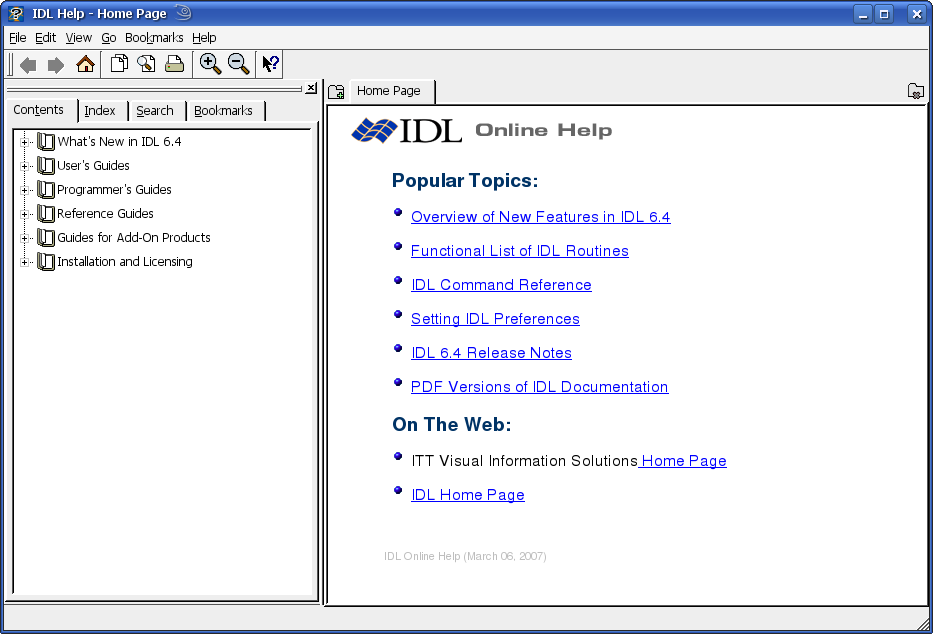
\includegraphics[width=0.8\linewidth]{images/idl_help}
  \end{center}

  The documentation is divided into books aimed at users or developers and
  is fully searchable and cross indexed.

\subsection{Manipulating And Plotting Data}
  Once the data has been loaded from the SDF file we will want to extract
  the specific data we wish to analyse, perhaps perform some mathematical
  operations on it and then plot the results.

  To do this we must learn a few basic essentials about the IDL scripting
  language. Since we are all familiar with the basic concepts shared by
  all computer programming languages, I will just provide a brief overview
  of the essentials and leave other details to the excellent on-line
  documentation.

  IDL supports multidimensional arrays similar to those found in the
  FORTRAN programming language. Whole array operations are supported
  such as \qtt{5*array} to multiply every element of \qtt{array} by $5$.
  Also matrix operations such as addition and multiplication are supported.

  The preferred method for indexing arrays is to use brackets. It is
  possible to use parenthesis instead but this usage is deprecated.
  Column ordering is the same as that used by FORTRAN, so to access
  the $(i,j,k)$th element of an array you would use \qtt{array[i,j,k]}.
  IDL arrays also support ranges so \qtt{array[5:10,3,4]} will return
  a one dimensional array with five elements. \qtt{array[5:*]} specifies
  elements five to $n$ of an $n$ element array. \qtt{array[*,3]} picks
  out the third row of an array.

  There are also a wide range of routines for querying and transforming
  arrays of data. For example, finding minimum and maximum values,
  performing FFTs, etc. These details can all be found by searching the
  on-line documentation. 

  Finally, IDL is a full programming language so you can write your own
  functions and procedures for processing the data to suit your needs.

\subsection{1D Plotting in IDL}
  The most commonly performed plot and perhaps the most useful data analysis
  tool is the 1D plot. In IDL, this is performed by issuing the command
  \cmd{plot,x,y} where \qtt{x} and \qtt{y} are one dimensional arrays of
  equal length. For each element \qtt{x[i]} plotted on the $x$-axis the
  corresponding value \qtt{y[i]} is plotted along the $y$-axis. As a
  simple example:
\begin{boxverbatim}
IDL> plot,[1,2,3],[2,2,5]
\end{boxverbatim}
  Gives rise to the following plot:
  \begin{center}
    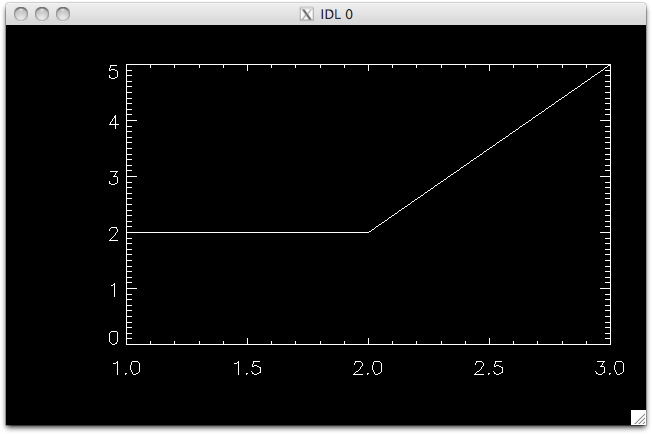
\includegraphics[width=0.7\linewidth]{images/idl_simple_plot}
  \end{center}

  As a more concrete example, we will now take a one-dimensional slice through
  the 2D\linebreak \qtt{Number\_Density} array read in from our SDF data file.
  In this example we will give the $x$ and $y$ axes labels by passing extra
  parameters to the \qtt{plot} routine. A full list of parameters can be found
  in the on-line documentation. In this example we also make use of the
  \qtt{\$} symbol which is IDL's line continuation character.

\begin{boxverbatim}
IDL> data = getdata(0)
IDL> plot,data.x,data.number_density[*,256],xtitle='x', $
IDL>    ytitle='number density'
\end{boxverbatim}
  This command generates the following plot:
  \begin{center}
    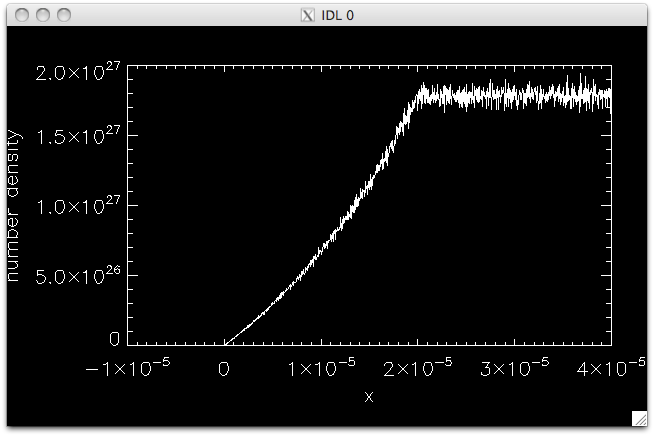
\includegraphics[width=0.7\linewidth]{images/idl_plot}
  \end{center}

\subsection{Postscript Plots}
  The plots shown so far have just been screen-shots of the interactive
  IDL plotting window. These are fairly low quality and could included as
  figures in a paper.

  In order to generate publication quality plots, we must output to the
  postscript device. IDL maintains a graphics context which is set using
  the \cmd{set\_plot} command. The two most commonly used output devices
  are \qtt{x} which denotes the X-server and \qtt{ps} which is the postscript
  device. Once the desired device has been selected, various attributes
  of its behaviour can be altered using the \cmd{device} procedure.
  For example, we can set the output file to use for the postscript plot.
  By default, a file with the name \qtt{idl.ps} is used.

  Note that this file is not fully written until the postscript device is
  closed using the \cmd{device,/close} command. When we have finished our
  plot we can resume plotting to screen by setting the device back to \qtt{x}.

\begin{boxverbatim}
IDL> set_plot,'ps'
IDL> device,filename='out.ps'
IDL> plot,data.x,data.number_density[*,256],xtitle='x', $
IDL>    ytitle='number density',charsize=1.5
IDL> device,/close
IDL> set_plot,'x'
\end{boxverbatim}

  This set of commands results in the following plot being written to
  a file named \qtt{out.ps}.
  \begin{center}
    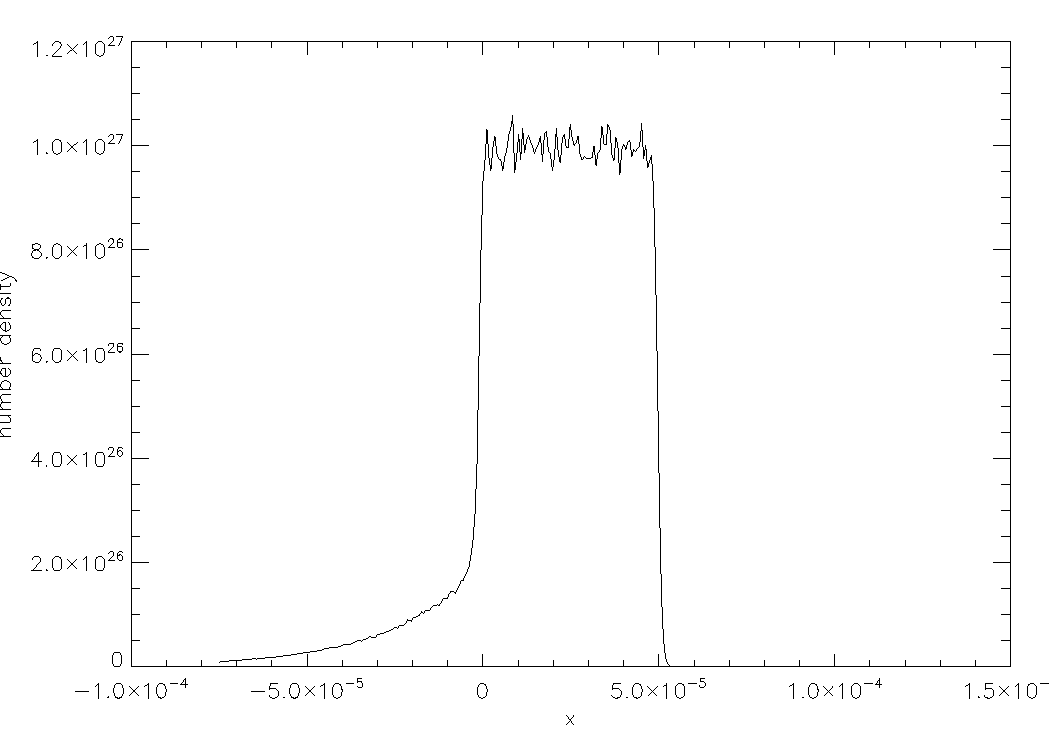
\includegraphics[width=0.8\linewidth]{images/idl_ps_plot}
  \end{center}
  By default, IDL draws its own set of fonts called ``Hershey vector fonts".
  Much better looking results can be obtained by using a postscript font
  instead. These options are passed as parameters to the \cmd{device}
  procedure. More details can be found in the on-line documentation under
  ``Reference Guides $\Rightarrow$ IDL Reference Guide $\Rightarrow$
  Appendices $\Rightarrow$ Fonts".

\subsection{Contour Plots in IDL}
  Whilst 1D plots are excellent tools for quantitive analysis of data,
  we can often get a better qualitative overview of the data using 2D
  or 3D plots.

  One commonly used plot for 2D is the contour plot. The aptly named
  \cmd{contour,z,x,y} procedure takes a 2D array of data values, \qtt{z},
  and plots them against $x$ and $y$ axes which are specified in the
  1D \qtt{x} and \qtt{y} arrays. The number of contour lines to plot is
  specified by the \qtt{nlevels} parameter. If the \qtt{/fill} parameter
  is used then IDL will fill each contour level with a solid colour rather
  than just drawing a line at the contour value.

  The example given below plots a huge number of levels so that a smooth
  looking plot is produced. \qtt{xstyle=1} requests that the $x$ axes drawn
  exactly matches the data in the \qtt{x} variable rather than just using
  a nearby rounded value and similarly for \qtt{ystyle=1}.
\begin{boxverbatim}
IDL> n=100
IDL> levels=max(data.number_density)*findgen(n)/(n-1)
IDL> colors=253.*findgen(n)/(n-1)+1
IDL> contour,data.number_density,data.x,data.y,xstyle=1,ystyle=1, $
IDL>    levels=levels,/fill,c_colors=colors 
\end{boxverbatim}
  Issuing these commands gives us the contour plot shown below. Note that
  the colour table used is not the default one but has been constructed to
  be similar to the one used by VisIt.
  \begin{center}
    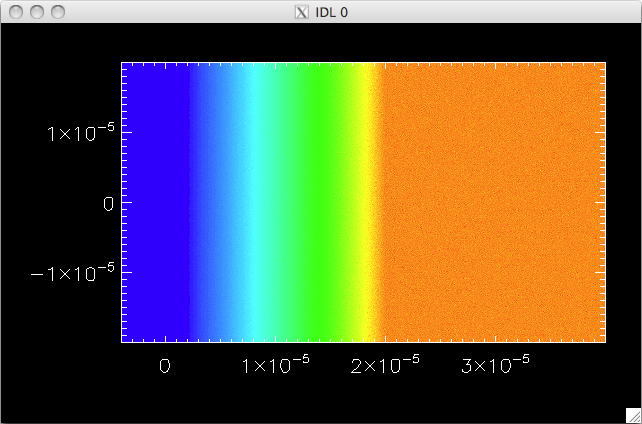
\includegraphics[width=0.8\linewidth]{images/idl_contour}
  \end{center}


\subsection{Shaded Surface Plots in IDL}
  Another method for visualising 2D datasets is to produce a 3D plot in
  which the data is elevated in the $z$ direction by a height proportional
  to its value. IDL has two versions of the surface plot. \cmd{surface}
  produces a wireframe plot and \cmd{shade\_surf} produces a filled and
  shaded one. As we can see from the following example, many of IDL's
  plotting routines accept the same parameters and keywords.

  The first command shown here, \cmd{loadct,3}, asks IDL to load the third
  colour table which is\linebreak ``RED\_TEMPERATURE".

\begin{boxverbatim}
IDL> loadct,3
IDL> shade_surf,data.number_density,data.x,data.y,xstyle=1, $
IDL>    ystyle=1,xtitle='x',ytitle='y',ztitle='number density',charsize=3
\end{boxverbatim}
  \begin{center}
    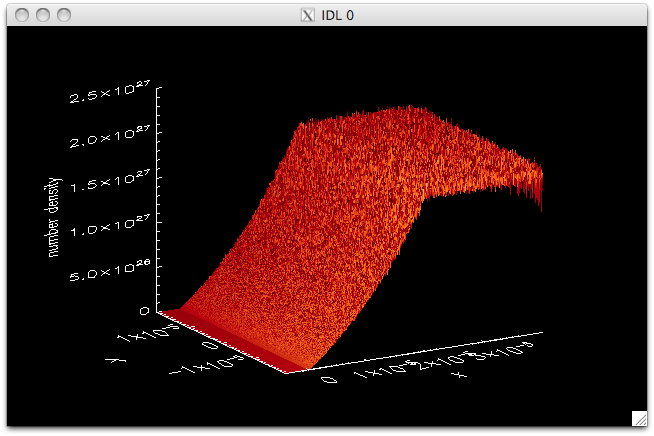
\includegraphics[width=0.8\linewidth]{images/idl_shade_surf}
  \end{center}

\subsection{Interactive Plotting}
  Finally, in recent versions of IDL it is now possible to perform all of
  these plot types in an interactive graphical user interface. The corresponding
  procedures are launched with the commands \cmd{iplot}, \cmd{icontour}
  and \cmd{isurface}.

\begin{boxverbatim}
IDL> iplot,data.x,data.number_density[*,256]
\end{boxverbatim}
  \begin{center}
    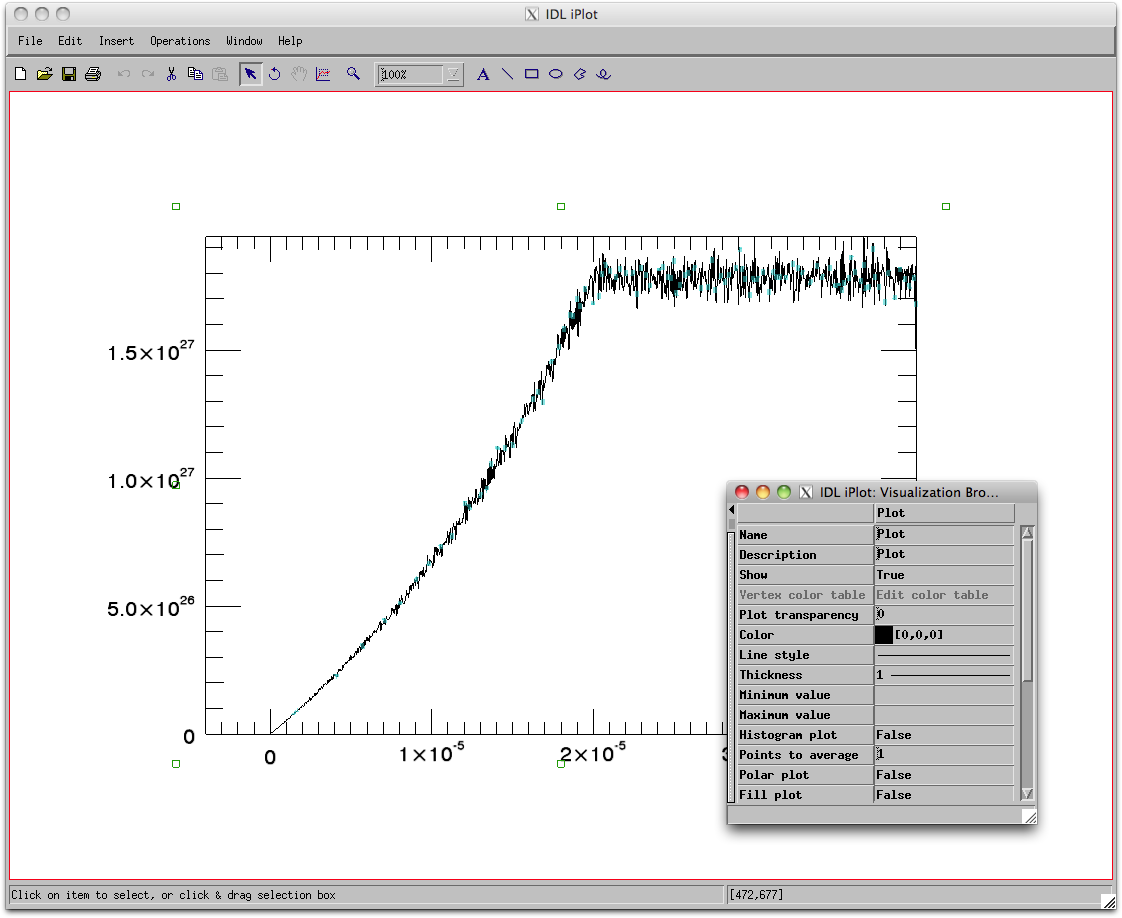
\includegraphics[width=0.8\linewidth]{images/idl_iplot}
  \end{center}

  IDL is an extremely useful tool but it also comes with a fairly hefty
  price tag. If you are not part of an organisation that will buy it for
  you then you may wish to look into a free alternative. It is also a
  proprietary tool and you may not wish to work within the restrictions
  that this imposes.

  There are a number of free tools available which offer similar functionality
  to that of IDL, occasionally producing superior results.

  For a simple drop-in replacement, the GDL project aims to be fully compatible
  and works with the existing {\EPOCH} IDL libraries after a couple of small
  changes. Other tools worth investigating are {\em ``yorick"} and
  {\em ``python"} with the {\em ``SciPy"} libraries. At present there is
  no SDF reader for either of these utilities but one may be developed if
  there is sufficient demand.

\section{Using VisIt to visualise data}

\subsection{LLNL VisIt}
LLNL's VisIt software is a parallel data visualisation package
(\inlinecode{https://wci.llnl.gov/codes/visit/}). {\EPOCH} comes with source
code for the plug-in needed to allow VisIt to load the SDF output files which
are generated by {\EPOCH}. There are full manuals for VisIt which can be
downloaded from the above link so no further details will be given here. To
build the plug-in, first ensure that the visit binary is in the \$PATH
environment variable. Then simply type ``make visit'' in one of the
\inlinecode{epoch\{1,2,3\}d} directories.
For more experienced
users of VisIt, the xml file which is used to generate the plug-in is supplied
in the VisIt subdirectory, called \inlinecode{SDF2.xml}.

  Whilst IDL is an excellent tool for visualising 1D and 2D datasets, it
  is extremely poor when it comes to dealing with 3D data. For this purpose,
  we recommend the use of the {\em ``VisIt"} visualisation tool.

  The other great advantage that VisIt has over IDL is the ability to
  render in parallel, enabling the visualisation of huge datasets which
  IDL would be incapable of dealing with.

  \begin{itemize}
  \item
    Initially developed by the Department of Energy (DOE) Advanced Simulation
    and Computing Initiative (ASCI) 
  \item
    Now developed and maintained by the Lawrence Livermore National Laboratory
    along with a group of external contributors
  \item
    Written in C++ and supports python and Java interfaces
  \item
    Available for UNIX (Irix, Tru64, AIX, Linux, Solaris), Mac OS X
    (10.3, 10.4), and Windows platforms
  \item
    Open source and freely available under the BSD license
  \item
    Plots, operators and database readers are implemented as plugins allowing
    the VisIt to be dynamically extended at run-time
  \item
    Powerful set of tools for manipulating, analysing and visualising 3D
    datasets
  \item
    Parallel and distributed architecture for visualising huge data sets
  \end{itemize}

\subsection{Obtaining And Installing VisIt}
  Both the source code and pre-compiled binaries are available for download
  from the projects web page which is found at the URL
  {\tt https://wci.llnl.gov/codes/visit/home.html}

  \begin{center}
    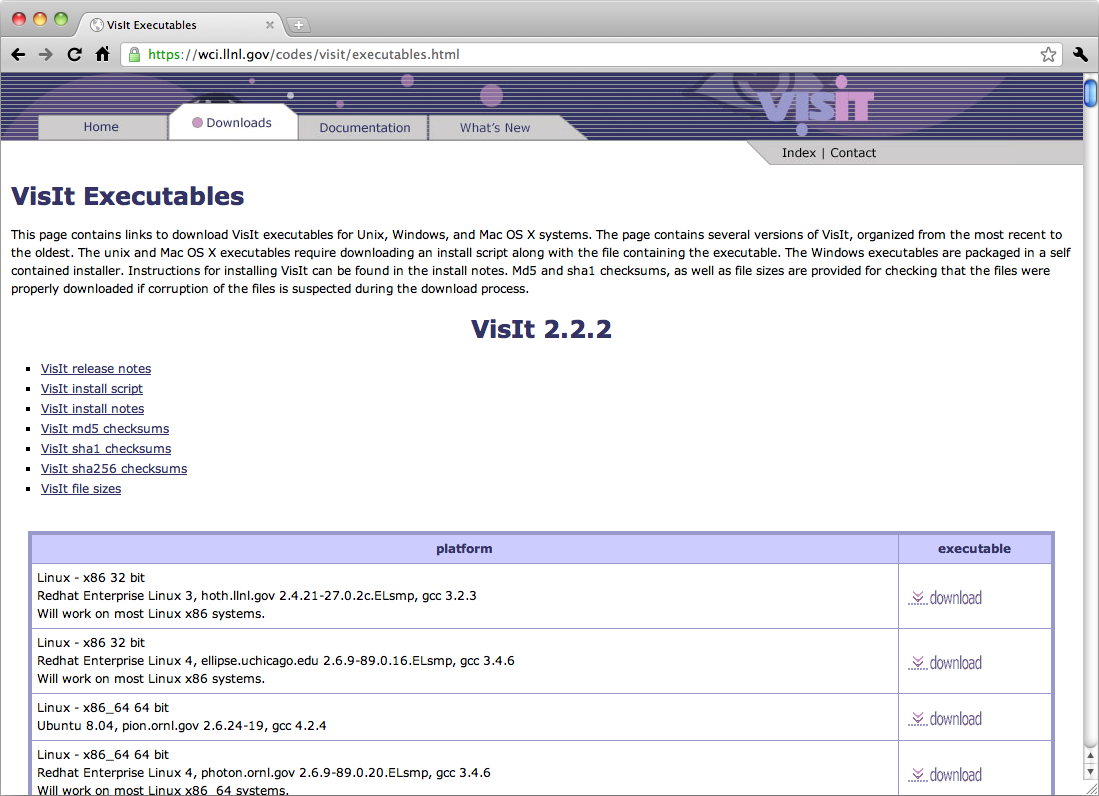
\includegraphics[width=0.8\linewidth]{images/visit_web}
  \end{center}

  There are full instructions for compiling the project from source code
  along with build scripts written to help ease the process. However, this
  is not recommended as it is an extremely large tool and the compilation
  takes hours to complete. It is usually far easier to download a pre-compiled
  binary which matches your system architecture.

  However, occasionally compilation may be a necessary step. Linux
  in particular is a moving target and it is not always possible to
  find a binary which matches the particular combination of libraries
  installed on your system.

  The easiest way to install the VisIt tool is to ask the system
  administrator to do it for you. However, this may not always be the
  best option. The system in question may be run by someone who is
  not concerned with your particular software needs or has insufficient
  skills to deal with the task. In any case, VisIt has a fairly rapid
  release schedule and you may find that some functionality you need
  is not present in the version installed on the machine.

  Fortunately, for all these scenarios it is usually quite easy to install
  a copy in your own home directory. Just find a binary on the web page
  {\tt https://wci.llnl.gov/codes/visit/executables.html} which closely
  matches your machine and download it. This can be unpacked into your
  home directory with the command
  \cmd{tar xzf visit2\_2\_2.linux-x86\_64.tar.gz}. The actual name of
  the file will vary depending on which version you downloaded. This
  will unpack the VisIt binary into a subdirectory named \txt{visit/}.
  Now all that is necessary is to add this to your search path.
  eg. \cmd{export PATH=\$HOME/visit/bin:\$PATH}

  These instructions illustrate the steps required for installing your
  own copy of VisIt when you have no other choice. VisIt is an extremely
  large program, so if a version is already available then it is usually
  better to use the installed version.

  The machines at Warwick have a recent version of VisIt installed which
  is available via the \qtt{modules} system. To make use of it you must
  first issue the command \cmd{module load visit}.

\subsection{Compiling The Reader Plugin}

  One piece of compilation which is almost always necessary is that of
  the SDF reader plugin. This is shipped as source code in a subdirectory
  of the {\EPOCH} repository. It is located in the \txt{VisIt/} subdirectory
  of the main \txt{epoch/} directory. The reader will work for any
  SDF file generated by any code which uses the SDF I/O routines. You do
  not need a separate reader for each version of {\EPOCH}.

  To compile, first navigate to one of the \txt{epoch*d/} directories in your
  {\EPOCH} repository. Just type ``make visit'' and the build scripts should
  take care of the rest.
  The SDF reader plugin will be installed into the directory
  \txt{\$HOME/.visit/linux-intel/plugins/databases/} on your system.
  Note that the \txt{linux-intel/} component will vary depending on
  your machine operating system and architecture.

  Each time you install a new version of VisIt you must recompile the reader
  to match the new installation. It will also occasionally be necessary to
  recompile when changes occur to the SDF data format or the reader plugin
  itself. The developers will notify users if this is the case, although
  it does no harm to regularly recompile the reader as a matter of course.

  We will see later that it is possible to do remote data visualisation
  with VisIt in which the GUI is launched and interacted with on one
  machine and the data files are located on a separate machine entirely.
  In this situation the reader must be installed on the remote machine and
  must match the setup there. The setup on the local machine is unimportant.
  In fact it is not even necessary to have the plugin installed on the
  local machine. This is particularly useful when using a Windows environment
  to analyse data located on a remote UNIX workstation.

\subsection{Loading Data Into VisIt}
  \begin{center}
    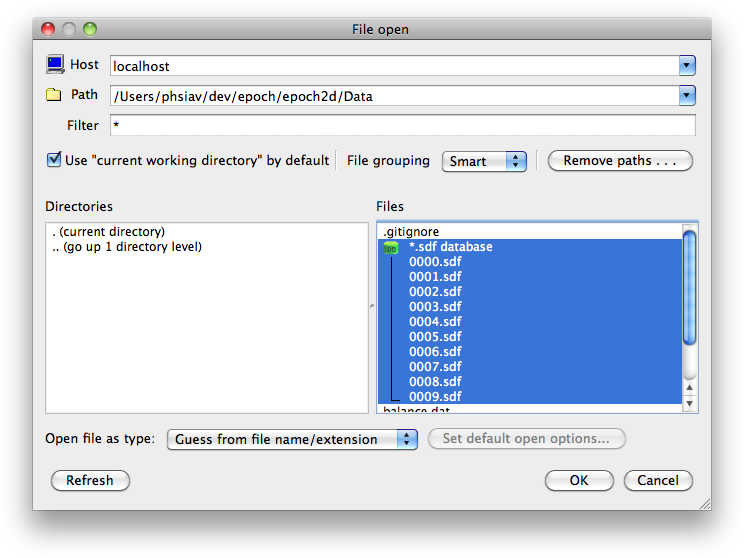
\includegraphics[width=0.8\textwidth]{images/visit_db_list}
  \end{center}

  The most straightforward method for loading data into VisIt is to
  start the application and then browse the filesystem for the dataset
  you are interested in. This is done by selecting \qm{File $\Rightarrow$
  Open file} from the VisIt menu bar. A file selection dialogue will appear
  allowing you to browse directories along with the options to filter
  the results according to a given regular expression and grouping options.
  By default, VisIt will attempt to group all files containing the same
  suffix and some kind of numbering system into a sort of virtual database.

  The right-hand pane of this window shows a list of selected files which
  will appear in the main VisIt window when you are finished.

  An alternative method of specifying the data file to open is to pass
  a command line option when the tool is launched. An example of this
  method is \cmd{visit -o Data/0000.sdf}. When the file is specified in
  this manner the list of files shown in the VisIt window will also
  include the full list of files in the dataset's subdirectory and
  all the files in the current working directory. The other SDF files
  will be grouped together in a virtual database.

  Yet another method for selecting the dataset to use is by opening a
  previously saved session file. Will discuss this further in a later section

  \begin{center}
    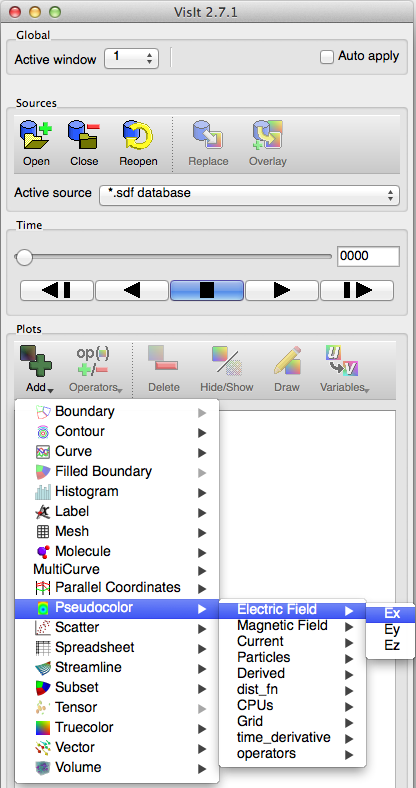
\includegraphics[height=0.7\textheight]{images/visit_select_var}
  \end{center}
  Once a SDF file has been successfully loaded the \qm{Add} menu item
  will become un-greyed and the cycle numbers for each file in the virtual
  database will be displayed. If we navigate to one of the plot types we
  are able to select the variable to plot from a drop-down list.

\subsection{Contour Plots in VisIt}
  We will now replicate each of the plots which we generated using IDL
  in earlier sections. For reasons which will soon become clear we begin
  with the contour plot and move on to the 1D plot in the next section.

  Having opened the same dataset we were using in the IDL discussion we
  now select the \qm{Add} menu item. Notice that many of the plot
  types listed here are greyed out and cannot be selected. This is because
  many of the plots are dependent on the type or dimensionality of the
  variable to be plotted. If our dataset contains no variables which match
  the required properties for a plot, the plot menu will be disabled.

  For the current dataset there is no \qm{Boundary} plot available since this
  requires multi-material data and none of our variables meet
  that criteria.

  The list contains a menu item for a \qm{Contour} plot. We are not going
  to select this item since it only generates a contour plot with lines
  indicating each contour level and not a filled version. Instead we
  choose \qm{Add $\Rightarrow$ Pseudocolor $\Rightarrow$ Derived $\Rightarrow$
  Number\_Density} and then hit the \qm{Draw} button.
  \begin{center}
    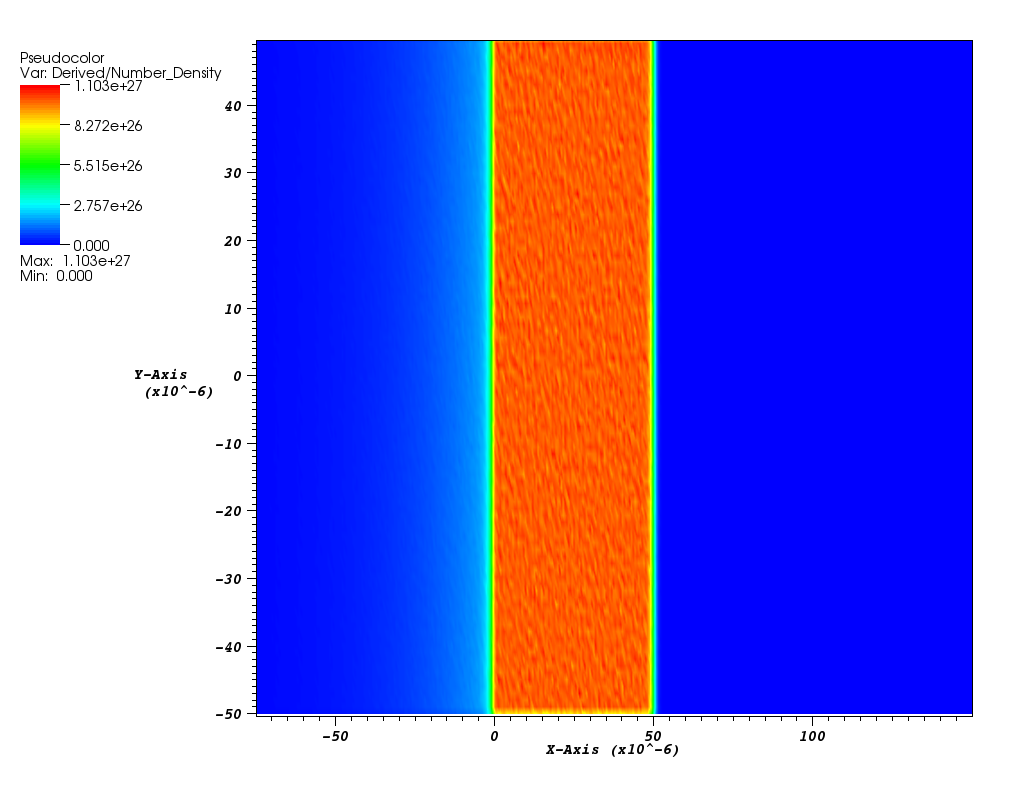
\includegraphics[width=0.8\linewidth]{images/visit_contour}
  \end{center}

  There are many settings which can alter the visual appearance
  of plots generated by VisIt. The first point of call is usually to
  open up the \qm{Plot Attributes} or \qm{Operator Attributes} dialogue
  corresponding to the
  plot in question. A simpler method for accomplishing this task is
  to double-click on the plot in the main VisIt menu pane which will
  launch the corresponding \qm{Plot Attributes} dialogue.

  If it is the operator attributes you wish to change,
  click on the white arrow on the left hand side of the plot in the
  main VisIt menu pane. This will drop down to reveal a list containing
  the plot and all operators acting on it. Double-clicking on an operator
  will launch the corresponding \qm{Operator Attributes} dialogue.
  \begin{center}
    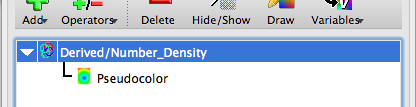
\includegraphics[width=0.7\linewidth]{images/visit_attrib}
  \end{center}

  Another important tool for controlling the appearance of plots can
  be found in \qm{Controls $\Rightarrow$ Annotation} from the VisIt menu
  bar. This allows all of the plot annotations to be modified such as
  the legend, title, axis labels, etc.
  \begin{center}
    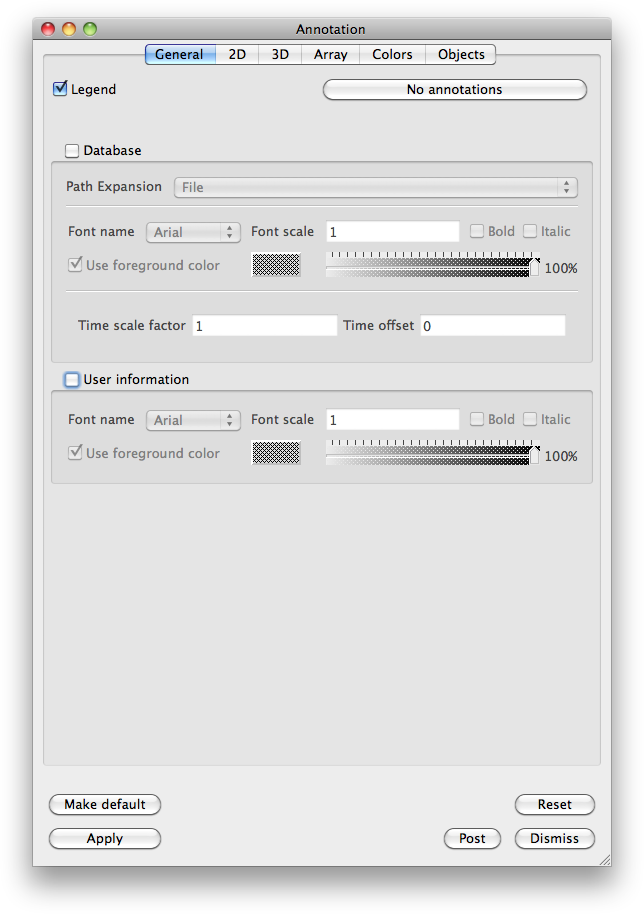
\includegraphics[width=0.6\linewidth]{images/visit_annot}
  \end{center}

\subsection{1D Plotting in VisIt}
  A 1D plot in VisIt is called a \qm{Curve} plot. We already mentioned that
  this was greyed out because we have no one dimensional variables in our
  data file.

  The solution to this dilemma is the lineout operator which extracts a
  one dimensional array from a 2D or 3D variable. This operator is selected
  by pressing the button with red and blue lines located at the top of
  the plot window.
  \begin{center}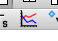
\includegraphics{images/visit_lineout}\end{center}

  Once the button has been pressed, we can click and drag anywhere in
  the \qm{Pseudocolor} plot window. When we release the mouse button a
  new plot window pops up containing a \qm{Curve} plot of the data just
  selected.
  \begin{center}
    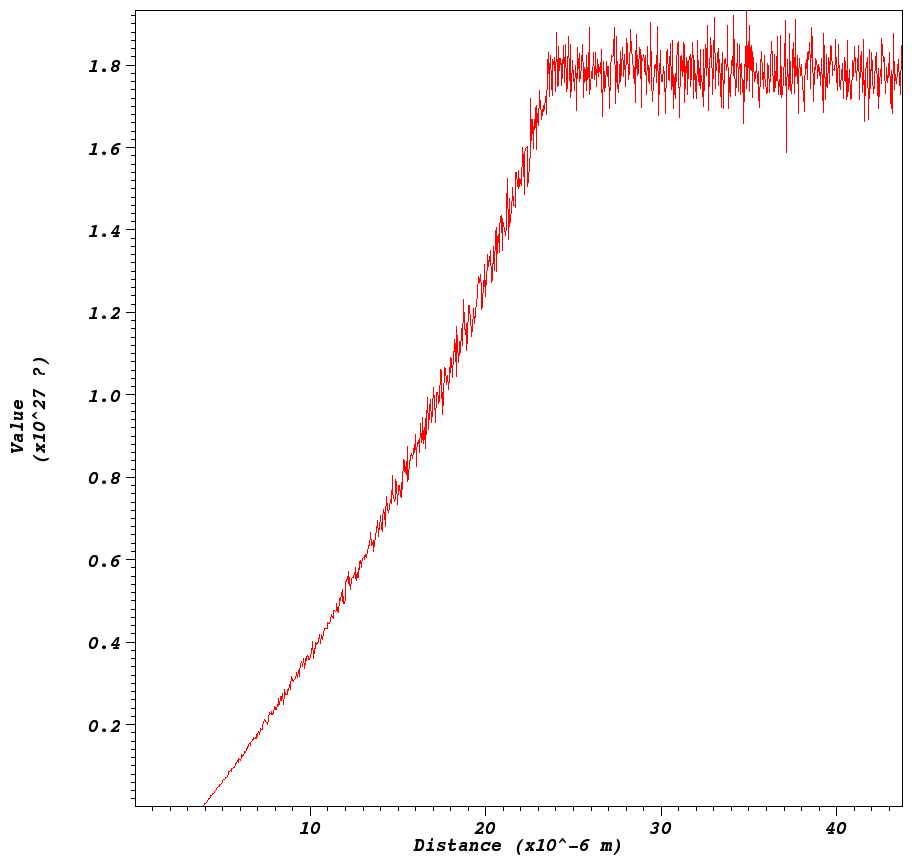
\includegraphics[width=0.8\linewidth]{images/visit_curve}
  \end{center}

  In order to change the attributes for this plot, we must first select
  \qm{Active window} number 2 in the main VisIt pane.

\subsection{Shaded Surface Plots in VisIt}
  Again, we will confusingly refuse to pick the obvious plot type for this
  task. There is \qm{Surface} plot listed in the menu. However, most of the
  time the \qm{Elevator} operator does what we want and also gives us more
  flexibility.

  The first step is to do a \qm{Pseudocolor} plot of \qm{Number\_Density} as
  we did before. Next select the \qm{OpAtts $\Rightarrow$ Elevate} menu item.
  In the pop up dialogue click on the \qm{Elevation height relative to XY
  limits} and then \qm{Apply}. Click \qm{Yes} when the warning dialogue pops
  up.
  \begin{center}
    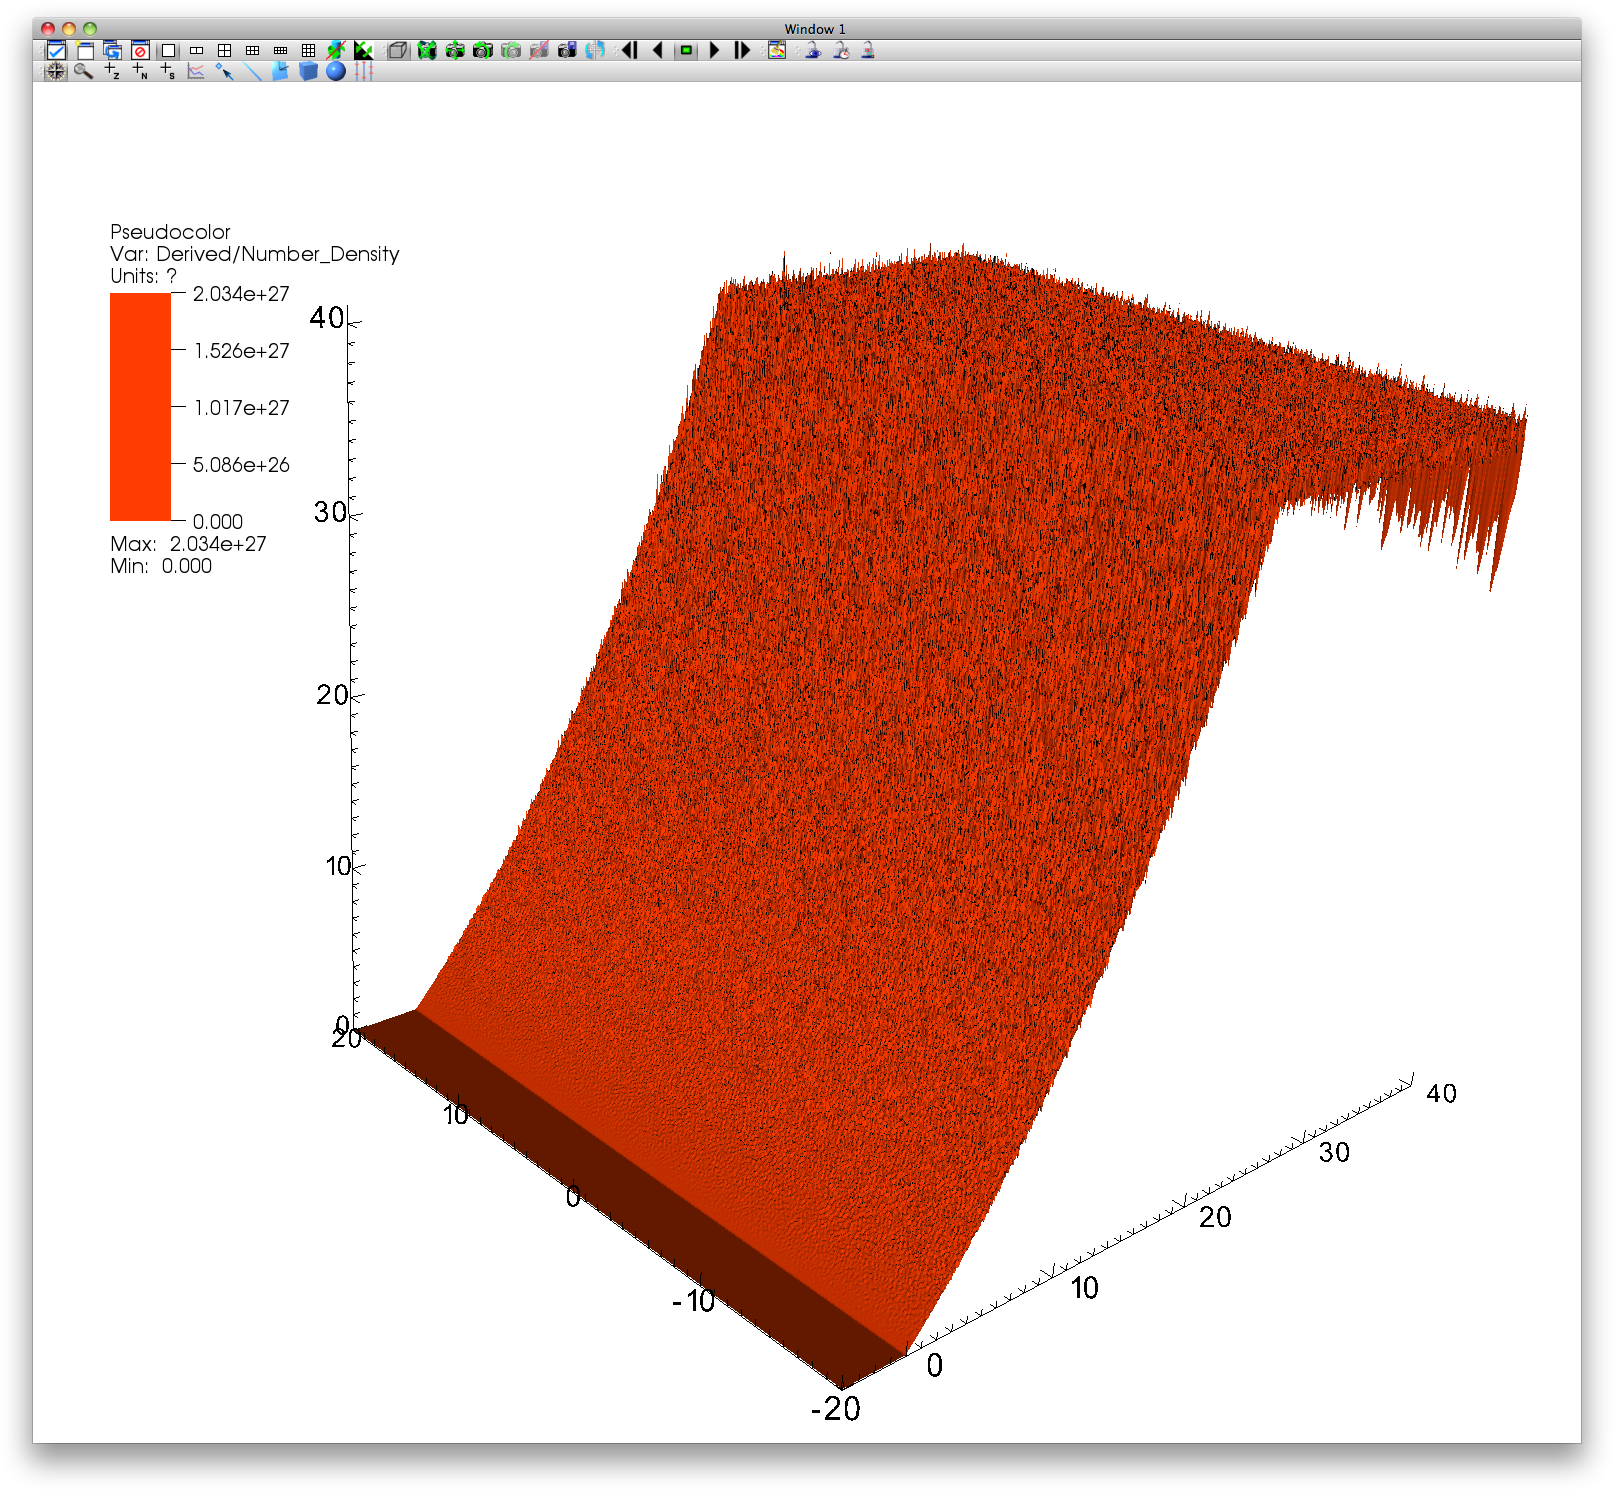
\includegraphics[width=0.8\linewidth]{images/visit_shade_surf}
  \end{center}

  To make this plot look similar to the one generated by IDL, we have changed
  the colour table using \qm{Controls $\Rightarrow$ Color table}.
  We also changed the axis appearance with the annotations menu discussed
  earlier and changed the height of the elevation using the min and max
  operator attributes.

\subsection{Creating User-Defined Expressions}
  VisIt comes with an extremely powerful method of manipulating data before
  visualising the results. The basic idea is that an array is transformed
  by applying a set of mathematical functions on all its elements and then
  the result is defined as a new variable. Once defined, this variable
  behaves in exactly the same way as any of the variables read from the
  data file.

  As an example, we can combine the three components of electric field
  to generate a single electric field vector.
  \begin{center}
    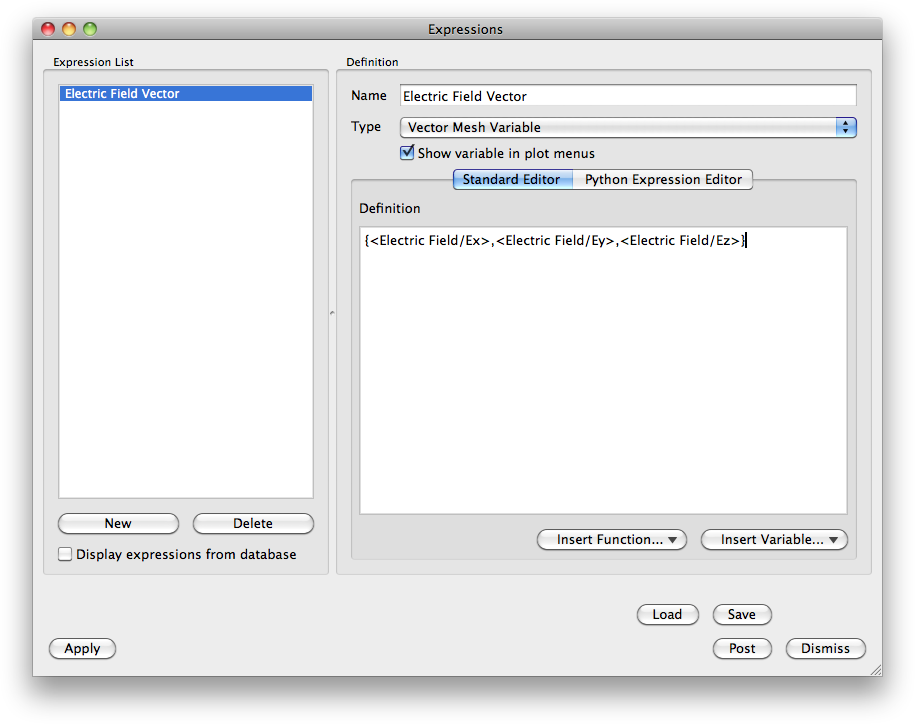
\includegraphics[width=0.8\linewidth]{images/visit_expression_vector}
  \end{center}

  Now when we return to the \qm{Add} menu we see that the \qm{Vector}
  and \qm{Streamline} plot types now have an entry for our newly defined
  vector.

\subsection{Creating Movies}
  A compelling visualisation of numerically generated data is often made
  by combining a series of images into a movie. This can be an invaluable
  method for illustrating the basic behaviour of a system as it changes
  over time. Alternatively rotating around a 3D scene can sometimes
  give a much better idea of the structure in the model being presented. 
  There can also be much to gain by constructing visual fly-throughs
  of a scene, dynamically slicing through sets of data or combinations
  of all these techniques.

  VisIt provides several facilities for generating movies from your
  data. The simplest of these is to select the \qm{File $\Rightarrow$
  Save movie} menu item. This pops up a movie wizard which will walk
  you through the process of generating a simple linear movie based
  on the time-advancing snapshots represented by your virtual database
  of files. Alternatively you can select one of the pre-defined movie
  templates which manipulate the currently selected plot and create
  a movie from that.

  Creating a simple time advancing movie is as simple as walking through
  the wizard dialogue and selecting from the self-explanatory options
  presented to you.

  For many uses, the wizard will give exactly the desired results. However
  it is occasionally useful to have a little more control over how the
  movie is created. In such cases it can be useful to specify an image
  format such as \qm{PNG} to save to rather than \qm{MPEG}. VisIt will
  then generate one image per frame and number them consecutively. At
  the end of the process the images can be converted into a movie using
  whatever tool best accomplishes the task.

  \begin{center}
    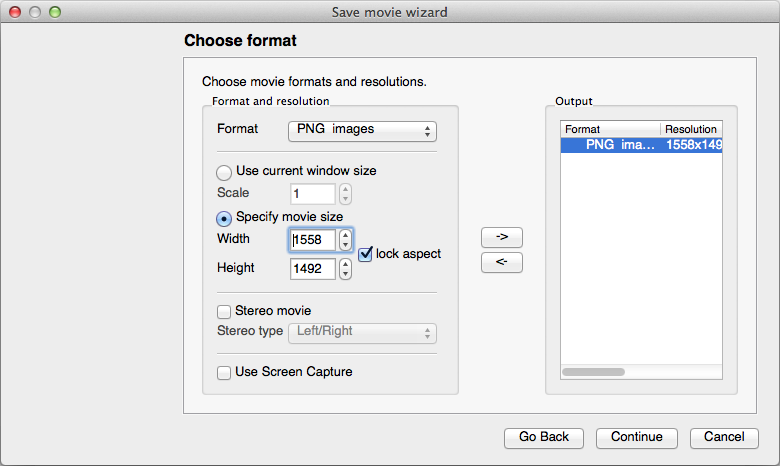
\includegraphics[width=0.8\linewidth]{images/visit_movie}
  \end{center}
  Another useful tip is to select the \qm{Later, tell me the command to
  run} radio button. This will output a long command which can run from
  a UNIX terminal screen. The advantage is that no X session is required
  so the command can be run in the background. It also becomes a simple
  task to interrupt the job at any point and resume it from where it
  left off at a later date. In a similar manner it is easy to resume
  a job which crashes half way through for any reason.

  More complex movies can be created by using VisIt's keyframing facility
  which allows you to change animation attributes such as view or plot
  attributes as the animation progresses. Further information about this
  somewhat complex task can be found in the on-line help.

  Finally, you can use VisIt's python scripting interface to programmatically
  describe the details of each frame as the movie progresses. This approach
  offers far more flexibility in what can be achieved but is also much
  more involved and time consuming than the previous two methods. Again,
  further information on this subject can be found in the on-line help
  system.

\subsection{Remote Visualisation}
  It was mentioned earlier that it is possible to perform remote visualisation
  using VisIt. This is a process in which the data files being interrogated
  reside on a different machine to the one on which the VisIt GUI runs and
  where the results are plotted.

  This method of working can be extremely useful when the data is generated
  on a powerful machine located in an external environment such as a large
  cluster. Another common use is when {\EPOCH} is executed on a UNIX machine
  and the desktop used for visualisation is running Windows.

  It is sometimes possible to run a graphical tool on the remote machine
  and tunnel the X-server session through to the local machine but this
  can be quite slow and unstable. When connecting to a remote VisIt
  instance the only data which needs to be sent between machines is the
  pre-rendered image and a few simple plotting commands. Naturally, this
  can be a {\em much} faster approach.

  Also, as mentioned before, it is possible to use a machine on which the
  reader plugin is difficult or impossible to compile for and connect
  to a machine on which the reader is already installed.

  In order to use the remote visualisation facility, you must first
  set up a \qm{Host Profile} for the remote machine using the \qm{Options
  $\Rightarrow$ Host Profiles} menu item. The pre-compiled binaries are
  shipped with a long list of pre-defined host profiles. These are unnecessary
  for anyone not affiliated and can safely be removed by deleting the
  directory \txt{\$HOME/visit/current/.visit/} (assuming you have unpacked
  the VisIt tarball into your home directory).

  \begin{center}
    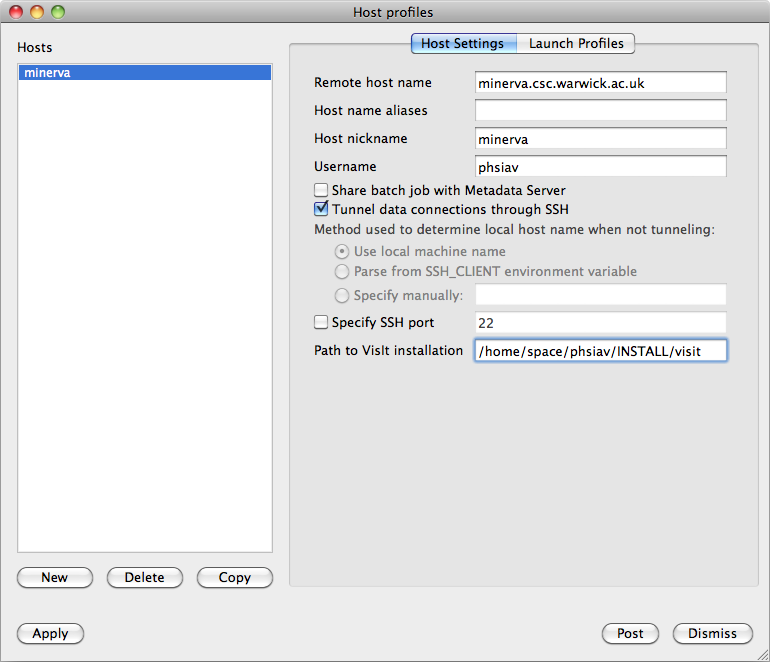
\includegraphics[width=0.8\linewidth]{images/visit_host_profile}
  \end{center}

  Create a new profile by clicking on the \qm{New profile} button and filling
  out some of the form fields. The important ones to change are \qm{Profile
  name}, \qm{Remote host name}, \qm{Host name aliases} and \qm{Username}.
  If the visit binary is not in your default search path on the remote
  machine then you must specify its location by passing \qm{-dir
  /base/installpath/visit} to \qm{Additional options}.

  Now select the \qm{Options $\Rightarrow$ Save Settings} menu item to
  ensure that the profile is saved for future sessions.

  Data on the remote machine can now be loaded by selecting \qm{File
  $\Rightarrow$ Open file} and picking the desired host profile
  from the drop down list of \qm{Hosts}. VisIt will wait for the
  remote process to launch and then continue with the file selection
  procedure but now displaying files located on the remote machine
  rather than the local one. From this point on everything should work
  as before except you should see the name of the remote machine in the
  \qm{Selected files} dialogue. 

  \begin{center}
    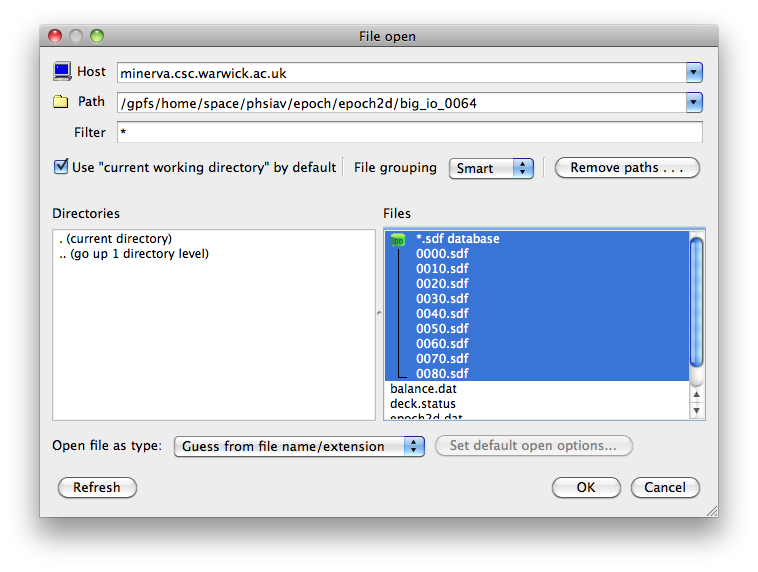
\includegraphics[width=0.8\linewidth]{images/visit_host_files}
  \end{center}

\subsection{Parallel Visualisation}
  Before reading this section be warned that the current version of
  the SDF reader is not capable of reading data in parallel! However,
  this is high on the list of issues to be addressed so a parallel
  version ought to be released some time in the near future.

  Parallel visualisation is performed in almost exactly the same manner
  as remote visualisation. Again, you must create a host profile for the
  purpose except this time you need to check the \qm{Parallel computation
  engine} radio button. This will activate a \qm{Parallel options} tab
  which must be filled in to match the cluster on which the job will
  be launched.

  The major difference now is due to the fact that VisIt must be launched
  by an external job script which fits in with the queueing system used
  by the parallel machine. Usually you will need to consult with the
  system administrator of the cluster to confirm which launch method and
  arguments to use.

  The details of job launch can be better understood by reading through
  the file\linebreak \txt{\$HOME/visit/current/bin/internallauncher}. This is
  a bash script which parses the arguments and executes the specified
  launch method.
%\subsection{Examples}
%  \begin{itemize}
%  \item
%  \end{itemize}
%\section*{Summary}
%
%\begin{frame}{Summary}
%
%  % Keep the summary *very short*.
%  \begin{itemize}
%  \item
%    Item 1
%  \end{itemize}
%\end{frame}



\appendix
\section{Changes between version 3.1 and 4.0}

\subsection{Changes to the Makefile}

Some changes have been made to the Makefile. These are documented in
\sect{makefile}.\\

\noindent The following compile-time defines have been added to the Makefile:
\begin{itemize}
\item NO\_IO
\item PARTICLE\_ID
\item PARTICLE\_ID4
\item COLLISIONS\_TEST
\item PHOTONS
\item TRIDENT\_PHOTONS
\item PREFETCH
\end{itemize}
\bigskip

\noindent The following compile-time defines have been removed from the
   Makefile:
\begin{itemize}
\item COLLISIONS
\item SPLIT\_PARTICLES\_AFTER\_PUSH
\item PARTICLE\_IONISE
\end{itemize}

\subsection{Major features and new blocks added to the input deck}

\begin{itemize}
\item CPML boundary conditions - See \sect{cpml}
\item Thermal boundary conditions - See \sect{thermal}
\item Collisions - See \sect{collisions_block}
\item QED - See \sect{qed_block}
\item Subsets - See \sect{subset_block}
\item Ionisation - See \sect{ionisation}
\item Single-precision output - See \sect{single_precision_output}
\item Multiple output blocks - See \sect{multiple_output}
\item Particle migration - See \sect{migration}
\end{itemize}
%dumpmask - single, average_single

\subsection{Additional output block parameters}

The following parameters have also been added to the ``output'' block
(see \sect{output_directives}):

\begin{itemize}
\item dump\_first
\item dump\_last
\item force\_first\_to\_be\_restartable
\item ejected\_particles
\item absorption
\item id
\item name
\item restartable
\end{itemize}

\subsection{Other additions to the input deck}

\begin{itemize}
\item npart\_per\_cell - See \sect{species_block}
\item dir\_\{xy,yz,zx\}\_angle - See \sect{dist_fn_block}
\item particle\_tstart - See \sect{control_block}
\item identify - See \sect{species_block}
\end{itemize}

Finally, the input deck now has a method for writing continuation lines.
If the deck contains a ``\textbackslash'' character then the rest of the line
is ignored and the next line becomes a continuation of the current one.


\section{Changes between version 4.0 and 4.3}

\subsection{Changes to the Makefile}

Some changes have been made to the Makefile. These are documented in
\sect{makefile}.\\

\noindent The following compile-time define has been added to the Makefile:
\begin{itemize}
\item MPI\_DEBUG
\end{itemize}
\bigskip

\noindent The following compile-time define has been removed from the Makefile:
\begin{itemize}
\item FIELD\_DEBUG
\end{itemize}


\subsection{Additions to the input deck}
The following parameters have been added to the ``control'' block of
the input deck (see \sect{control_block}):
\begin{itemize}
\item nproc\{x,y,z\}
\item smooth\_currents
\item field\_ionisation
\item use\_exact\_restart
\item allow\_cpu\_reduce
\item check\_stop\_file\_frequency
\item stop\_at\_walltime
\item stop\_at\_walltime\_file
\item simplify\_deck
\item print\_constants
\item The ``restart\_snapshot'' parameter now accepts filenames
\end{itemize}
\bigskip

\noindent The following parameters have been added to the ``output'' block of
the input deck (see \sect{output_block}):
\begin{itemize}
\item disabled
\item time\_start
\item time\_stop
\item nstep\_start
\item nstep\_stop
\item dump\_at\_times
\item dump\_at\_nsteps
\item dump\_cycle
\item dump\_cycle\_first\_index
\item filesystem
\item file\_prefix
\item rolling\_restart
\item particle\_energy
\item relativistic\_mass
\item gamma
\item total\_energy\_sum
\item optical\_depth
\item qed\_energy
\item trident\_optical\_depth
\item The default value of ``dump\_first'' is now ``T''
\end{itemize}
\bigskip

\noindent The following parameter has been added to the ``collisions'' block of
the input deck (see \sect{collisions_block}):
\begin{itemize}
\item collisional\_ionisation
\end{itemize}
\bigskip

\noindent The following parameter has been added to the ``qed'' block of
the input deck (see \sect{qed_block}):
\begin{itemize}
\item use\_radiation\_reaction
\end{itemize}
\bigskip

\noindent The following parameter has been added to the ``species'' block of
the input deck (see \sect{species_block}):
\begin{itemize}
\item immobile
\end{itemize}
\bigskip

\noindent The following parameters were changed in the ``laser'' block of
the input deck (see \sect{laser_block}):
\begin{itemize}
\item The ``phase'' parameter can now be time varying
\item The ``profile'' parameter can now be time varying
\end{itemize}
\bigskip

\noindent The following parameters have been added to the list of pre-defined
constants (see \sect{constants}).
\begin{itemize}
\item nproc\_\{x,y,z\}
\item nsteps
\item t\_end
\item cc
\end{itemize}
\bigskip

\noindent There has also been a new ``output\_global'' block added to the
input deck. This is documented in \sect{output_global_block}.

\subsection{Changes in behaviour which are not due to changes in the input deck}
\begin{itemize}
\item The species ``drift'' property is now applied to particles whilst the
  moving window model is active. In previous versions of the code, this
  property was ignored once the moving window began.
\item Ionisation species now inherit their ``dumpmask''. See \sect{ionisation}
  for details.
\item Default values for ignorable directions were added.
   This change allows submitting 3D or 2D input decks to a 1D
   version of {\EPOCH} and 3D input decks to a 2D version of {\EPOCH}.
   Any references to y/z will be set equal to zero unless overridden
   by a deck constant. Other y/z values also assume sensible
   defaults, eg. 1 grid cell, 1 metre thick, etc.
\item Automatic byte swapping is carried out by the SDF library.
   The library now checks the endianness of the SDF file and
   byte-swaps the data if required.
\item ``qed'' blocks may now be present even if the code was not compiled
   using the ``-DPHOTONS'' flag.
   The code will only halt if ``use\_qed=T'' inside the ``qed'' block.
\item The code now checks for the Data directory in a file named
   ``USE\_DATA\_DIRECTORY'' before prompting at the command-line. This allows
   the code to be run without waiting for input at the command-line.
\item The field and particle grids are now automatically written to SDF output
   files if they are needed.
\item The Data directory may now contain a `\verb|/|' character.
\end{itemize}


\section{Changes between version 4.3 and 4.8}

\subsection{Changes to the Makefile}

Some changes have been made to the Makefile. These are documented in
\sect{makefile}.\\

\noindent The following compile-time define has been added to the Makefile:
\begin{itemize}
\item PER\_SPECIES\_WEIGHT
\item NO\_TRACER\_PARTICLES
\item NO\_PARTICLE\_PROBES
\item PARSER\_CHECKING
\end{itemize}
\bigskip

\noindent The following compile-time define has been removed from the Makefile:
\begin{itemize}
\item PER\_PARTICLE\_WEIGHT
\item TRACER\_PARTICLES
\item PARTICLE\_PROBES
\end{itemize}


\subsection{Additions to the input deck}
The following parameters have been added to the ``control'' block of
the input deck (see \sect{control_block}):
\begin{itemize}
\item allow\_missing\_restart
\item print\_eta\_string
\item n\_zeros
\end{itemize}
\bigskip

\noindent The following parameters have been added to the ``output'' block of
the input deck (see \sect{output_block}):
\begin{itemize}
\item weight (synonym for particle\_weight)
\end{itemize}
\bigskip

\noindent The following parameters have been added to the ``output\_global''
block of the input deck (see \sect{output_global_block}):
\begin{itemize}
\item dump\_first\_after\_restart
\end{itemize}
\bigskip

\noindent The following parameters have been added to the ``subset'' block of
the input deck (see \sect{subset_block}):
\begin{itemize}
\item skip, skip\_{x,y,z}
\end{itemize}
\bigskip

\section{Changes between version 4.8 and 4.9}

\subsection{New capabilities}
Version 4.9 adds significant new capabilities as follows:

\begin{itemize}
\item delta-f version: particle distributions can be expressed as
   $f_0 + f_1$ where $f_0$ is a specified background plasma and all simulation
   particles are used to describe the $f_1$ component, documented in
   \sect{deltaf}.
\item selectable field solvers: 3 new solvers have been added for fields, fully
   documented in \sect{maxwell_solvers}.
\end{itemize}
\bigskip

\subsection{Changes to the Makefile}

Some changes have been made to the Makefile. These are documented in
\sect{makefile}.\\

\noindent The following compile-time define has been added to the Makefile:
\begin{itemize}
\item DELTAF\_METHOD
\end{itemize}
\bigskip

\subsection{Additions to the input deck}

The following alterations were made to the input deck:
\begin{itemize}
\item ioniz* (with a ``z'') aliases have been added for ionis* keywords.
\item y and z parameters can now appear in the input deck in EPOCH 1D and 2D.
\end{itemize}
\bigskip

A new deck block has been added. The particles\_from\_file block allows loading
of custom particle data from raw binary data files. See
\sect{particles_from_file} for details.
This block accepts the following parameters:
\begin{itemize}
\item species
\item \{xyz\}\_data
\item w\_data
\item \{xyz\}\_data
\item id\{4,8\}\_data
\item offset
\end{itemize}
\bigskip

\noindent The following parameters have been added to the ``control'' block of
the input deck (see \sect{control_block}):
\begin{itemize}
\item maxwell\_solver
\item use\_current\_correction
\end{itemize}
\bigskip

\noindent The following parameters have been added to the ``species'' block of
the input deck (see \sect{species_block}):
\begin{itemize}
\item maxwell\_solver
\item density\_back
\item drift\_\{x,y,z\}\_back
\item temp\_\{x,y,z\}\_back
\item temp\_\{x,y,z\}\_back\_ev
\item temp\_back
\item temp\_back\_ev
\end{itemize}
\bigskip

\noindent The following parameters have been added to the ``dist\_fn' block of
the input deck (see \sect{dist_fn_block}):
\begin{itemize}
\item dir may now take the value mod\_p
\item restrict\_mod\_p
\end{itemize}

\subsection{Changes not resulting from changes to the deck}
\begin{itemize}
\item Lasers can be specified with time-varying frequency profile.
\item The existing subset blocks can now be applied to field and derived grid
  variables. If spatial restrictions are used, subsections will be output,
  along with a corresponding grid.
  Note that these are not compatible with the ``skip'' parameter to subset
  blocks.
\item The dist\_fn block ``range'' keyword is now respected for spatial
  directions, allowing a spatial subset of the distribution function to be
  output directly.
\item Some corrections were applied to calculation of thermal boundary
  conditions for particles.
\item The load balancer may now be disabled by setting a 0 or negative
  threshold.
\end{itemize}
\bigskip


\section{Changes between version 4.9 and 4.10}

\subsection{New capabilities}
Version 4.10 adds the following new capabilities:

\begin{itemize}
\item Time varying particle injectors. See \sect{injector_block}
\item Per-species particle boundaries. You can now specify bc\_x\_min and
   bc\_x\_max to a species block. This overrides the global boundaries for that
   species. See \sect{per_species_bcs}
\item Added ``particles\_per\_cell'' output diagnostic.
   See \sect{output_directives}
\end{itemize}
\bigskip


\section{Changes between version 4.10 and 4.11}

\subsection{New capabilities}
Version 4.11 adds the following new capabilities:

\begin{itemize}
\item Added time dependent moving window. No new input deck parameters have
    been added, but it is now possible to specify ``window\_v\_x'' to be a
    function that varies in time. See \sect{window_block}
\item If ``print\_constants=T'' in the control block (see \sect{control_block})
    deck constants are now output to a separate file named ``const.status''.
    This allows for easier post-processing.
\item Added COMPILER=auto option to automatically detect compiler. See
    \sect{makefile}
\end{itemize}

The following correction has been made:
\begin{itemize}
\item Fractional numbers of particles-per-cell now function as expected when
used in conjunction with the moving window.
\end{itemize}
\bigskip


\section{Changes between version 4.11 and 4.12}

\subsection{New capabilities}
Version 4.12 adds the following new capabilities:

\begin{itemize}
\item Added ``average\_weight'' output diagnostic.
    See \sect{output_directives}
\item Removed the ``PARTICLE\_COUNT\_UPDATE'' Makefile flag and replaced
    it with a\linebreak ``use\_particle\_count\_update'' parameter in the
    control block. See \sect{control_block}
\item Added ``use\_flux\_maxwellian'' option to the ``injector'' block.
    See \sect{injector_block}
\item Added ``lehe\_\{x,y,z\}'' flags to the ``maxwell\_solver'' option in
    the control block. See \sect{control_block}
\item Added ``custom'' flag to the ``maxwell\_solver'' option in
    the control block. See \sect{control_block} and \sect{stencil_block}
\item Added the ``WORK\_DONE\_INTEGRATED'' Makefile flag and corresponding
    dumpmask directives ``work\_\{x,y,z\}'' and ``work\_\{x,y,z\}\_total''.
    These add a diagnostic for the work done on a particle by the electric
    field. See \sect{makefile} and \sect{output_directives}.
\item Added the ``use\_accurate\_n\_zeros'' flag to the control block.
    See \sect{control_block}
\end{itemize}
\bigskip


\section{Changes between version 4.12 and 4.14}

\subsection{New capabilities}
Version 4.14 adds the following new capabilities:

\begin{itemize}
\item Added the ``reset\_walltime'' flag to the control block.
    See \sect{control_block}
\item Changed the default value of ``print\_eta\_string'' to ``T'' in the
    control block.
\end{itemize}
\bigskip


\section{Simple binary files}
\label{sec:binaryfile}
There are several input deck blocks which can read conditions directly from
a user-specified file. These include the \sectit{fields_block},
\sectit{species_block} and \sectit{particles_from_file}. In all such cases,
the files specified must be in a simple binary format, often referred to
as ``raw'' binary files.

Binary files are machine readable, but not human readable. If you try opening
a binary file in a text editor then you will see incomprehensible characters
and some text editors might even crash. Most languages can write binary files,
see ``writeu'' (in IDL/GDL), ``fwrite'' in MatLab, the ``b'' parameter to
``open'' in Python and ``form='UNFORMATTED' '' in Fortran, so please see the
documentation for those languages. Note that standard unformatted output in
Fortran also writes some additional hidden output to the file that alters the
offset of the actual binary array data within the file. It is therefore
recommended that you always use the ``access='STREAM' '' modifier whenever
writing such files from Fortran programs.

For illustration purposes, here is a simple example of writing a 2D array
to file using Fortran:
\begin{boxverbatim}
PROGRAM output_array

  INTEGER :: iu, istat
  INTEGER, PARAMETER :: nx = 10, ny = 20
  DOUBLE PRECISION :: array(nx,ny)
  CHARACTER(LEN=*), PARAMETER :: filename = 'array.dat'

  array = 2.0d0

  OPEN(newunit=iu, file=filename, status='NEW', form='UNFORMATTED', &
       access='STREAM', iostat=istat)

  IF (istat == 0) THEN
    WRITE(iu) array
    CLOSE(iu, iostat=istat)
  ELSE
    PRINT*, 'ERROR: failed to open file ', '"' // filename // '"', &
            ' for writing'
  END IF

END PROGRAM output_array
\end{boxverbatim}

In this example, there are 200 array elements written to file (10 * 20). Each
element is a double-precision number which is 8 bytes. Therefore, the total
file size will be 1600 bytes. Note that for Fortran, arrays are indexed using
``column-major order''. This means that in the file, the first array element
``array(1,1)'' will be followed by ``array(2,1)'' and so on up
to ``array(10,1)''. After this, the second index will be incremented and the
array element ``array(1,2)'' will be output, followed by ``array(2,2)'', etc.
In contrast, languages such as C and C++ use row-major order. For these
languages the array output is transposed, so the array elements are output
in the order: ``array[0][0], array[0][1], .. array[0][19], array[1][0], ..''

Simple binary files merely contain a long sequence of real numbers and do not
contain any information about the shape of the arrays that have been written.
This information must be supplied using the input deck. These should correspond
to the values of ``nx'', ``ny'', etc. For example, to use the array generated
by the Fortran code shown above, the input deck must specify ``nx = 10'' and
``ny = 20''.

It is possible to write multiple arrays into the same binary file and use
the ``offset'' comand in the input deck to specify where the next array in
the file is to be located. This can be tricky to work with and it is therefore
recommended to write each separate array to its own file.


\section{Slides from Delta-f Talk}
\label{sec:deltaf_slides}

\includepdf[pages=-]{talk_deltaf.pdf}

%\addcontentsline{toc}{section}{References}
\bibliography{epoch_refs}{}
\bibliographystyle{IEEEtranN}

\end{document}

% Added collisional ionisation
